\chapter[Signal and background predictions][Signal and background predictions]{Signal and background predictions}
\label{chap:backgrounds}

\begin{quote}
  The modeling of physics processes relevant to the $\Htautau$ analysis are described. This draws from internal documentation of the recent ATLAS $\Htautau$ publication~\cite{ATL-COM-PHYS-2014-170}.
\end{quote}

\section{$\Ztautau$}
\label{sec:backgrounds-ztautau}

The $\Ztautau$ process constitutes a major and irreducible background to all three final states of the $\Htautau$ analysis. Its modeling is therefore critical. It is also challenging to validate because the poor mass resolution of $\mtautau$ implies finding a region of data orthogonal to the $\Htautau$ signal regions but rich in $\Ztautau$ events is not possible.

\subsection{Mis-modeling of $\Zjets$ in simulation}
\label{sec:backgrounds-zjets}

The simplest approach is to use simulation to model $\Ztautau$. Unfortunately, ATLAS has observed in the $\Zee$ and $\Zmumu$ processes that mis-modeling is present in various aspects of $\Zjets$ kinematics. These aspects include the underlying event, the $Z$ $\pt$, and dijet kinematics as shown in \cref{fig:backgrounds-zue}, \cref{fig:backgrounds-zpt}, and \cref{fig:backgrounds-zjj}, respectively.

\begin{figure}[tp]
  \centering
  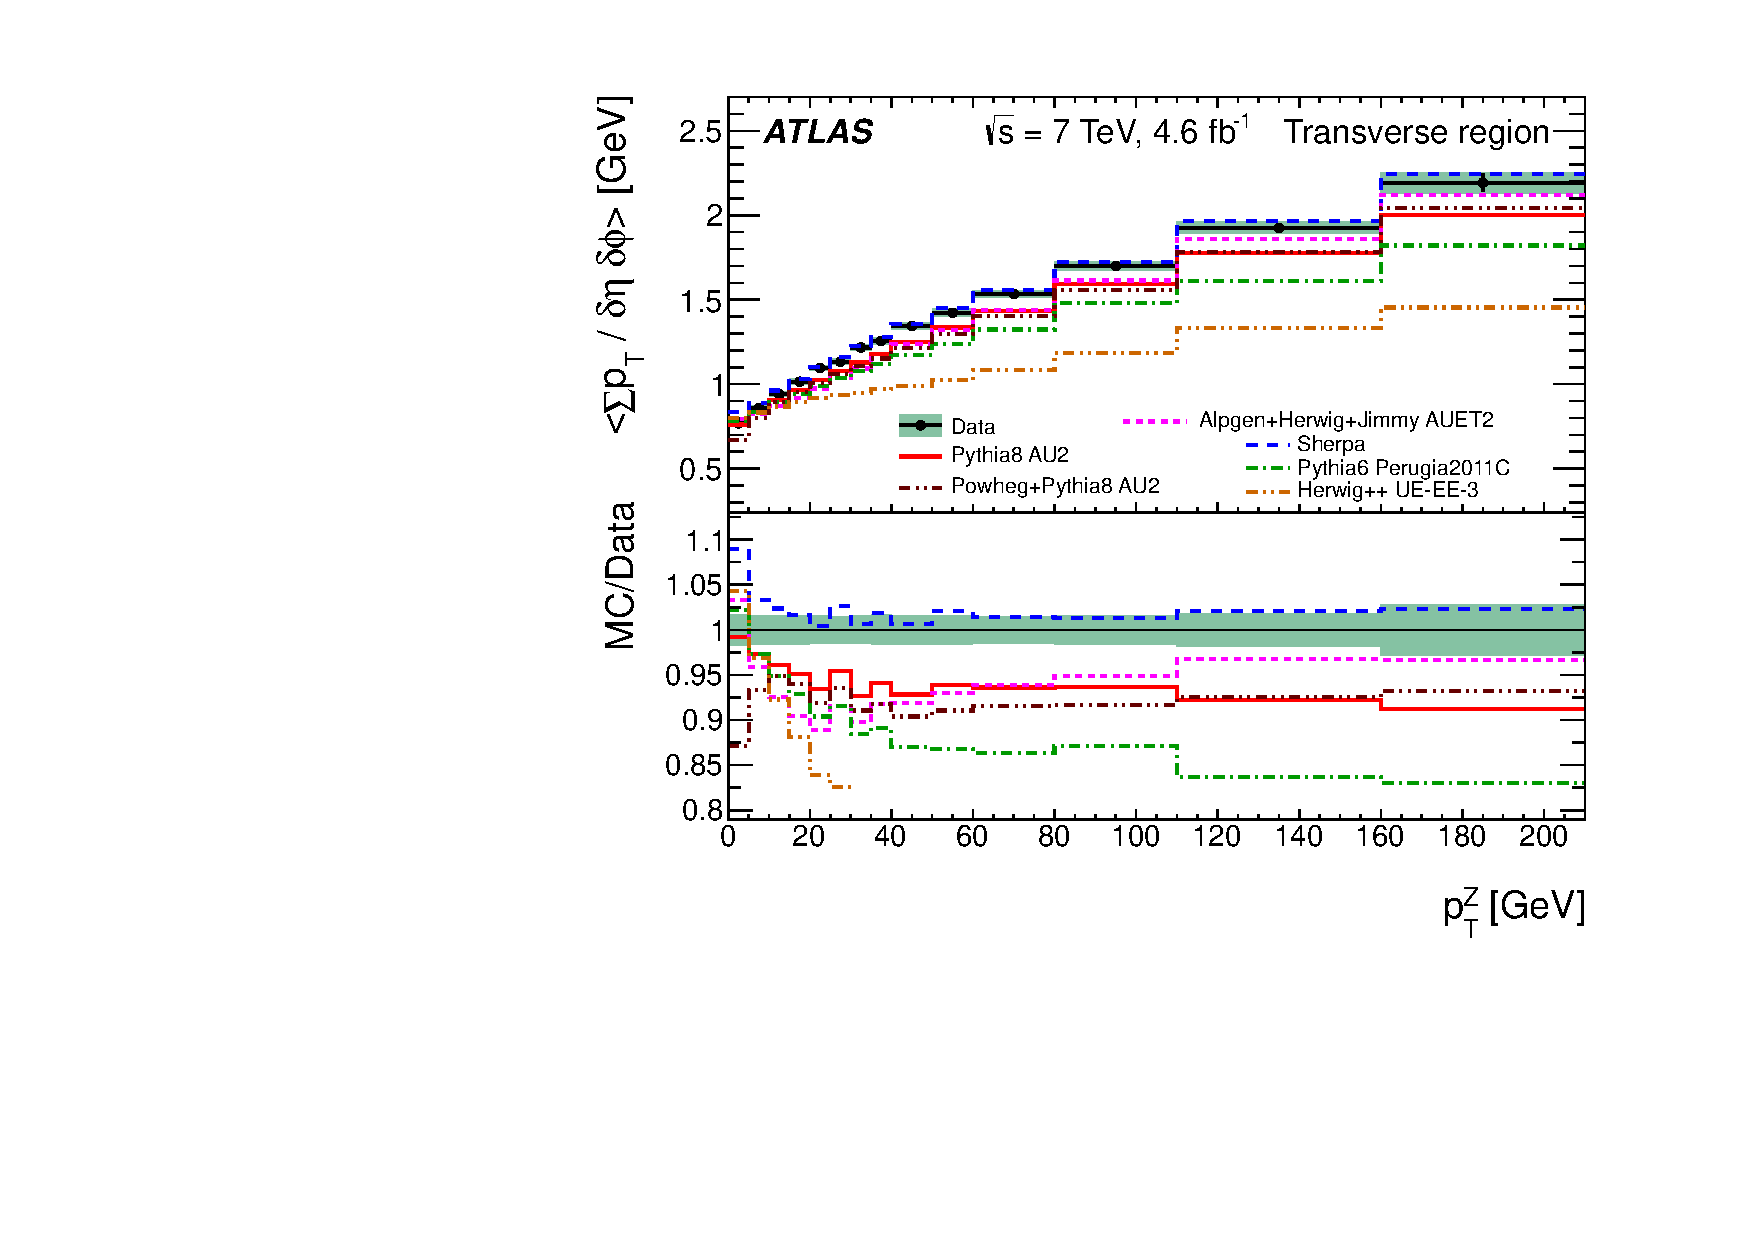
\includegraphics[width=0.48\textwidth]{figures/STDM-2011-42/fig_14b}
  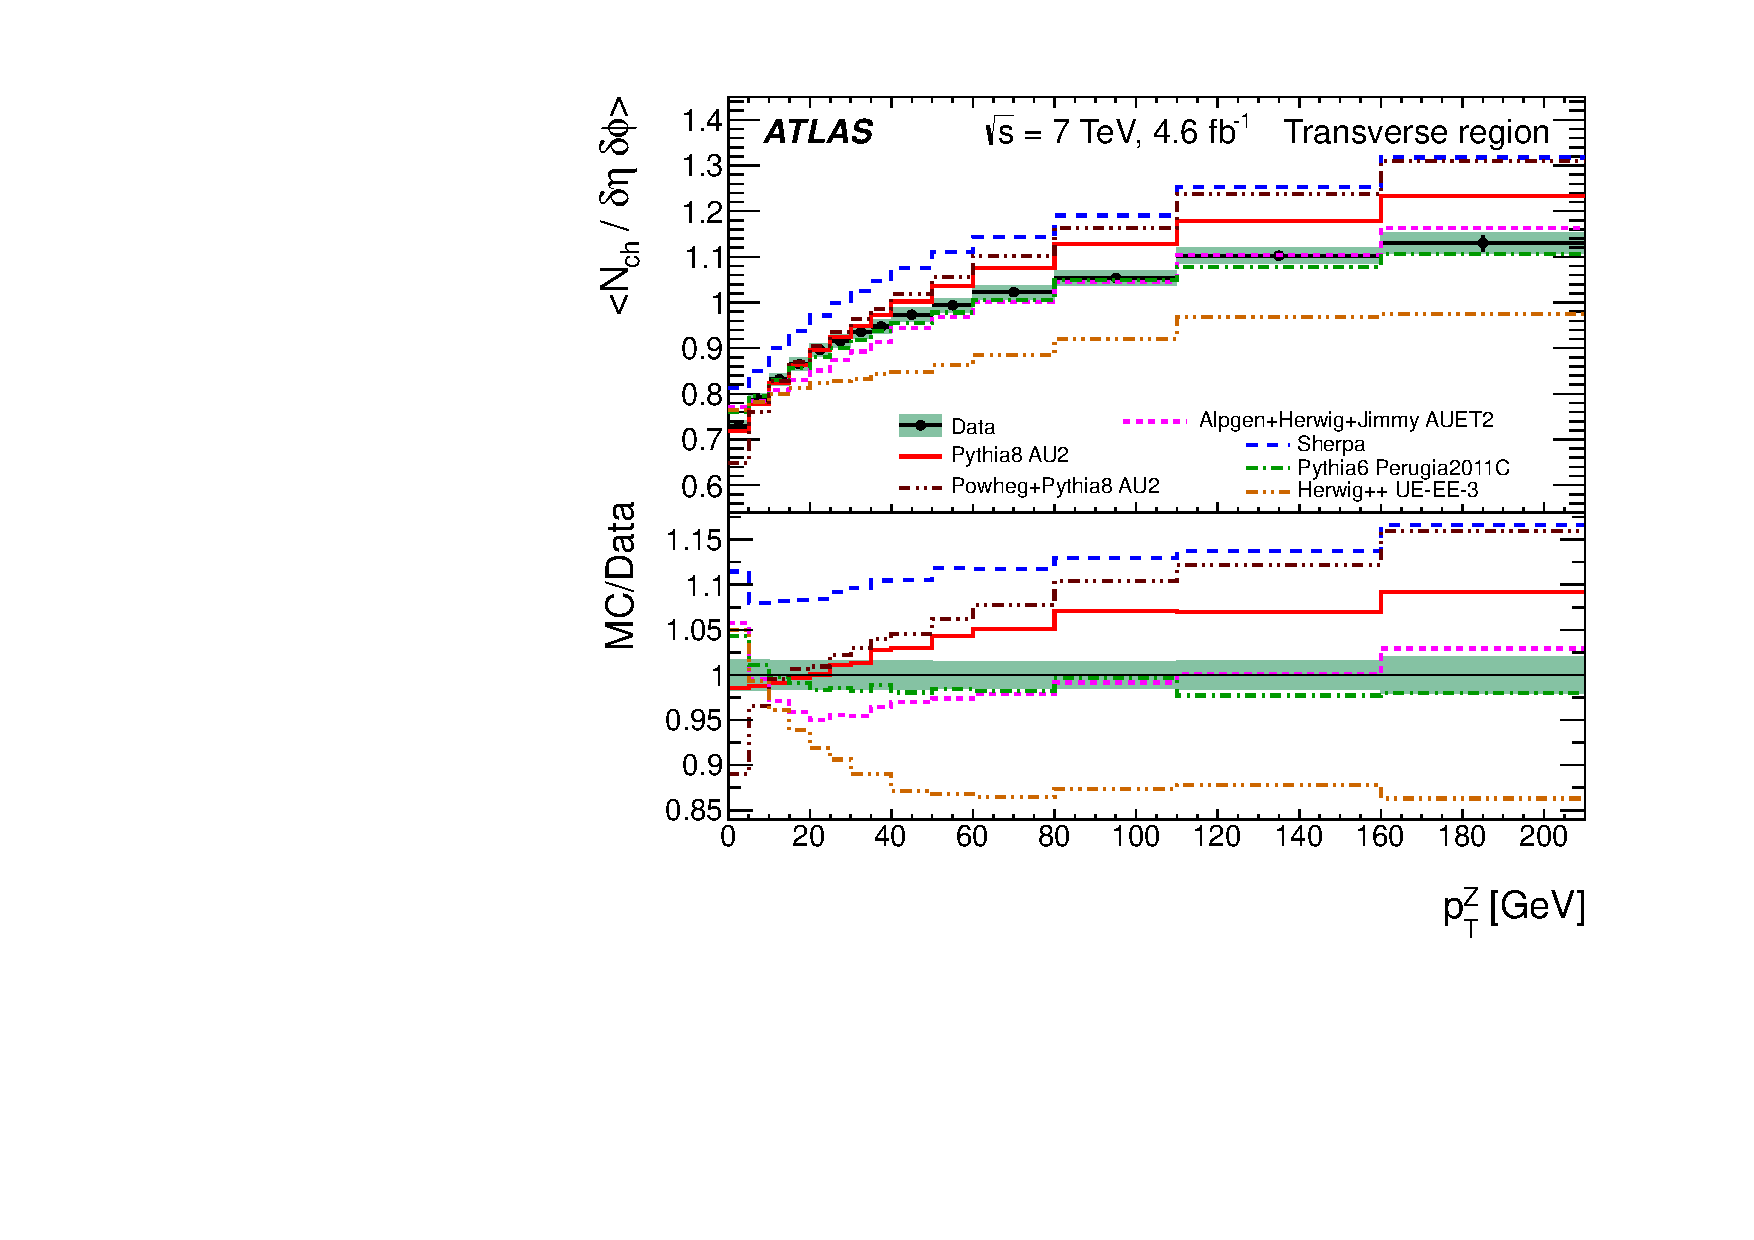
\includegraphics[width=0.48\textwidth]{figures/STDM-2011-42/fig_17b}
  \caption{Comparison of data and various predictions in $\Zll$ events of the charged particle scalar momentum density (left) and multiplicity density (right) as a function of $\pt^Z$ in 2011 data-taking~\cite{STDM-2011-42}. Mis-modeling is observed for all predictions.}
  \label{fig:backgrounds-zue}
\end{figure}

\begin{figure}[tp]
  \centering
  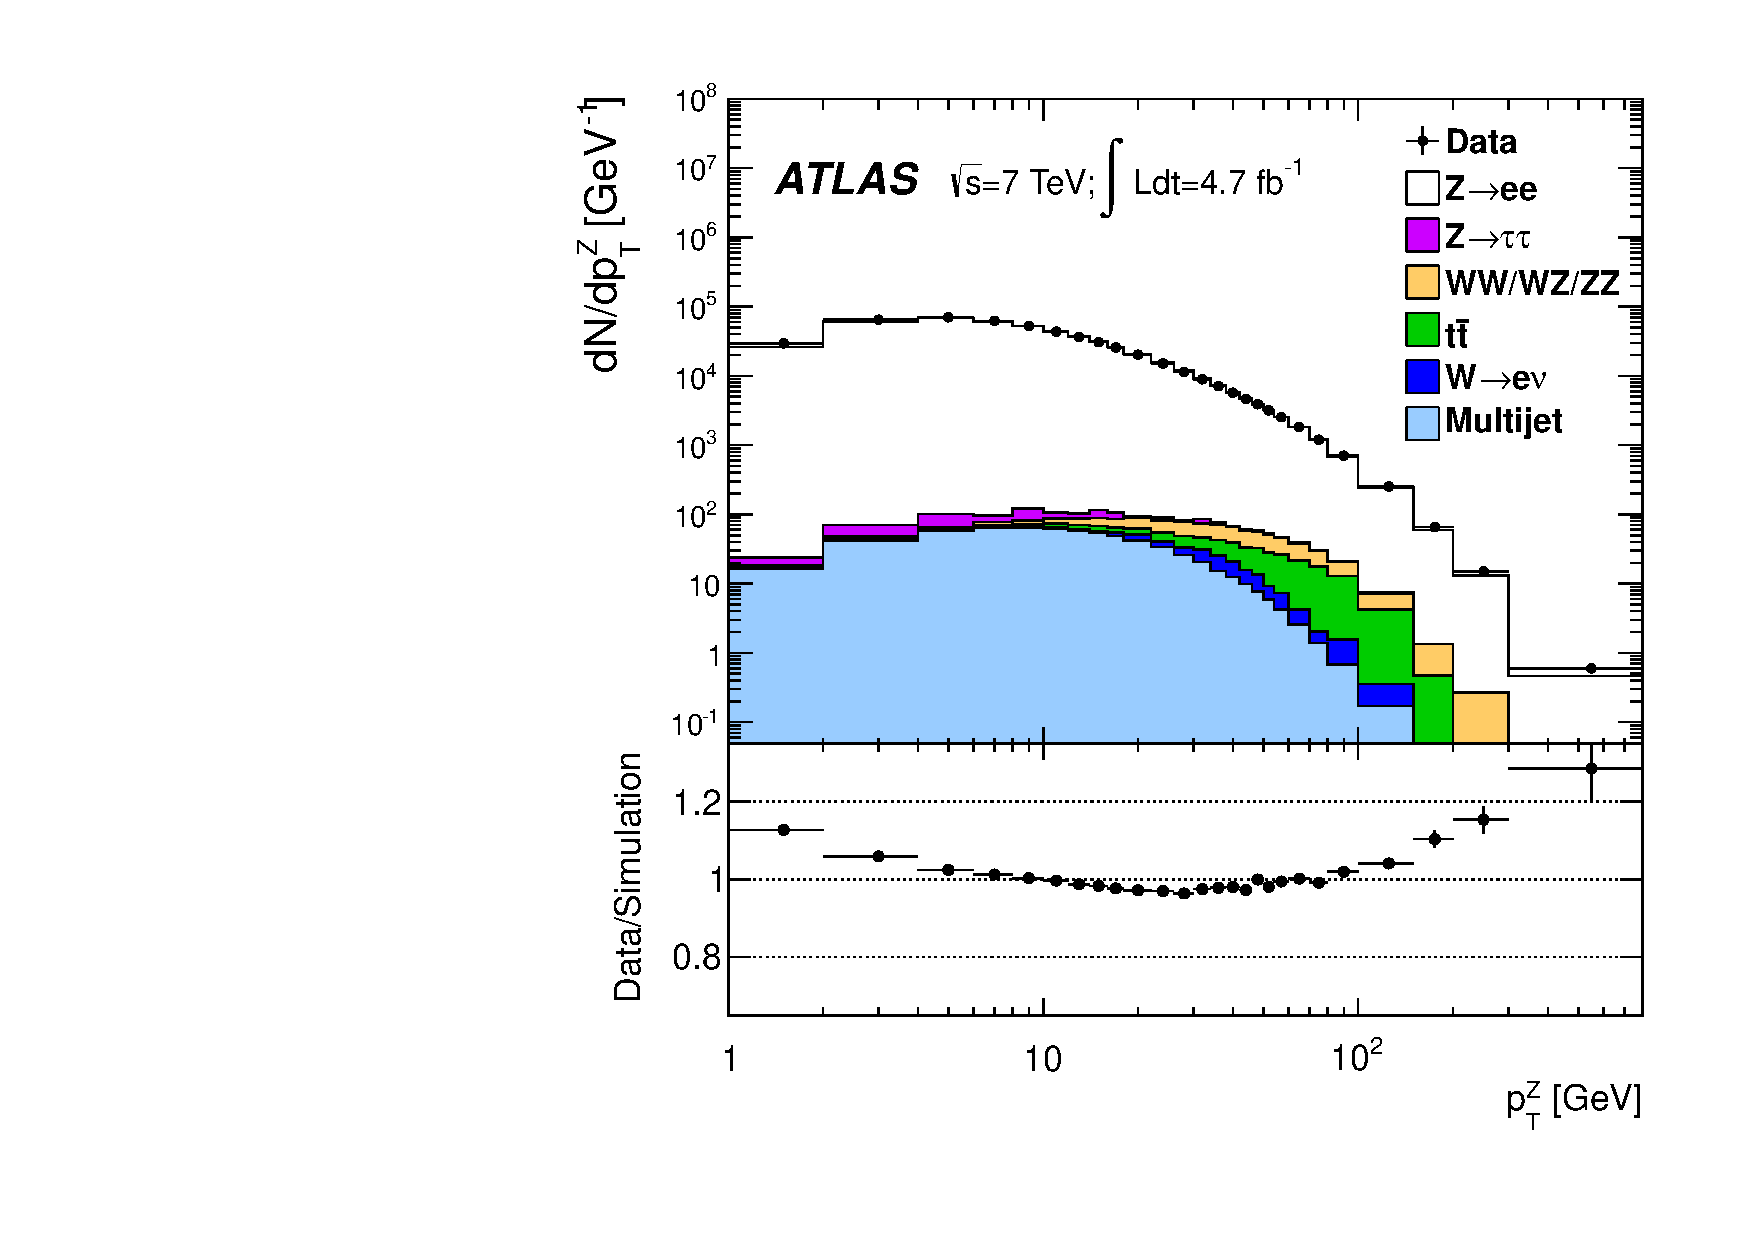
\includegraphics[width=0.48\textwidth]{figures/STDM-2012-23/fig_01a}
  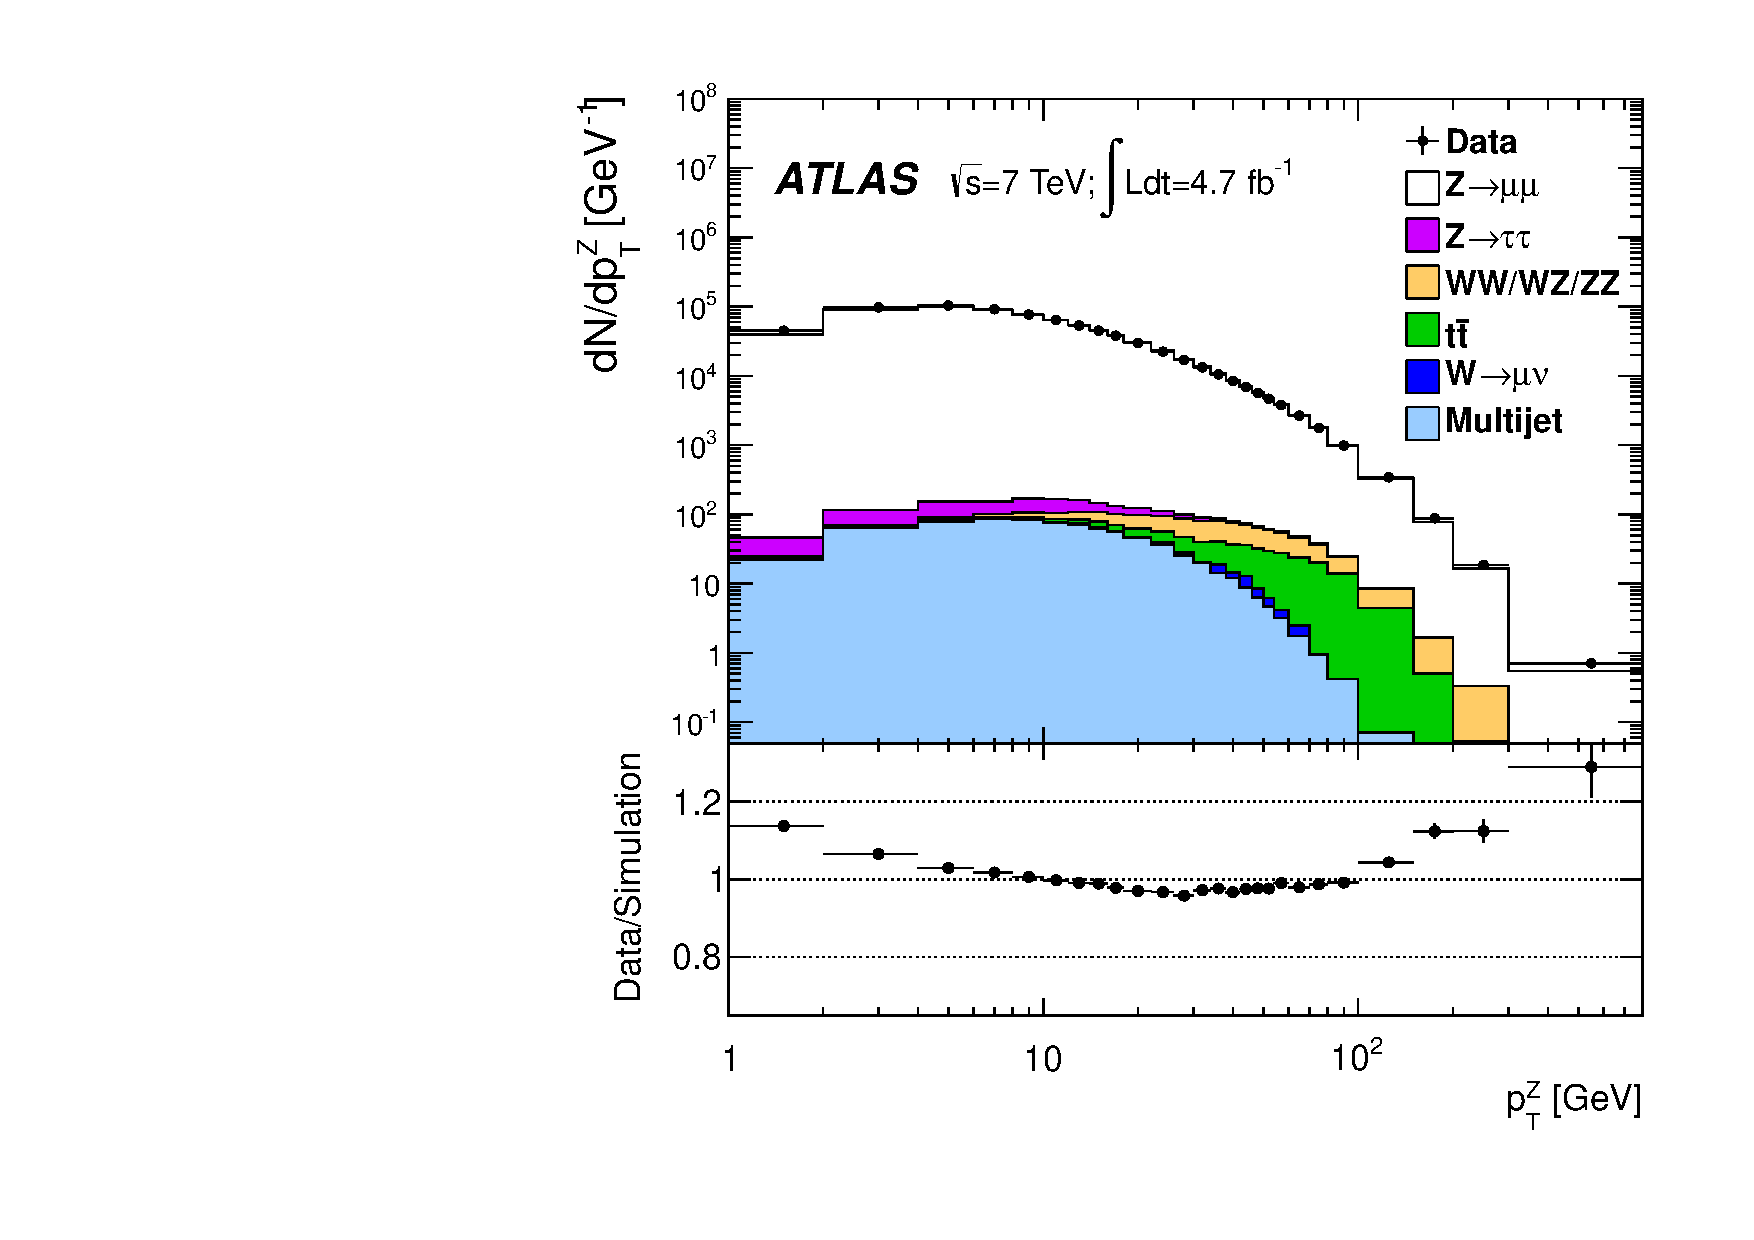
\includegraphics[width=0.48\textwidth]{figures/STDM-2012-23/fig_01b}
  \caption{Comparison of data and various predictions of $\pt^Z$ for $\Zee$ (left) and $\Zmm$ (right) in 2011 data-taking~\cite{STDM-2012-23}. Mis-modeling is observed.}
  \label{fig:backgrounds-zpt}
\end{figure}

\begin{figure}[tp]
  \centering
  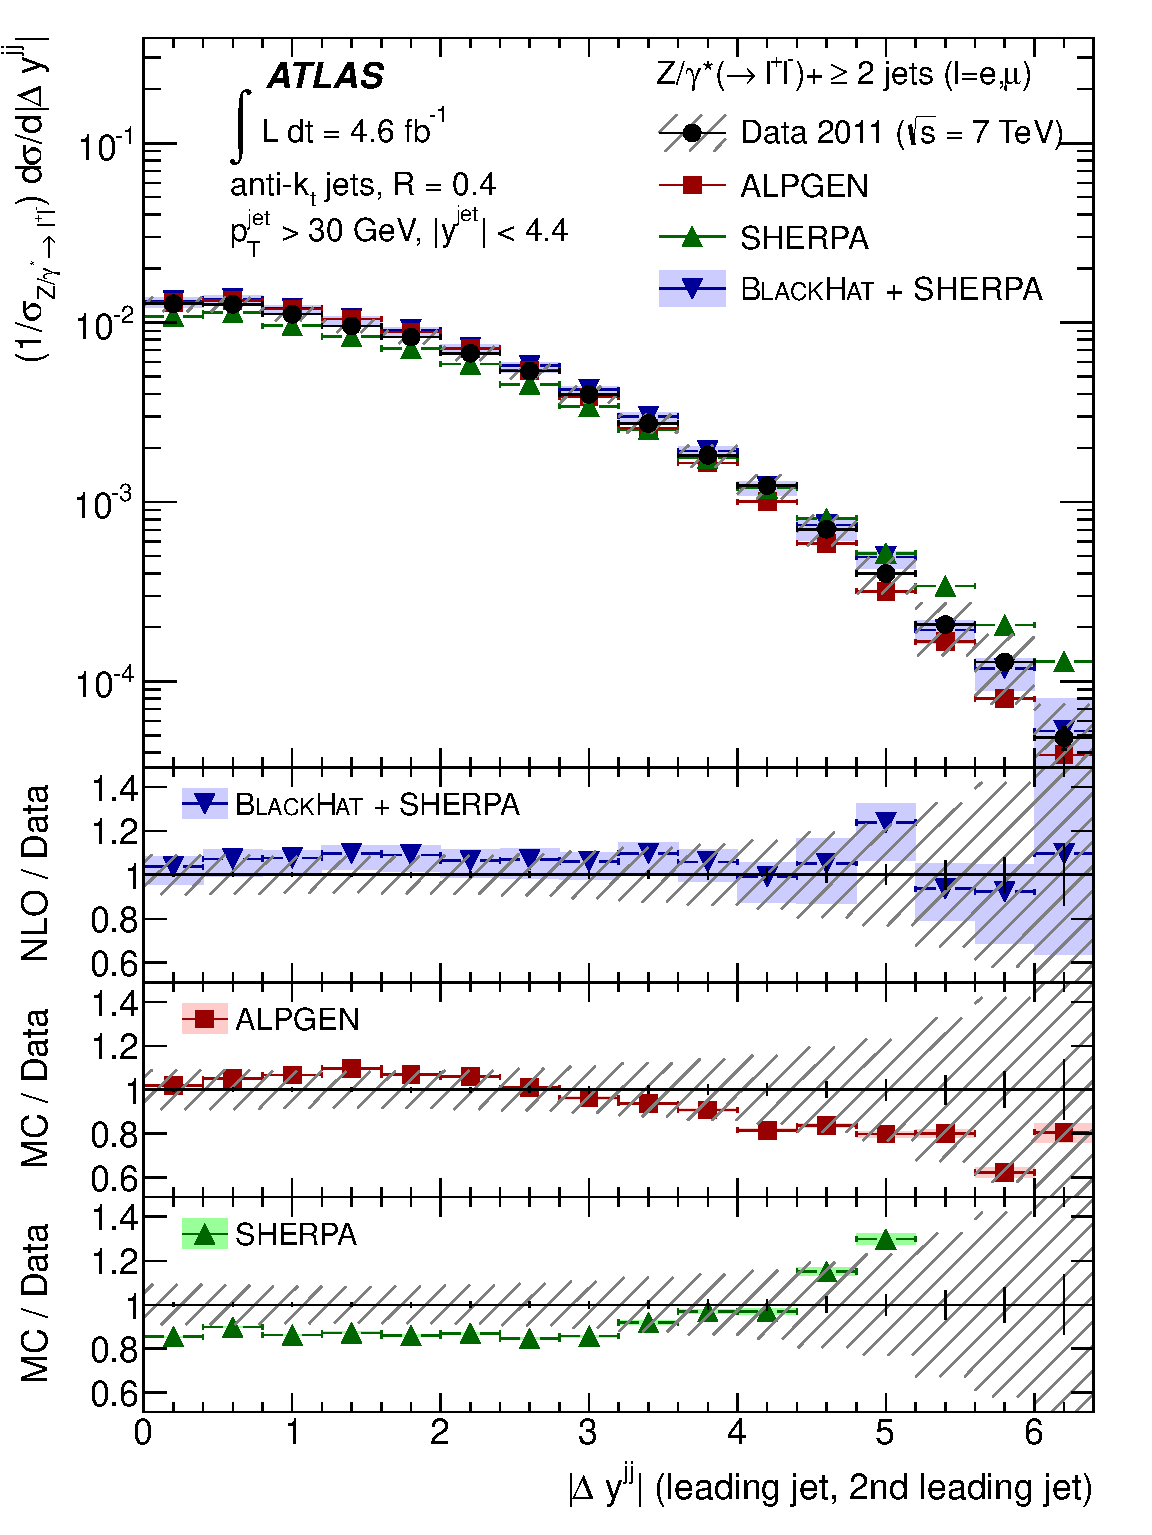
\includegraphics[width=0.48\textwidth]{figures/STDM-2012-04/fig_11a}
  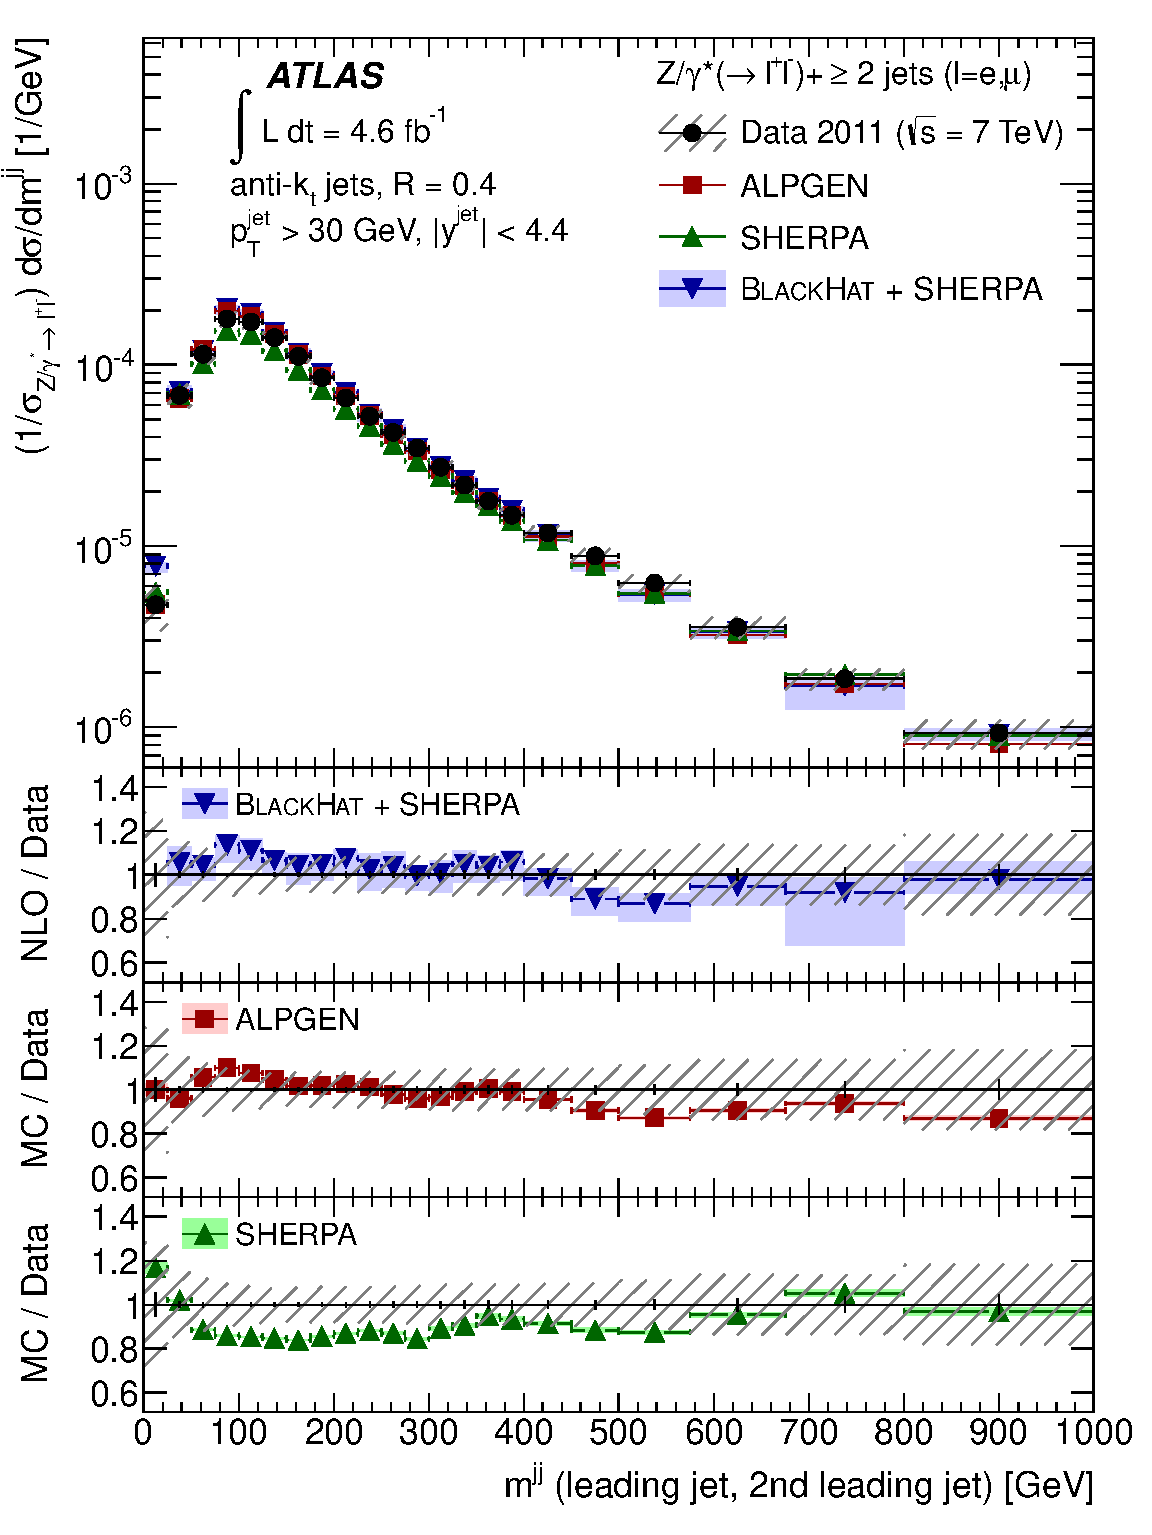
\includegraphics[width=0.48\textwidth]{figures/STDM-2012-04/fig_11b}
  \caption{Comparison of data and various predictions in $\Zll$ events of $\Delta y(jj)$ (left) and $\mjj$ (right) in 2011 data-taking~\cite{STDM-2012-04}. Mis-modeling is observed for all predictions.}
  \label{fig:backgrounds-zjj}
\end{figure}

These mis-modelings are worrisome for $\Htautau$ analyses because accurate modeling of these kinematics is relied on in the analysis. For example, mis-modeling in $\pt^Z$ is problematic because this variable defines the boosted category of the $\Htautau$ analysis. It is also strongly correlated with discriminating variables like $\Delta R(\tautau)$. Mis-modeling in dijet kinematics like $\mjj$ is of even greater concern because they are among the most powerful and high-profile discriminating variables in the VBF category.

Some versions of the ATLAS $\Htautau$ analysis use simulated $\Ztautau$ with corrections derived from $\Zll$ events in data~\cite{ATLAS-CONF-2012-160}. While helpful, these corrections are one-dimensional and cannot account for potential correlations in the mis-modeling. For these reasons, this approach is not used in the recent publication.

\subsection{Embedding}

A more data-driven approach to modeling $\Ztautau$ is used wherein $\Zmumu$ events are tagged in data and the muons are replaced with simulated tau lepton decays. This exploits lepton universality in $Z$ decays and has the great advantage of taking all $Z\!+\text{jets}$ features directly from data, such as $Z$ $\pt$, dijet kinematics, and soft hadronic activity. Only the tau lepton decays and the detector response of the decay products are taken from simulation. The former is measured with excellent precision at $B$-factories~\cite{2014.hfag}, and the latter is an ongoing area of study within ATLAS detector performance groups.

$\Zmumu$ events are selected in data by requiring an event fire the lowest unprescaled dimuon trigger and have at least two reconstructed muons with $\pt > 15$ GeV and $|\eta| <$ 2.5. All possible pairs of muons are then considered which satisfy $\pt^\text{lead} > $ 20 GeV, muon isolation requirements, have opposite charges, and have $m_{\mu\mu} > $ 40 GeV. The pair which has mass closest to the $Z$ mass is then chosen as the $Z$ decay products.

Tau lepton decays are then simulated with \texttt{TAUOLA} with the same four-momenta as the muons associated to the $Z$ decay and sent through the full ATLAS detector simulation, digitization, and reconstruction. The decays can be set to whatever final state desired (e.g., $\tautaueh$) within \texttt{TAUOLA}. 

The simulated $\tautau$ system is then merged with the data $\Zmumu$ event by removing tracks and calorimeter cells associated to the muons and inserting tracks and cells from the tau lepton decays. For subtracting the calorimeter cells, deposited cell energies are derived from a simulated $\Zmumu$ event with the same kinematics as the data $\Zmumu$ event. The hybrid event, with a simulated $\tautau$ system and a $Z\!+\text{jets}$ event from data, is then re-run through the ATLAS reconstruction, yielding the so-called \textit{embedded} $\Ztautau$ event. Event displays of this procedure is shown in \cref{fig:backgrounds-embedding-eventdisplay}.

\begin{figure}[tp]
  \centering
  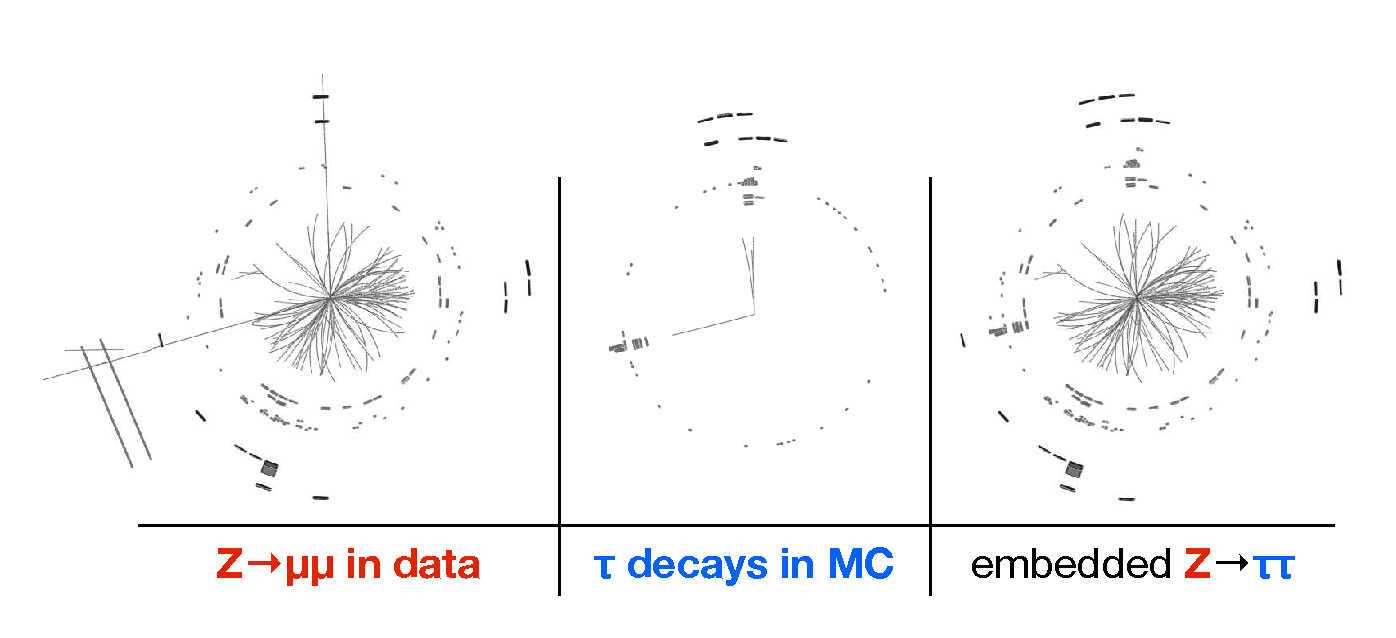
\includegraphics[width=0.95\textwidth]{figures/backgrounds/embedding_eventdisplay}
  \caption{Event displays of the three types of events considered in the embedding procedure: a $\Zmumu$ event in data (left), a $\tautauhh$ event in simulation (center), and a hybrid embedding event (right)~\cite{ATL-COM-PHYS-2012-1201}.}
  \label{fig:backgrounds-embedding-eventdisplay}
\end{figure}

\subsection{Validation}

Various steps of the embedding procedure are validated with creative choices of output and input datasets of the embedding algorithms. For example, to test the subtraction of data muons, the embedding procedure is run on data $\Zmumu$ events merged with simulated $\Zmumu$ decays, and the output is compared with the original data $\Zmumu$ events. For a global test of the fidelity of the method, the embedding procedure is run on simulated $\Zmumu$ events merged with simulated $\Ztautau$ decays, and the output is compared with simulated $\Ztautau$ events. The results are shown in \cref{fig:backgrounds-embedding-validation}, and no significant biases are observed.

\begin{figure}[tp]
  \centering
  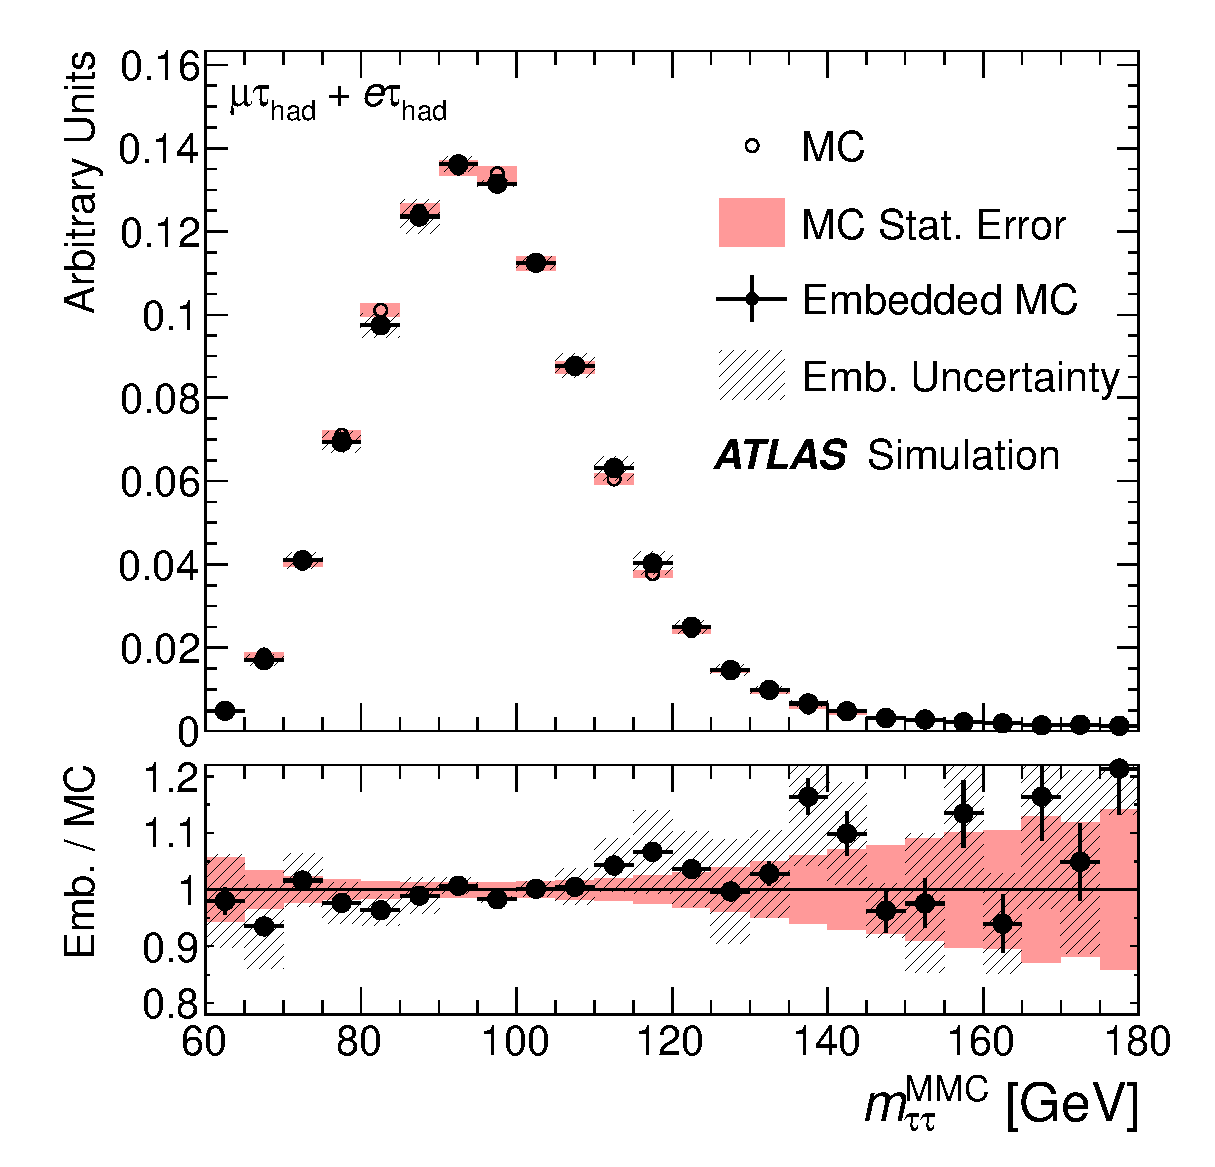
\includegraphics[width=0.48\textwidth]{figures/HIGG-2013-32/fig_03b}
  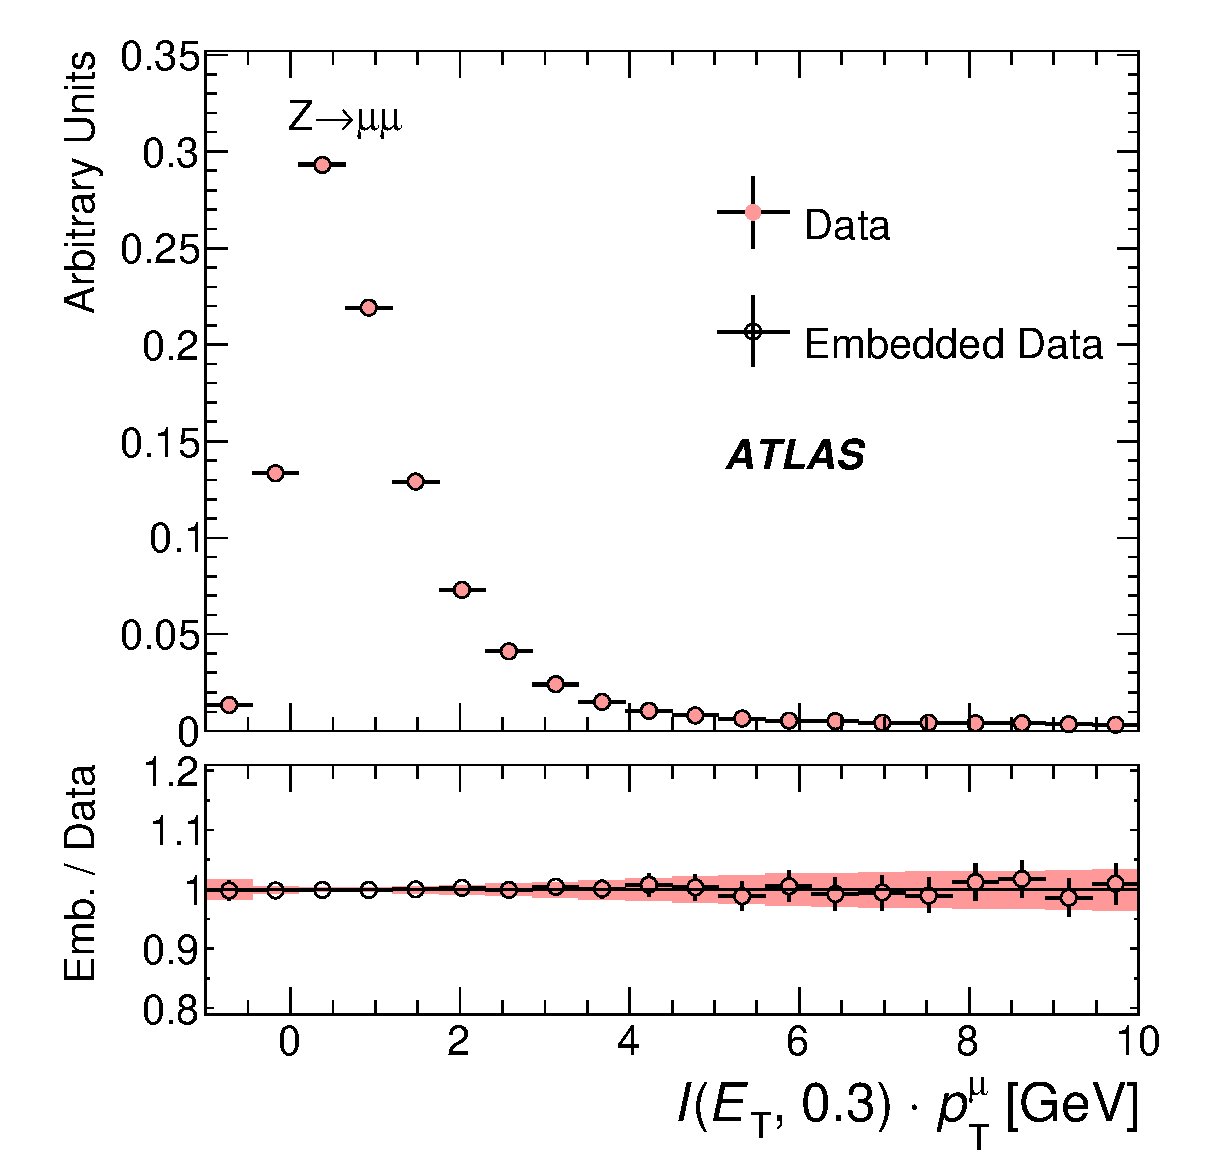
\includegraphics[width=0.48\textwidth]{figures/HIGG-2013-32/fig_03a}
  \caption{Validation of the embedding technique for simulated tau lepton decays in simulated $\Zmm$ events (left) and simulated muons in data $\Zmm$ events (right)~\cite{HIGG-2013-32}. Good agreement is observed in both.}
  \label{fig:backgrounds-embedding-validation}
\end{figure}

\clearpage

\subsection{Uncertainties}

Since all $Z$ kinematics are taken directly from data, no uncertainties regarding to $Z$ or jet kinematics are considered. However, uncertainties regarding the response of simulating tau decay products and the embedding procedure itself are considered. The uncertainty on the detector response is implemented via the typical collection of uncertainties pertaining to the measured identification efficiency and energy calibration of simulated leptons and $\tauh$ at ATLAS.

Two uncertainties regarding the embedding procedure are considered. First, the isolation criteria on the data muons are either relaxed or tightened to test the dependence of the prediction on the $\Zmumu$ selection criteria. Second, the amount of cell energy subtracted when removing the data muons is varied by 20\%, which is commensurate with the observed differences in the isolation energy between simulated $\Zmumu$ events merged with simulated $\Ztautau$ decays and simulated $\Ztautau$ events.

The pre-fit impact of these uncertainties on the $\Ztautau$ prediction is shown in each bin of the VBF discriminator in \cref{fig:backgrounds-uncertainties-Ztautau}. The largest uncertainty at high VBF BDT score is the nearly 30\% statistical uncertainty on the prediction, which is an inevitable limitation of the embedding procedure since it relies on the finite number of $\Zmumu$ events in data. The largest systematic uncertainties are component of the $\tauh$ energy scale uncertainty, which are each 10-15\%. These propagate directly to shifts of the $\mMMC$.

\begin{figure}[tp]
  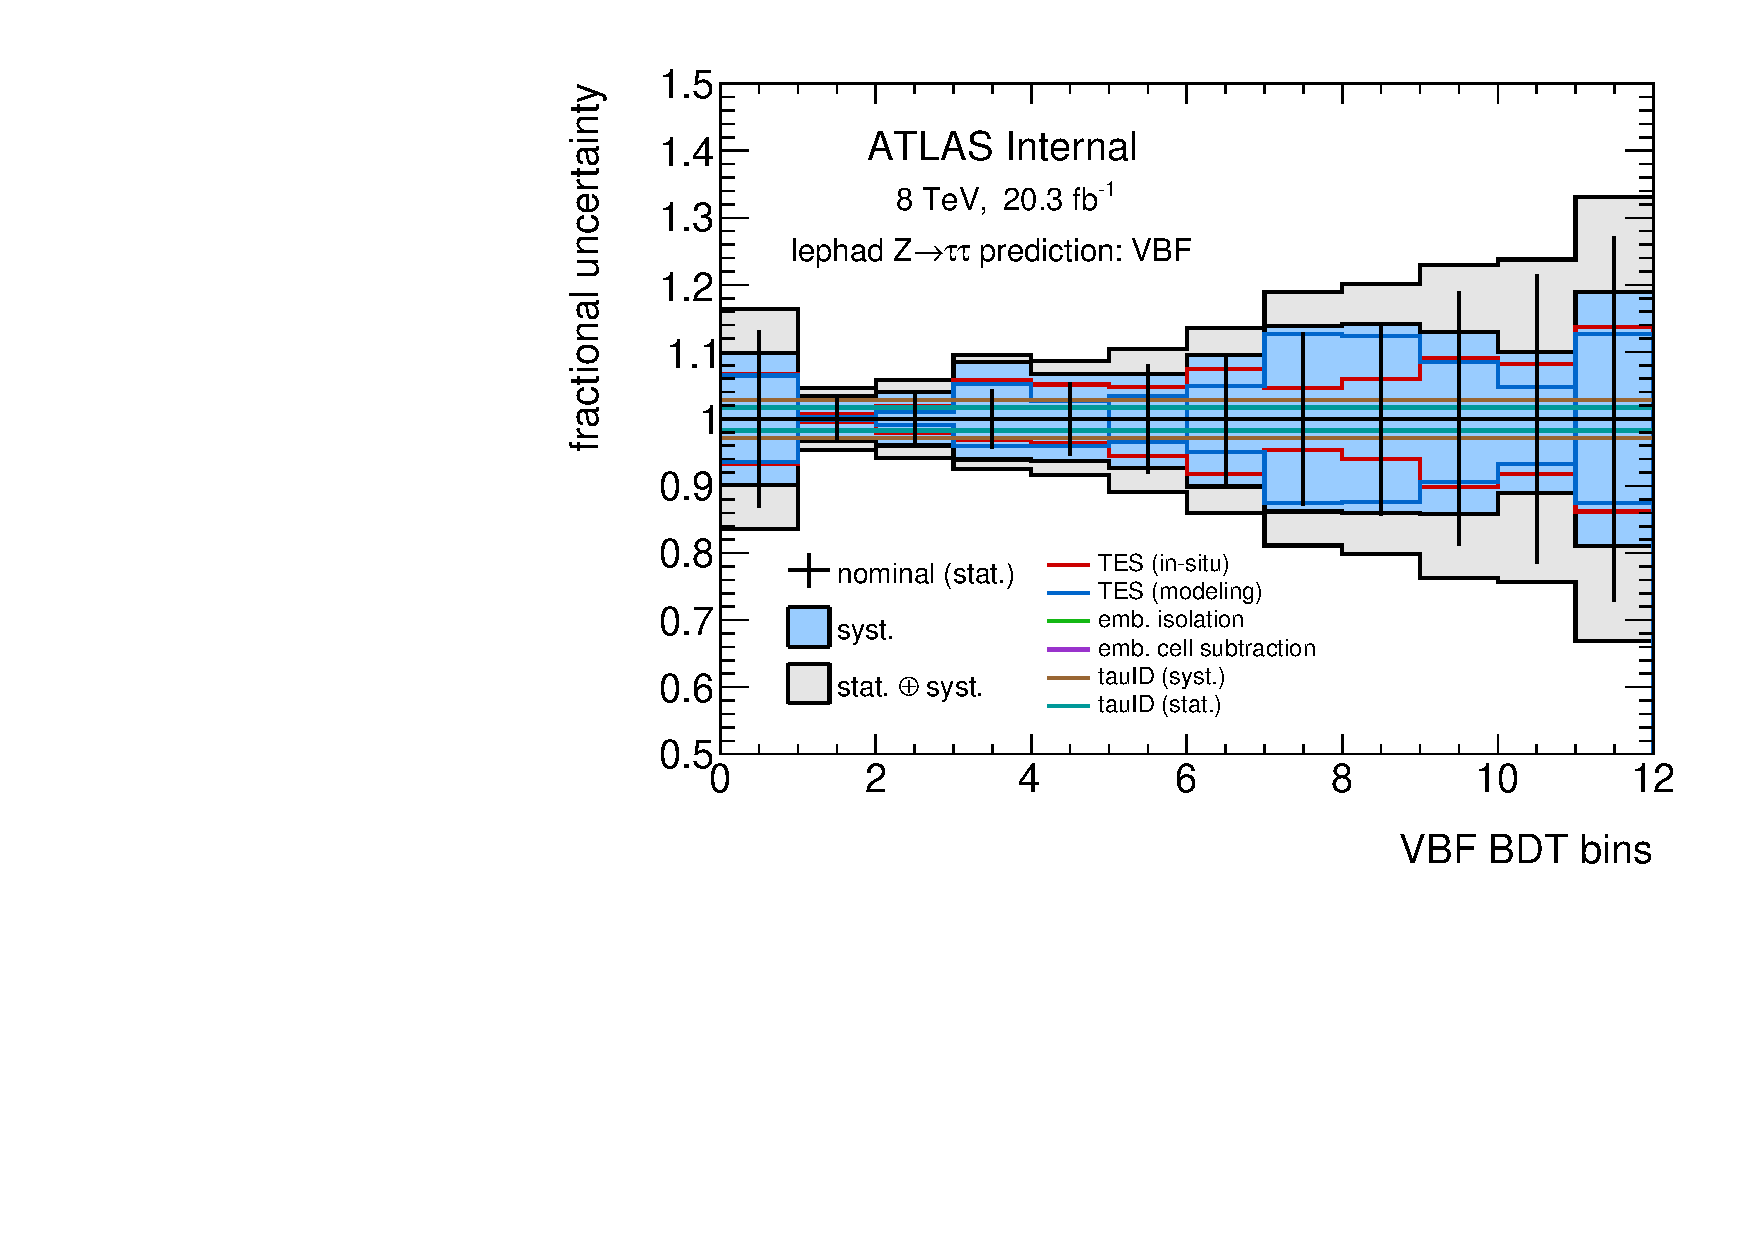
\includegraphics[width=0.90\textwidth]{figures/uncertainties/uncertainties_lephad_paper14_8TeV_Ztautau_VBF}
  \caption{The pre-fit fractional uncertainty on the embedded $\Ztautaulh$ prediction in each bin of the VBF category for uncertainties pertaining to the embedding procedure and $\tauh$ performance.}
  \label{fig:backgrounds-uncertainties-Ztautau}
\end{figure}

\clearpage
\section{$\fakes$ mis-identification}
\label{sec:backgrounds-misid}

The largest background in the VBF $\Htautaulh$ analysis is from events where a jet is mis-identified as a $\tauh$, $\fakes$. The use of data-driven approaches to the prediction is therefore crucial. Unlike the $\Ztautau$ background, many regions of data exist which are rich in $\fakes$, and these regions can be exploited. The largest sources of $\fakes$ are $\Wjets$, QCD, top, and $\Zjets$ events.

\subsection{Mis-modeling of $\fakes$ processes in simulation}

Like the $\Ztautau$ background, simulation is a simple but deficient means of predicting the $\fakes$ background. ATLAS observes mis-modeling in descriptions of jet shapes like the track width and track multiplicity~\cite{PERF-2013-02}, as shown in \cref{fig:backgrounds-trackwidth}, which $\tauh$ jet discriminators rely heavily on. This is especially problematic for $\tauh$ because the identification algorithms emphasize tails of distributions like track width, not the bulk, hence detailed corrections to the simulation can be statistically limited.

\begin{figure}[tp]
  \centering
  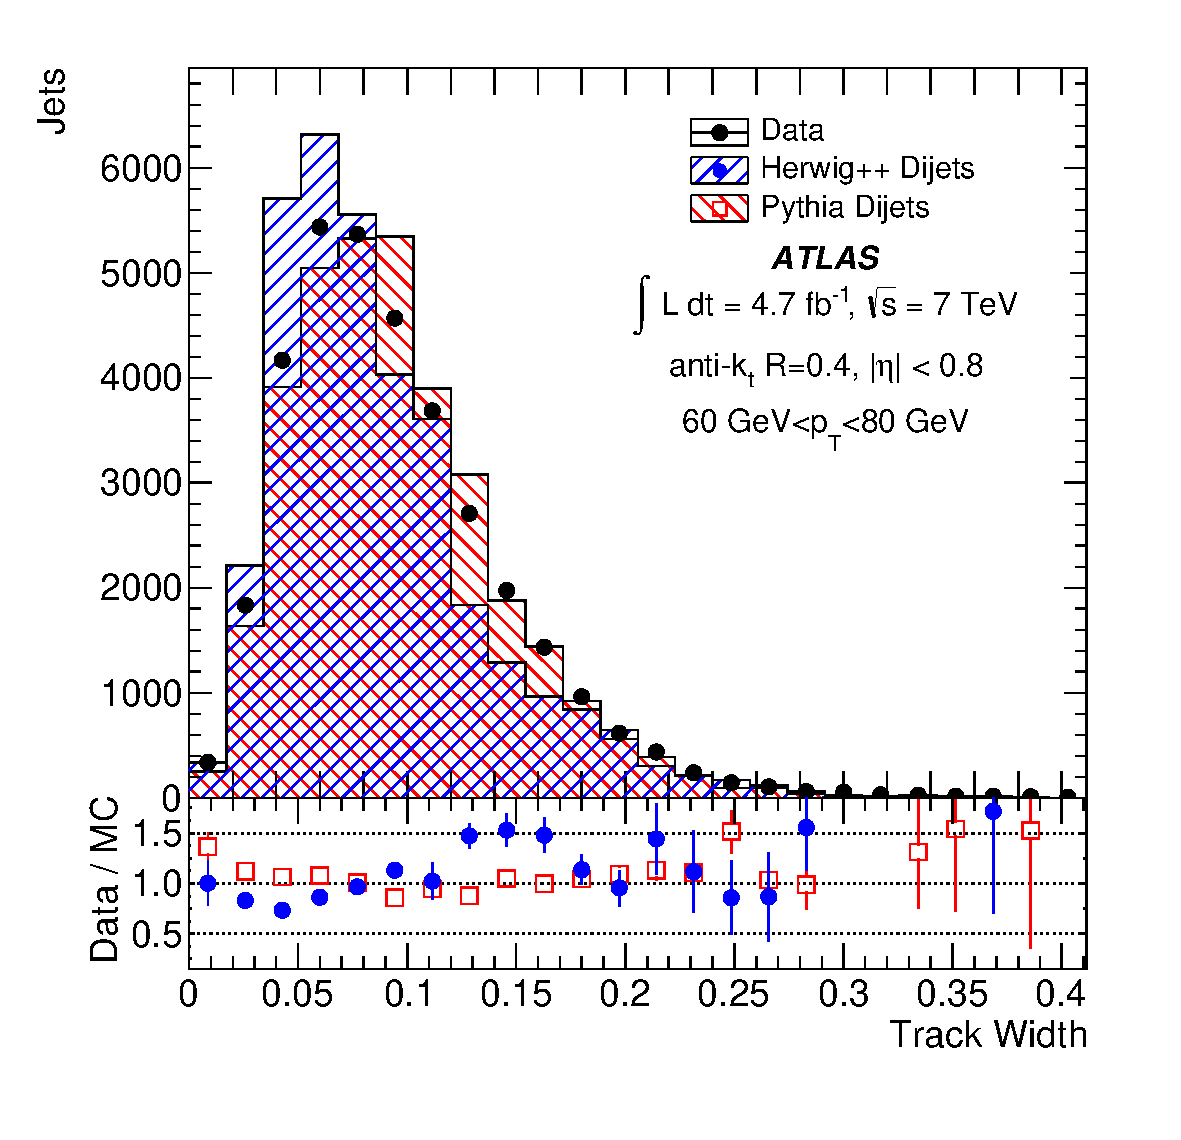
\includegraphics[width=0.45\textwidth]{figures/PERF-2013-02/figaux_01c}
  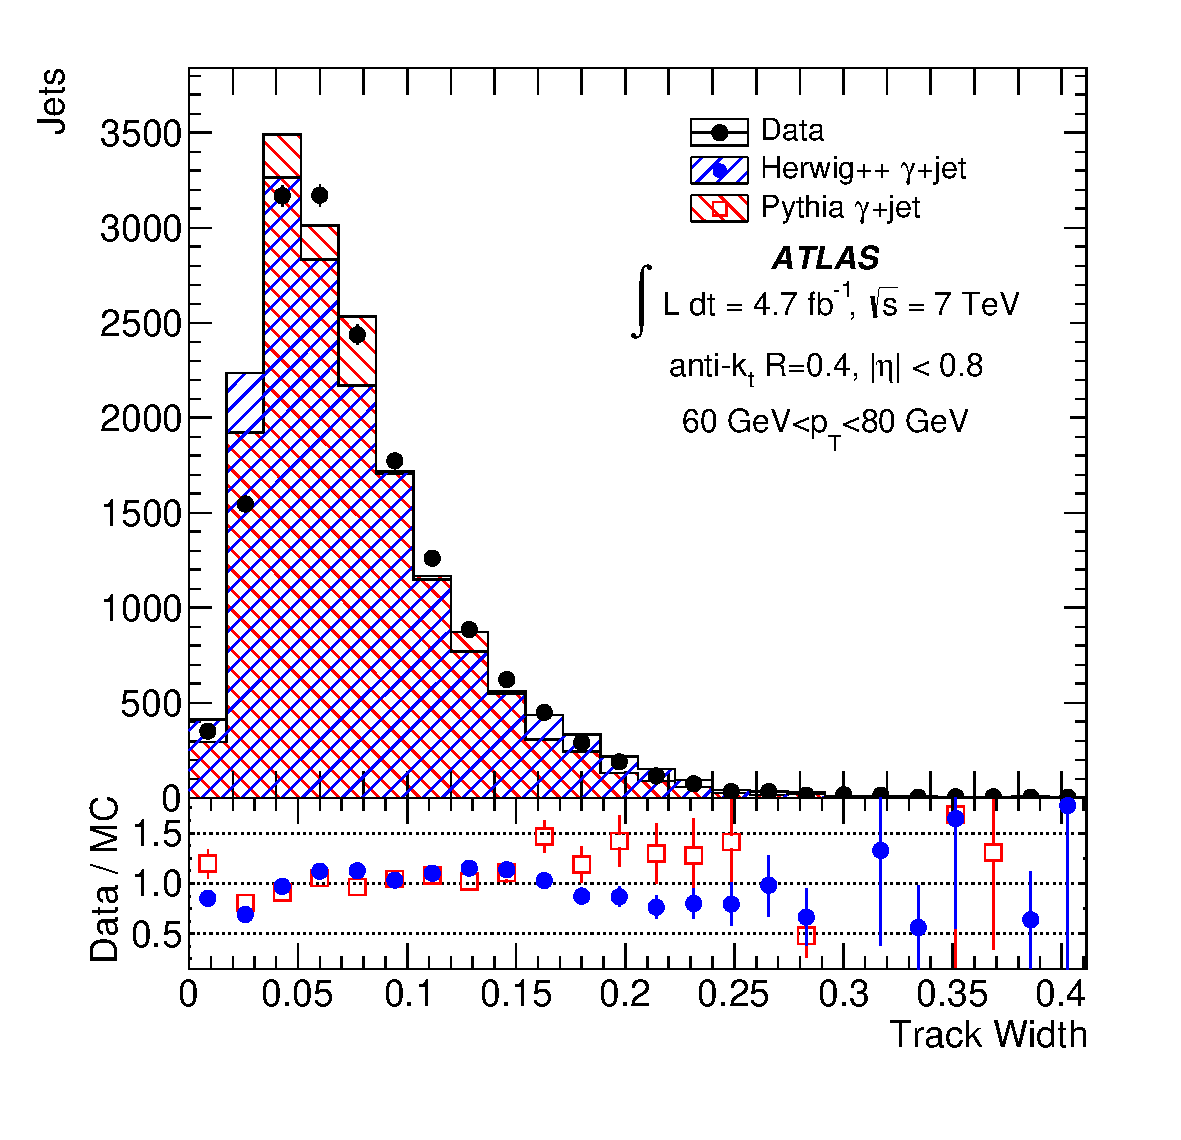
\includegraphics[width=0.45\textwidth]{figures/PERF-2013-02/figaux_02c}
  \caption{Comparison of data and various predictions of jet track width in dijet (left) and $\gamma\!+\!\text{jet}$ (right) events~\cite{PERF-2013-02}. Mis-modeling is observed for all predictions.}
  \label{fig:backgrounds-trackwidth}
\end{figure}

Additionally, the event kinematics of $\Wjets$ and $\Zjets$ events have known mis-modeling in simulation. The mis-modeling of $\Zjets$ events is discussed in \cref{sec:backgrounds-zjets}, and ATLAS observes comparable mis-modeling in dijet kinematics of $\Wjets$ events, as shown in \cref{fig:backgrounds-wjets}. The mis-modeling of variables like $\Delta y(jj)$ and $\mjj$ is of concern since the VBF discriminators depend heavily on these kinematics.

\clearpage
\begin{figure}[tp]
  \centering
  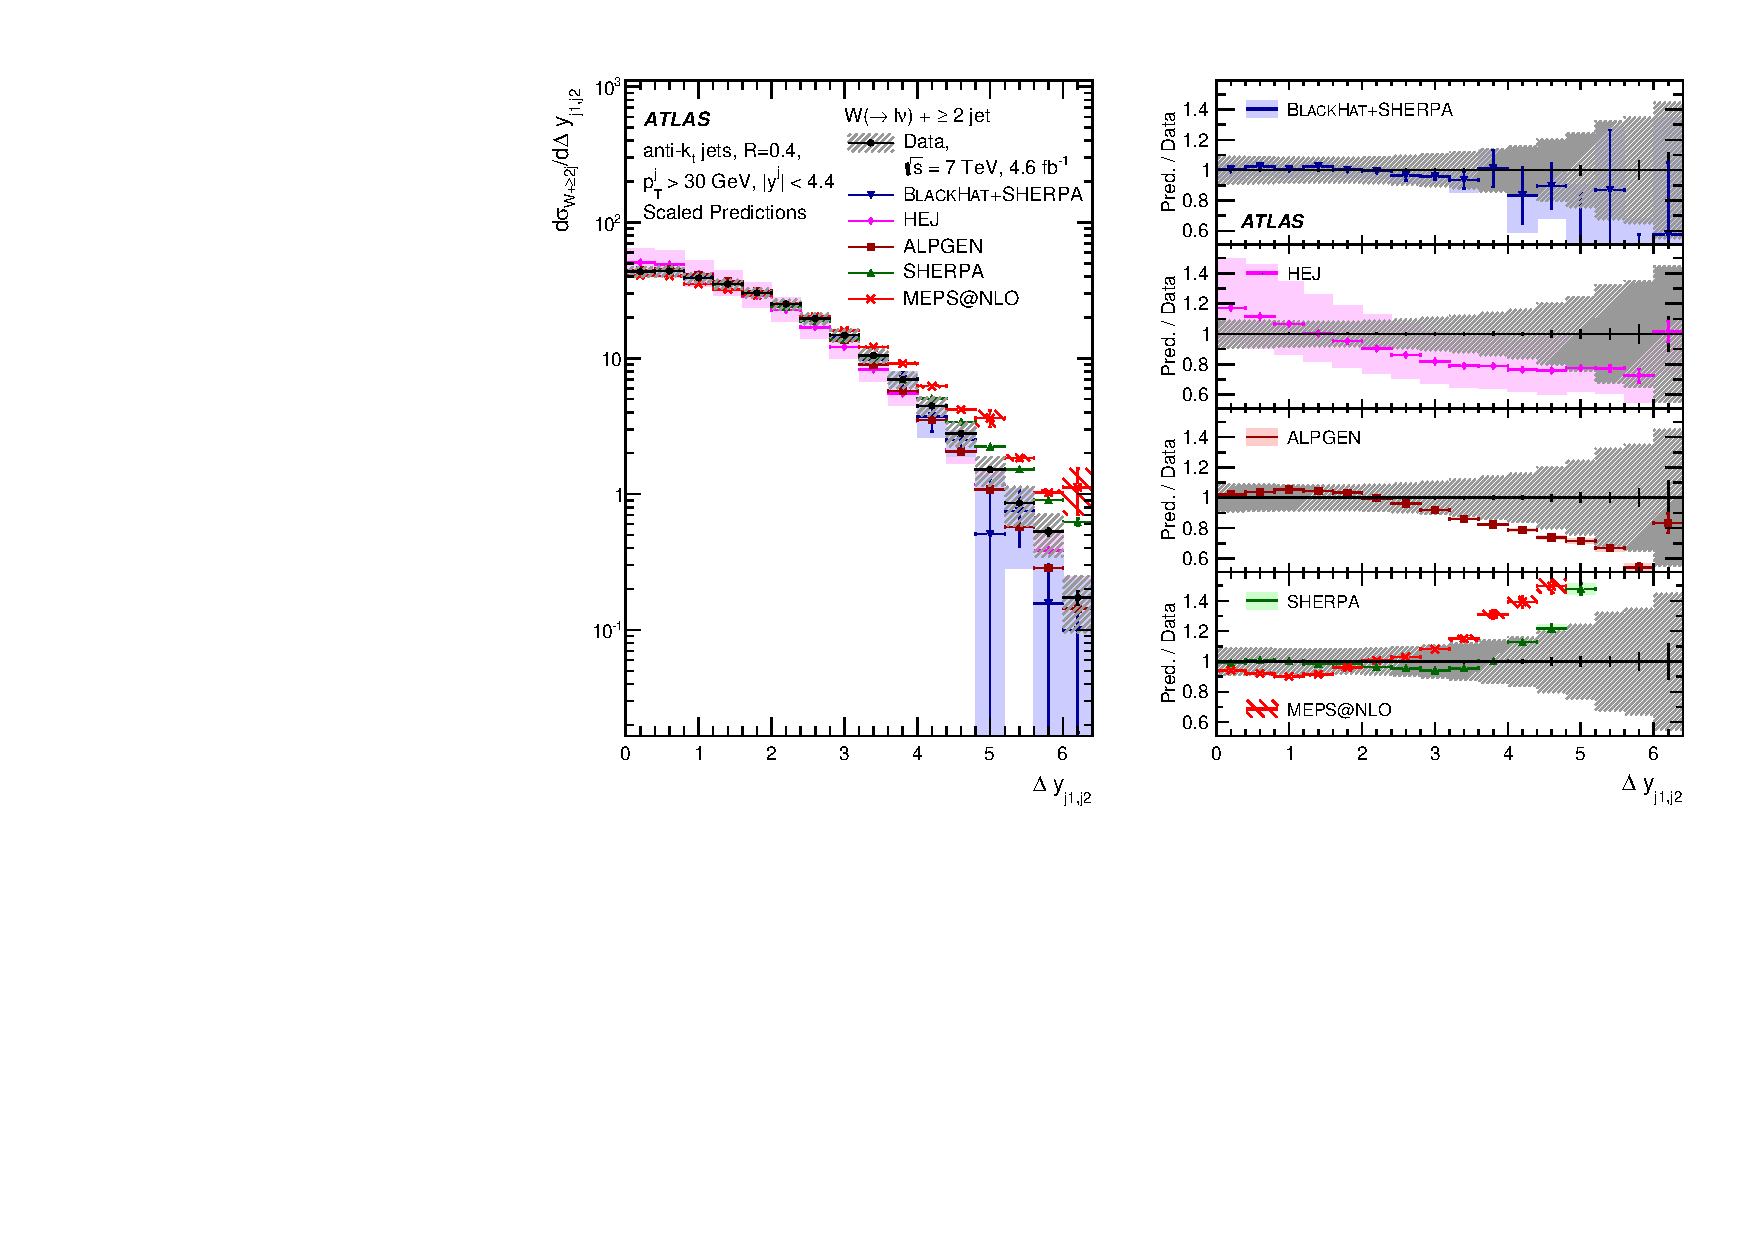
\includegraphics[width=0.90\textwidth]{figures/STDM-2012-24/fig_26a}
  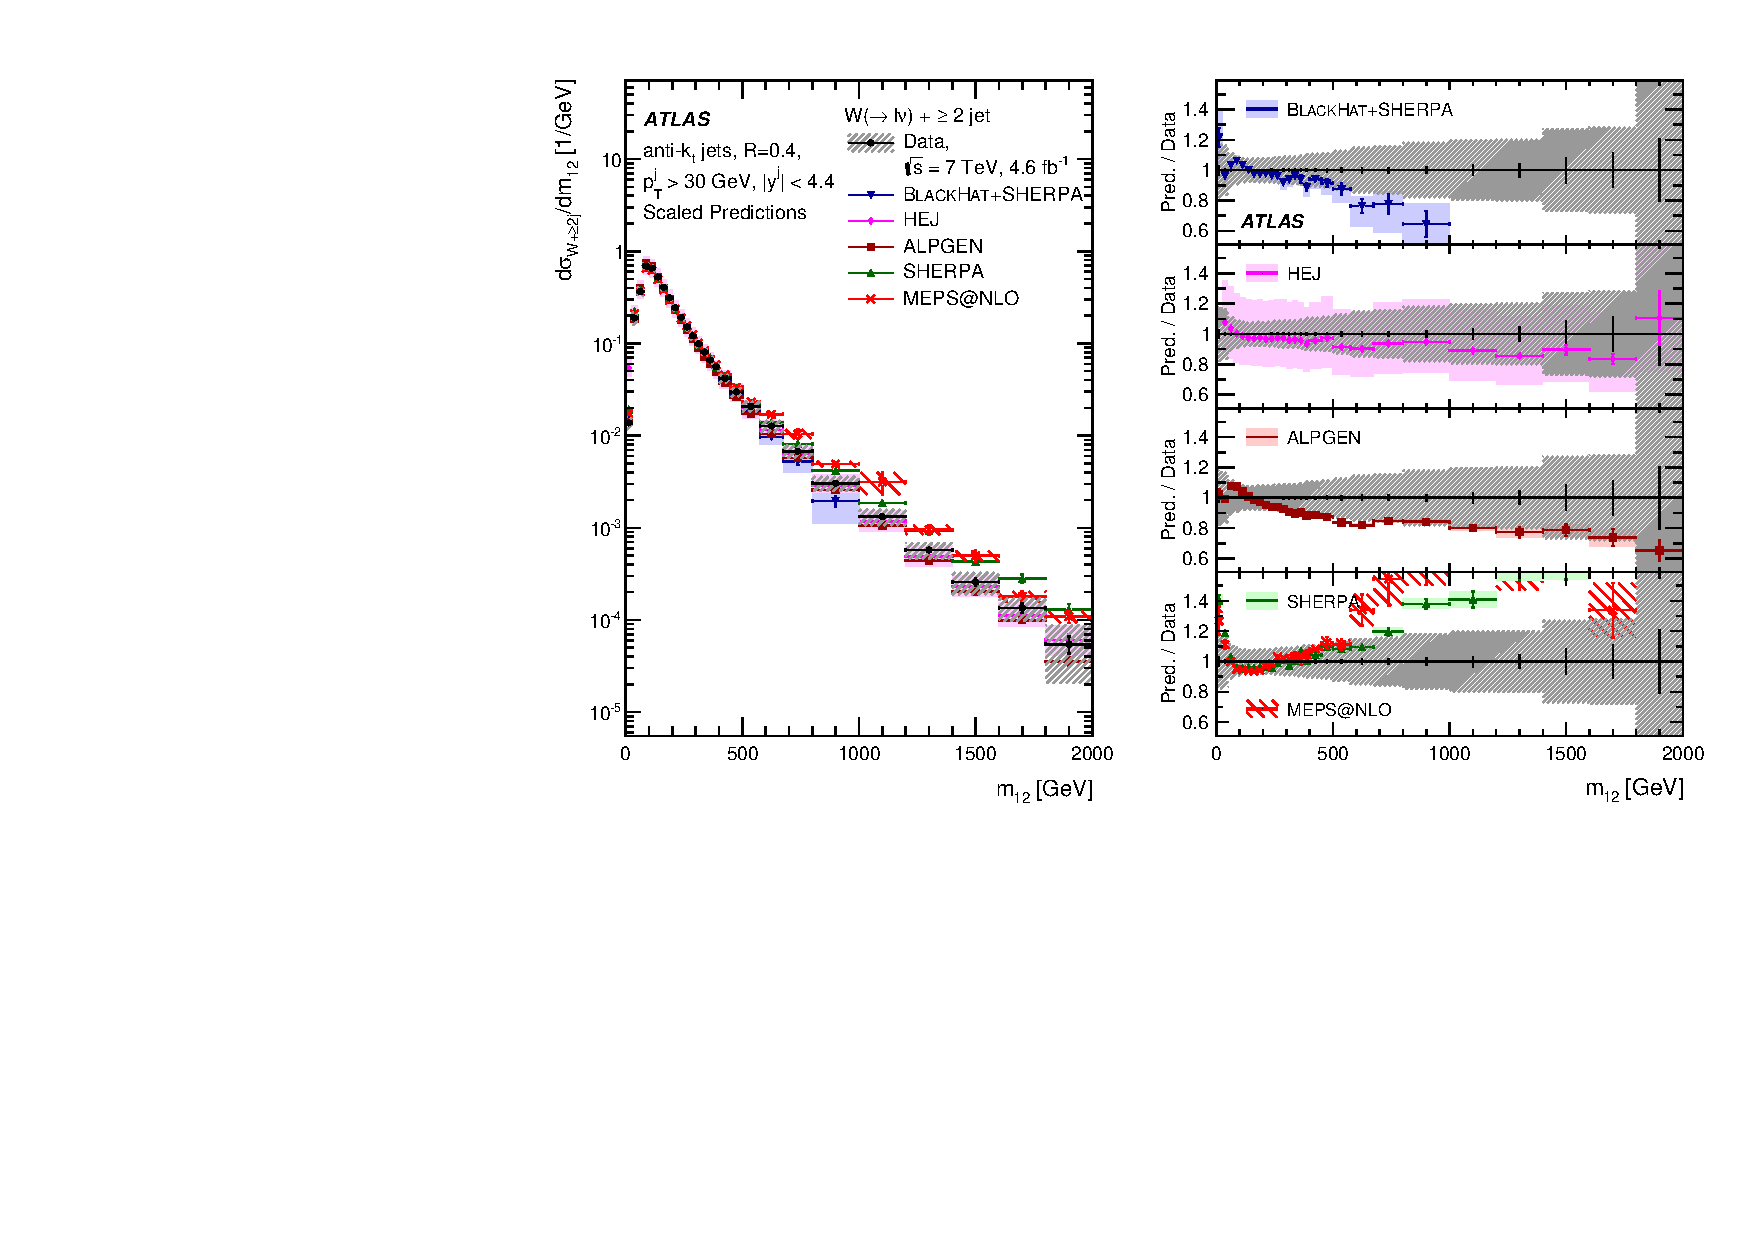
\includegraphics[width=0.90\textwidth]{figures/STDM-2012-24/fig_28a}
  \caption{Comparison of data and various predictions in $\Wjets$ events of $\Delta y(jj)$ (top) and $\mjj$ (bottom) in 2011 data-taking~\cite{STDM-2012-24}. Mis-modeling is observed for all predictions.}
  \label{fig:backgrounds-wjets}
\end{figure}
\clearpage

Some versions of the ATLAS $\Htautau$ analysis use simulated $\Wjets$, $\Zjets$, and top events with corrections derived from data, in conjunction to same-sign data events, to model $\fakes$~\cite{HIGG-2012-07,ATLAS-CONF-2012-160}. While helpful, these corrections are one-dimensional and cannot account for potential correlations in the mis-modeling, and the same-sign data sample has large statistical uncertainties. For these reasons, this approach is not used in the recent publication.

\subsection{Fakefactor method}

\subsubsection{Principle}

An alternative data-driven approach is taken wherein events in data which pass all the signal region requirements, but fail the $\tauh$ identification algorithm, are used to model $\fakes$. The principle of this extrapolation is that the $\tauh$ identification variables are uncorrelated with event-level kinematics like $\mjj$, and thus events where the $\tauh$ fails identification requirements provide an unbiased prediction of the $\fakes$ shapes in events where the $\tauh$ passes identification requirements.

The anti-identified region of data has a high purity of $\fakes$, as shown in \cref{fig:backgrounds-antitaus-taus,fig:backgrounds-antitaus-jets}. The residual contamination of $\Ztautaulh$ and other processes without $\fakes$ is nonetheless subtracted from the data to form the $\fakes$ estimate. The high purity is helpful because uncertainties on the predicted contamination (e.g., the tau energy scale uncertainty for $\Ztautaulh$) are evaluated to have a negligible impact on the $\fakes$ estimate and can be ignored.

The correlation between the $\tauh$ identifier and event-level kinematics is checked in data in the VBF same-sign region, as shown in \cref{fig:backgrounds-tauid-correlations}. No strong correlations are observed for any event-level kinematic variable, including the final BDT discriminator.

\clearpage

\begin{figure}[tp]
  \centering
  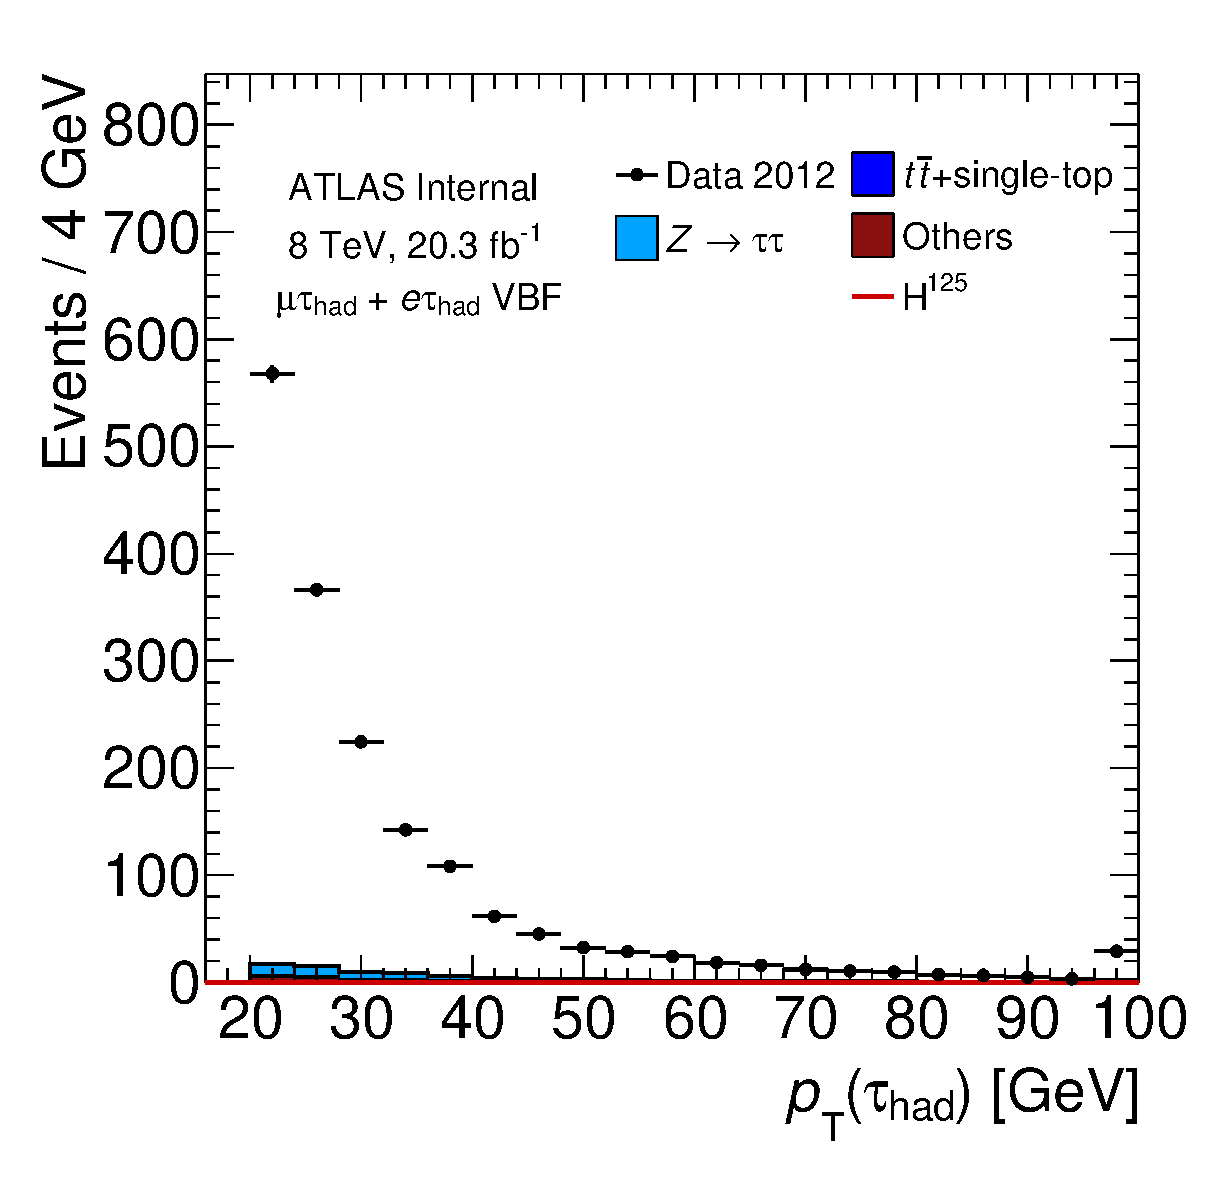
\includegraphics[width=0.32\textwidth]{figures/antitaus/tau-pt}
  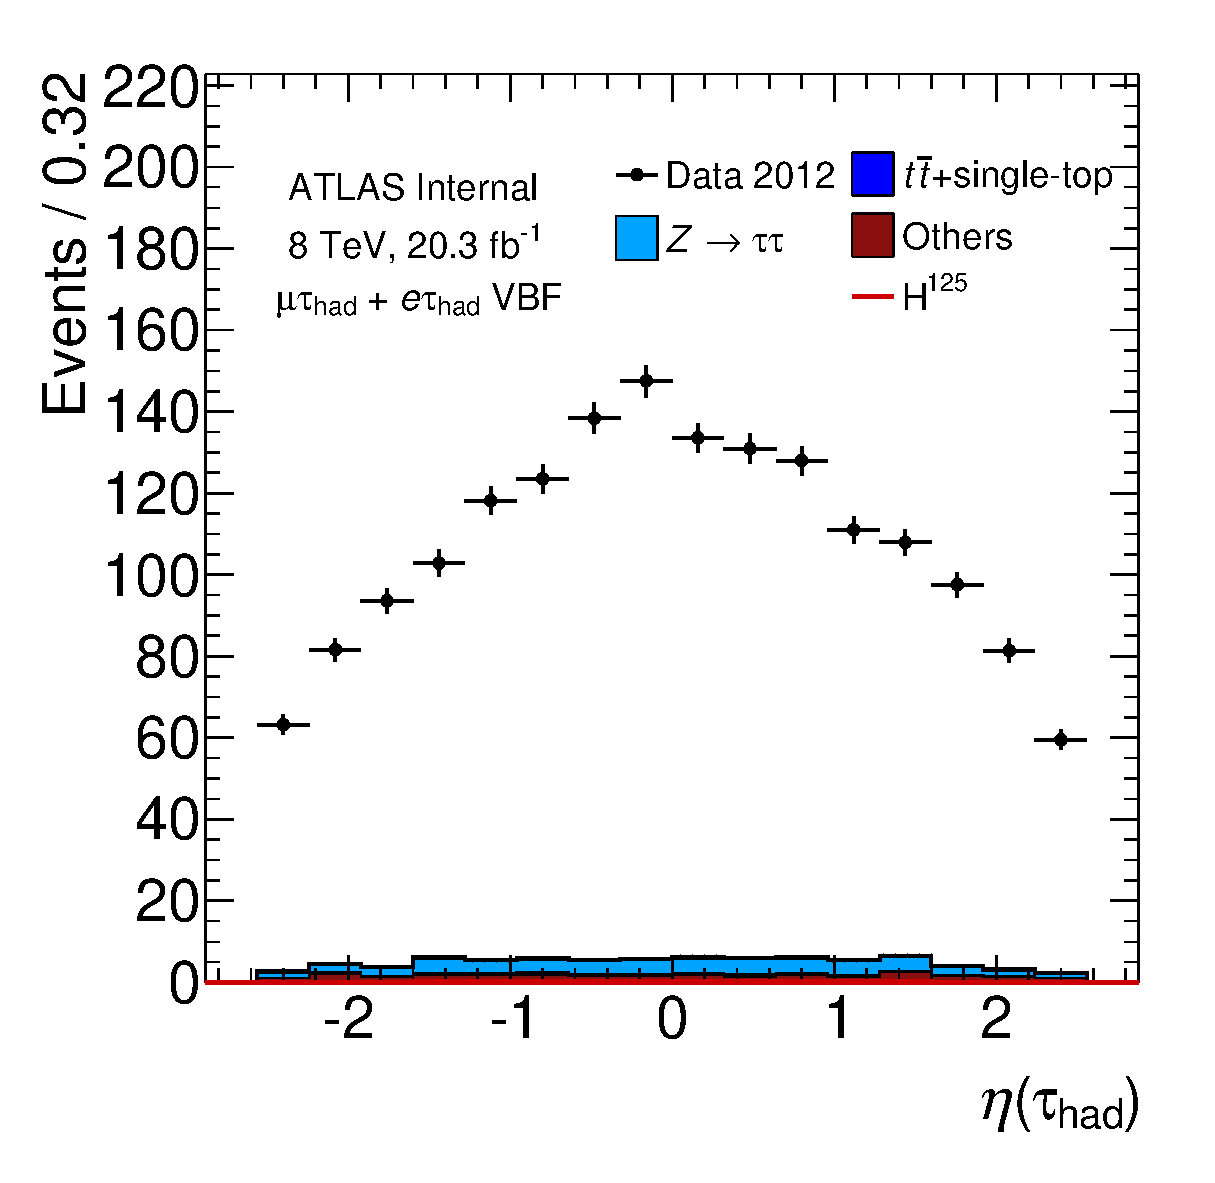
\includegraphics[width=0.32\textwidth]{figures/antitaus/tau-eta}
  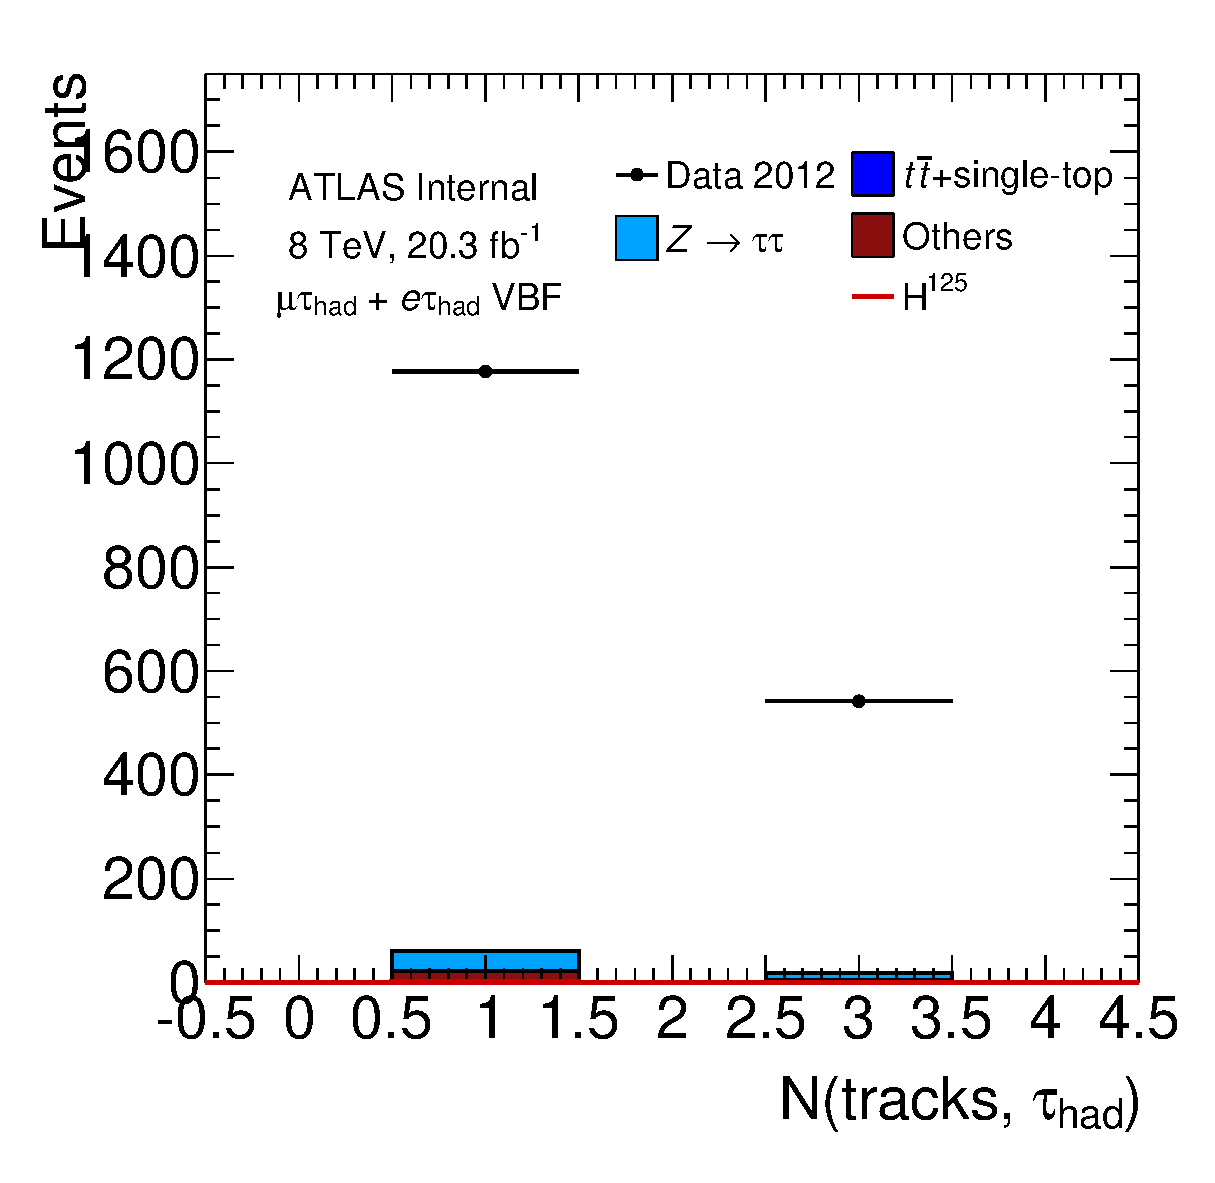
\includegraphics[width=0.32\textwidth]{figures/antitaus/tau-numTrack}
  % --------------
  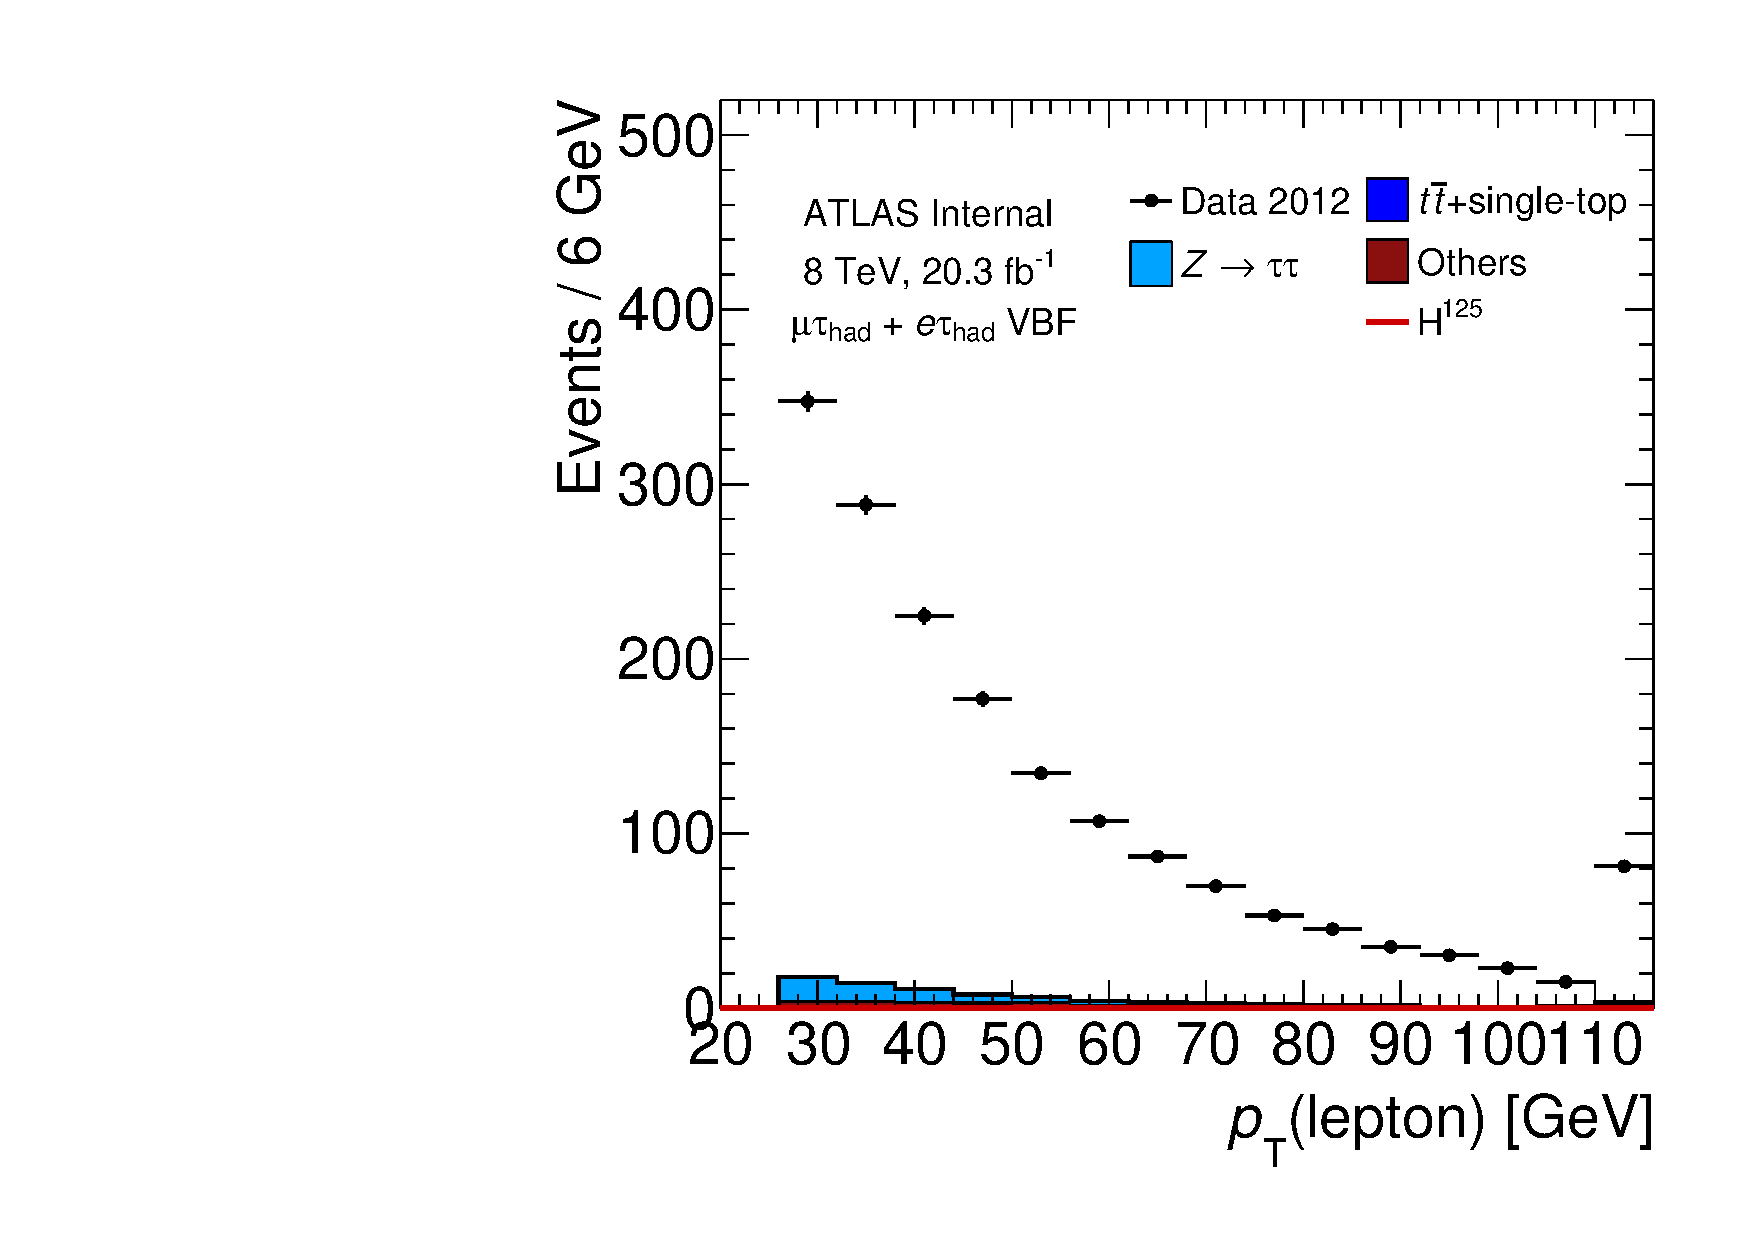
\includegraphics[width=0.32\textwidth]{figures/antitaus/lep-pt-hi}
  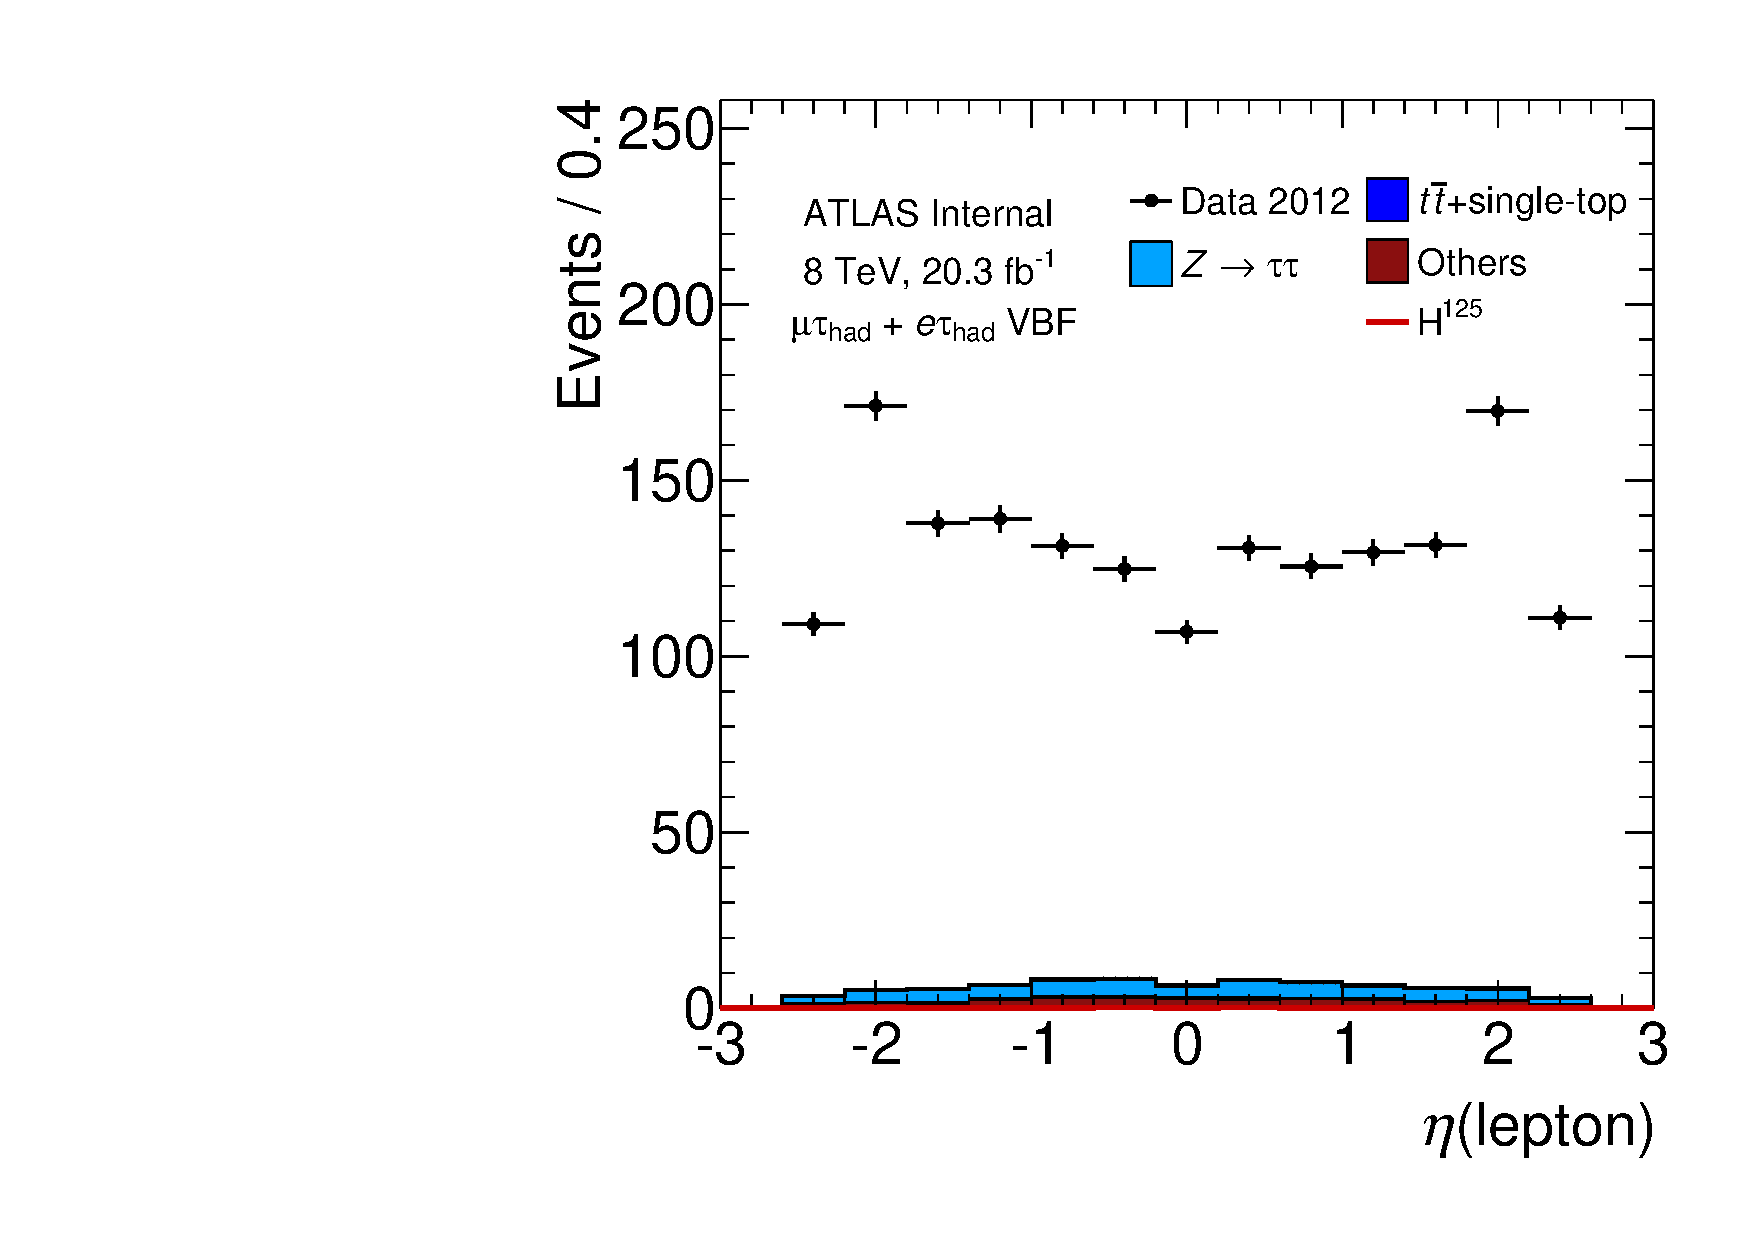
\includegraphics[width=0.32\textwidth]{figures/antitaus/lep-eta}
  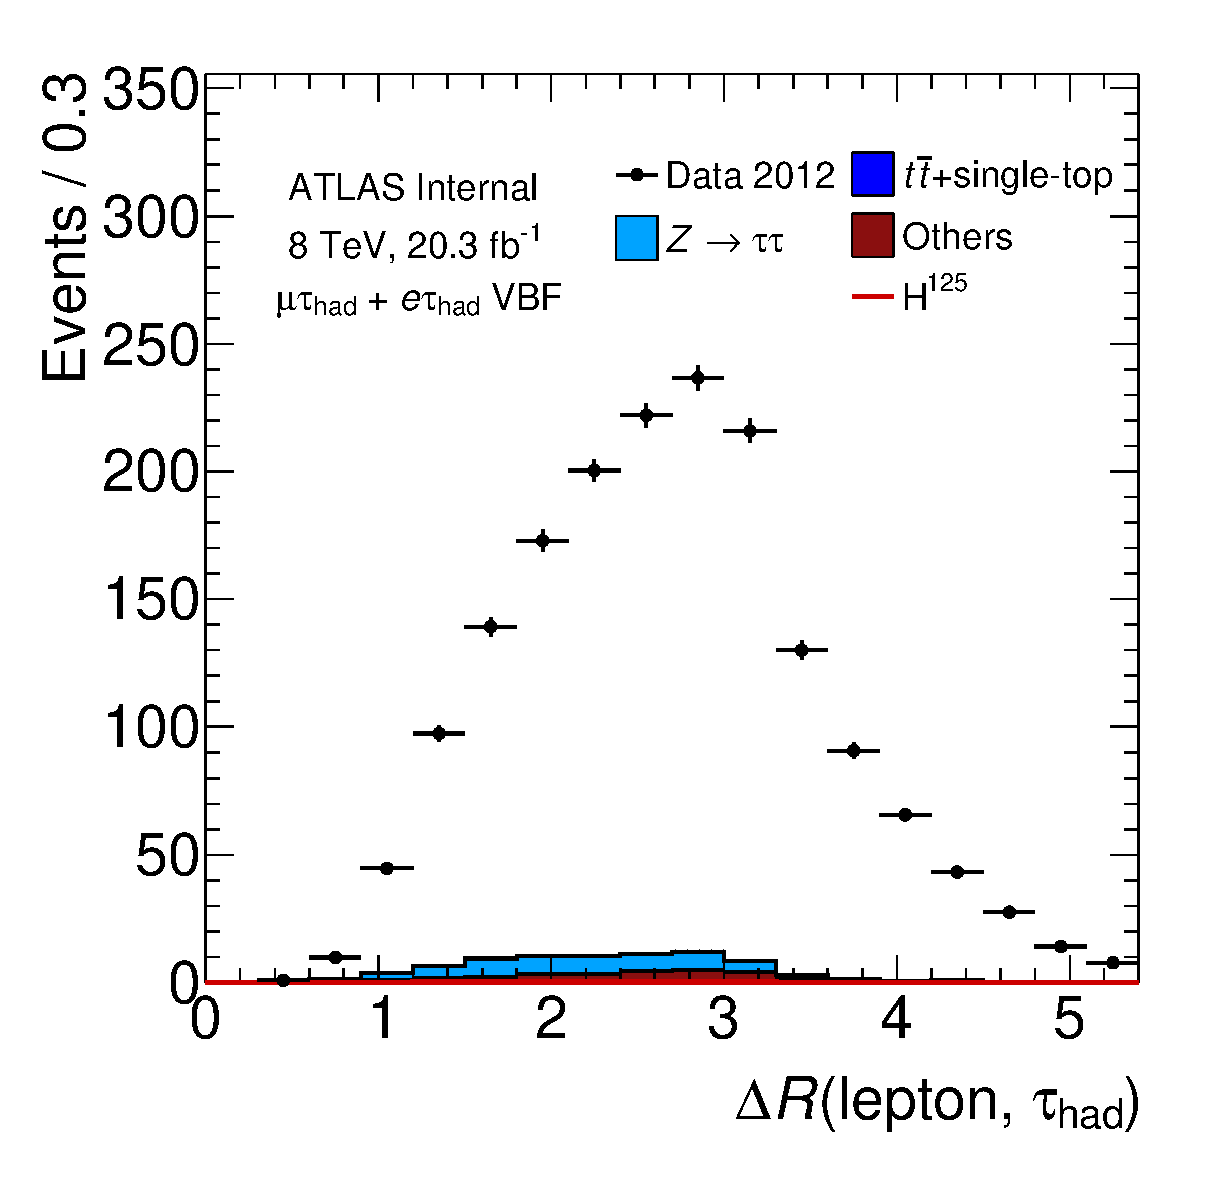
\includegraphics[width=0.32\textwidth]{figures/antitaus/taulep-dR}
  % --------------
  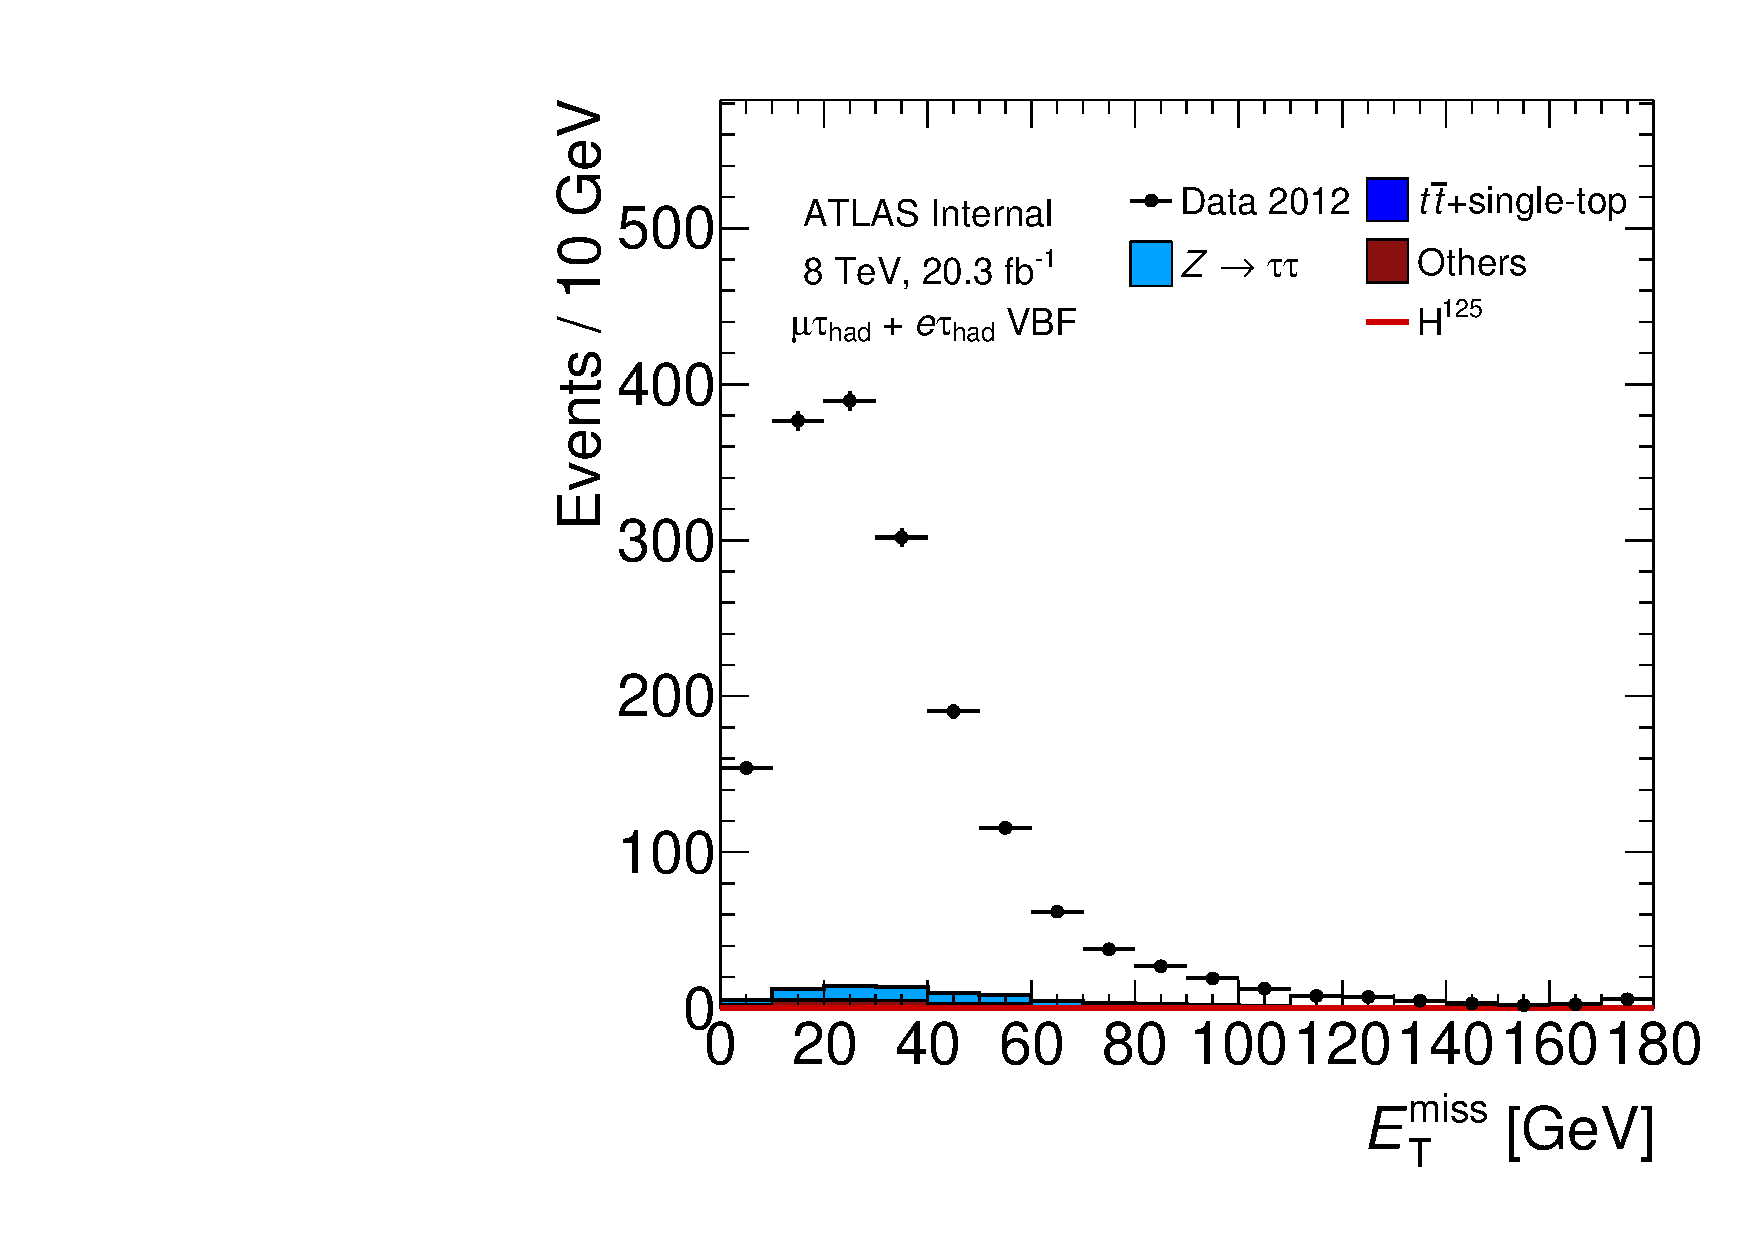
\includegraphics[width=0.32\textwidth]{figures/antitaus/met-pt-hi}
  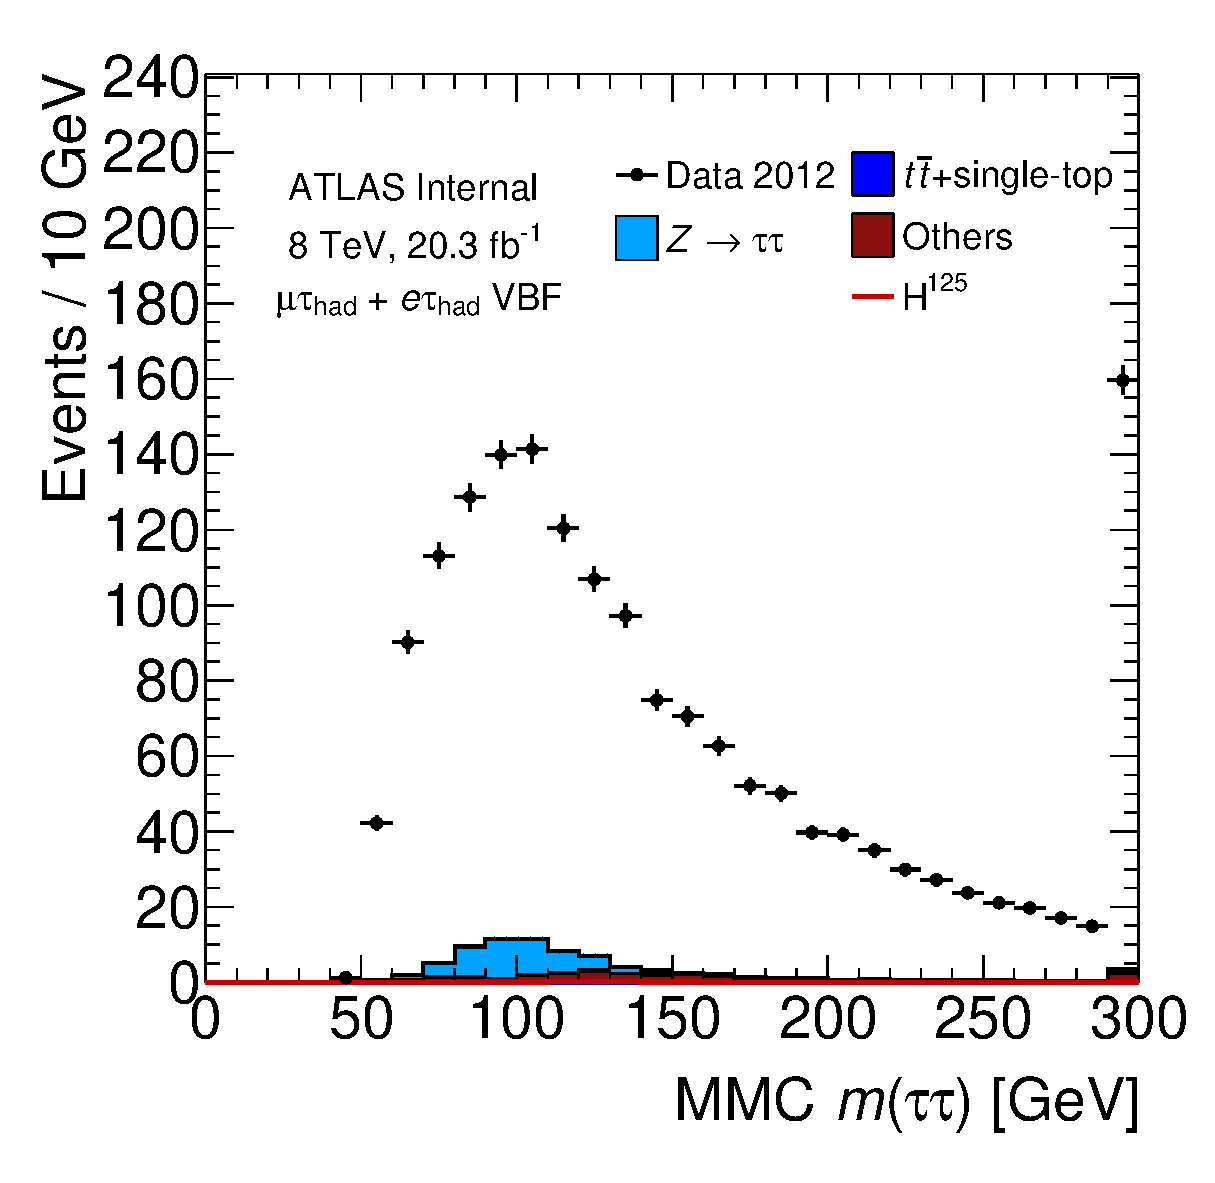
\includegraphics[width=0.32\textwidth]{figures/antitaus/mMMC}
  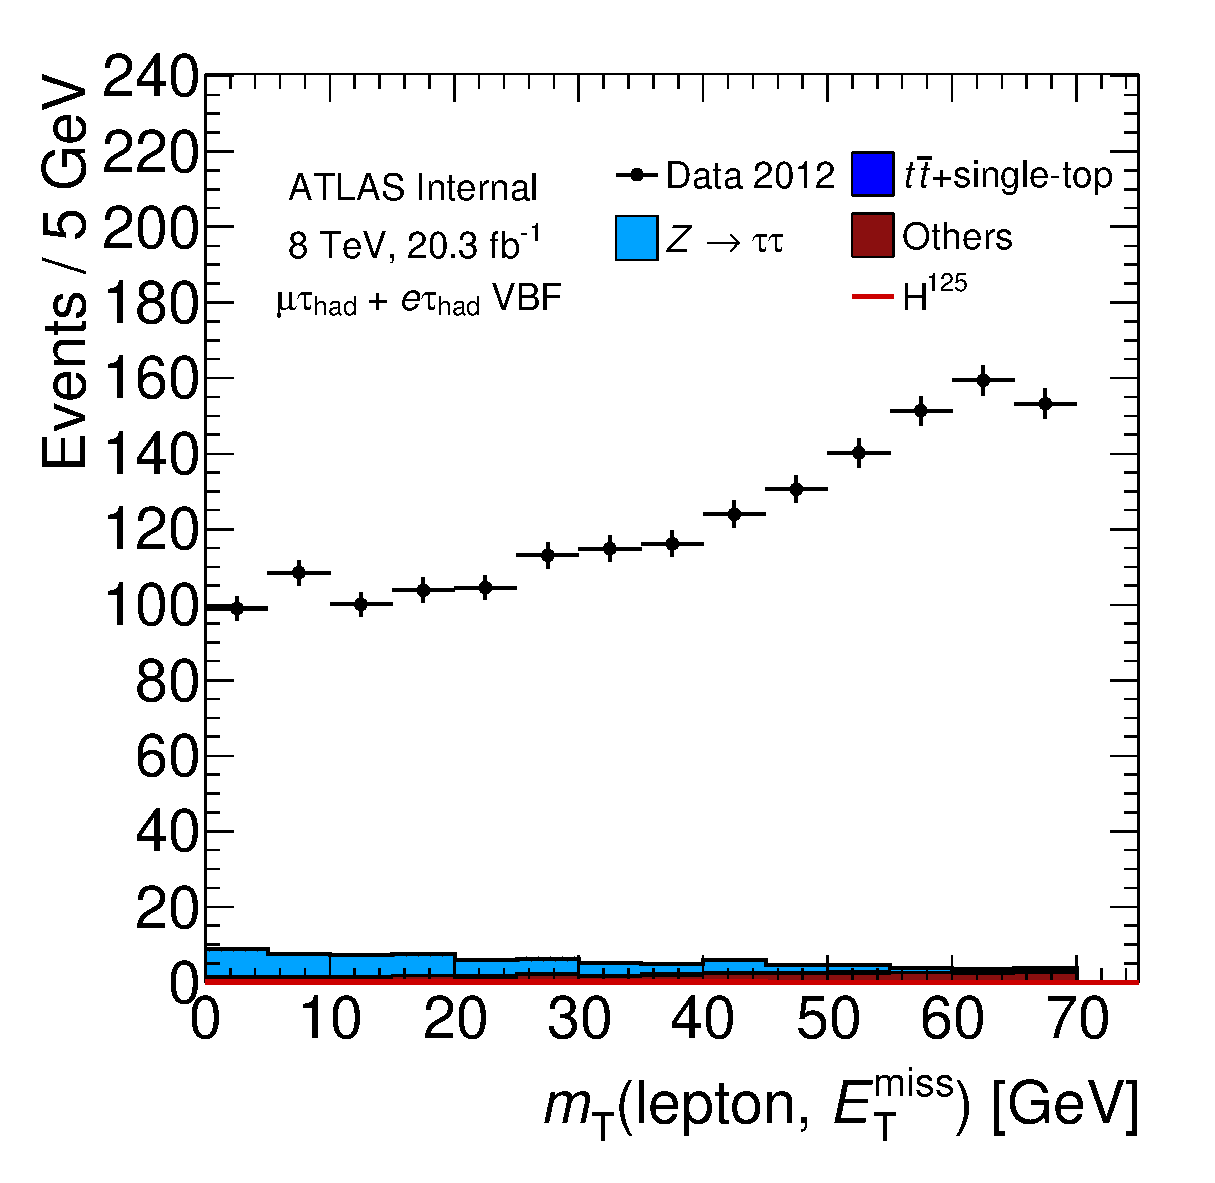
\includegraphics[width=0.32\textwidth]{figures/antitaus/mT}
  % --------------
  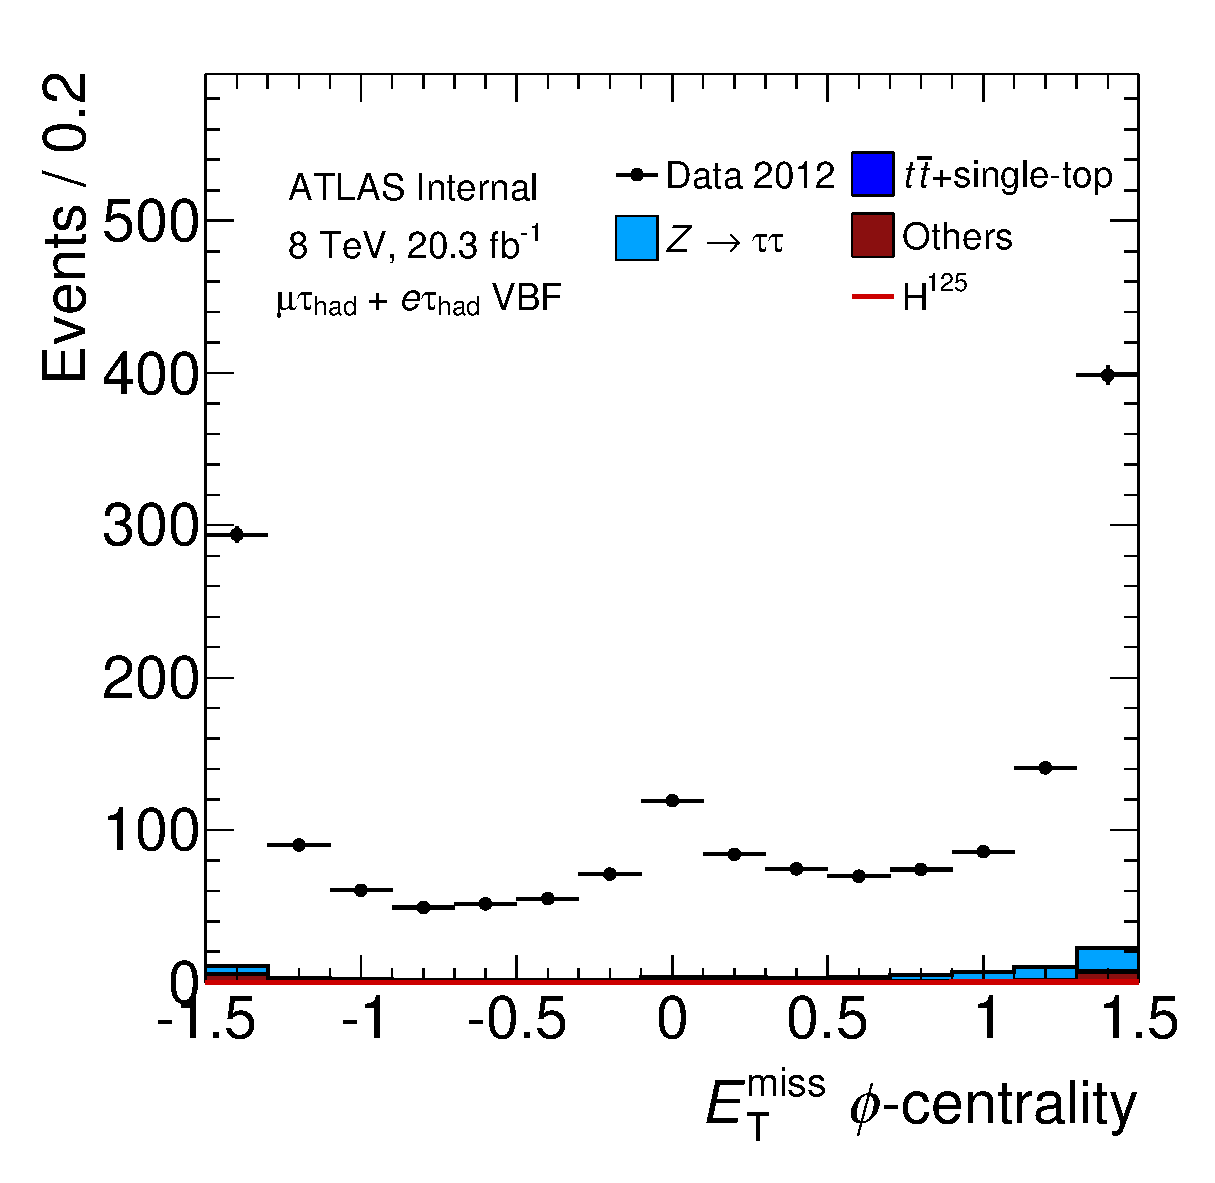
\includegraphics[width=0.32\textwidth]{figures/antitaus/met-phi-centrality}
  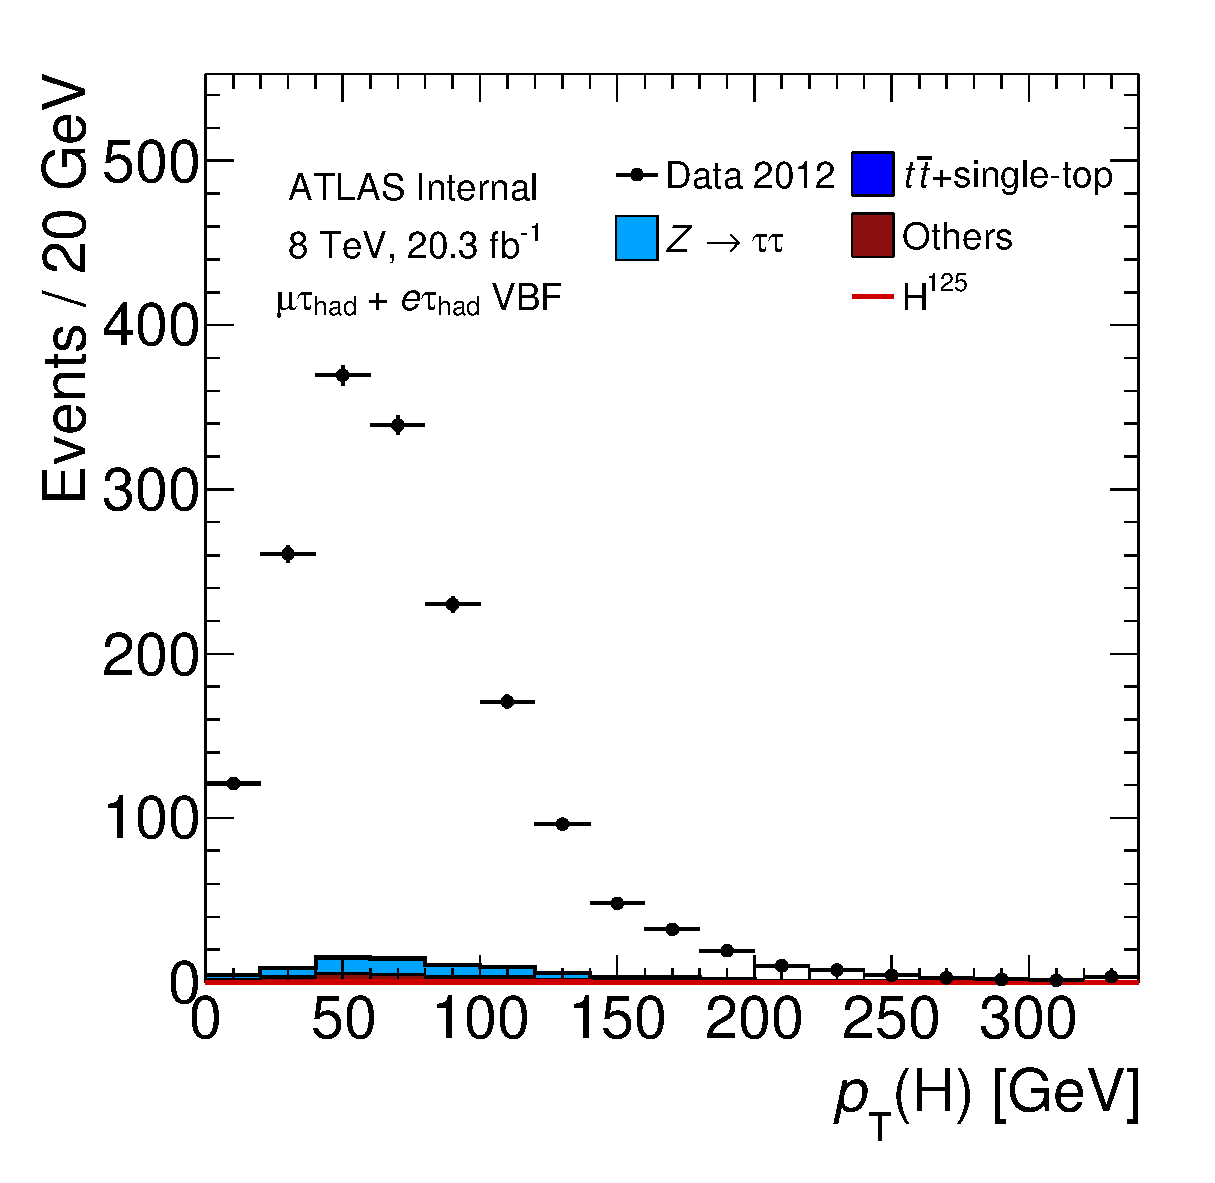
\includegraphics[width=0.32\textwidth]{figures/antitaus/H-pt-hi}
  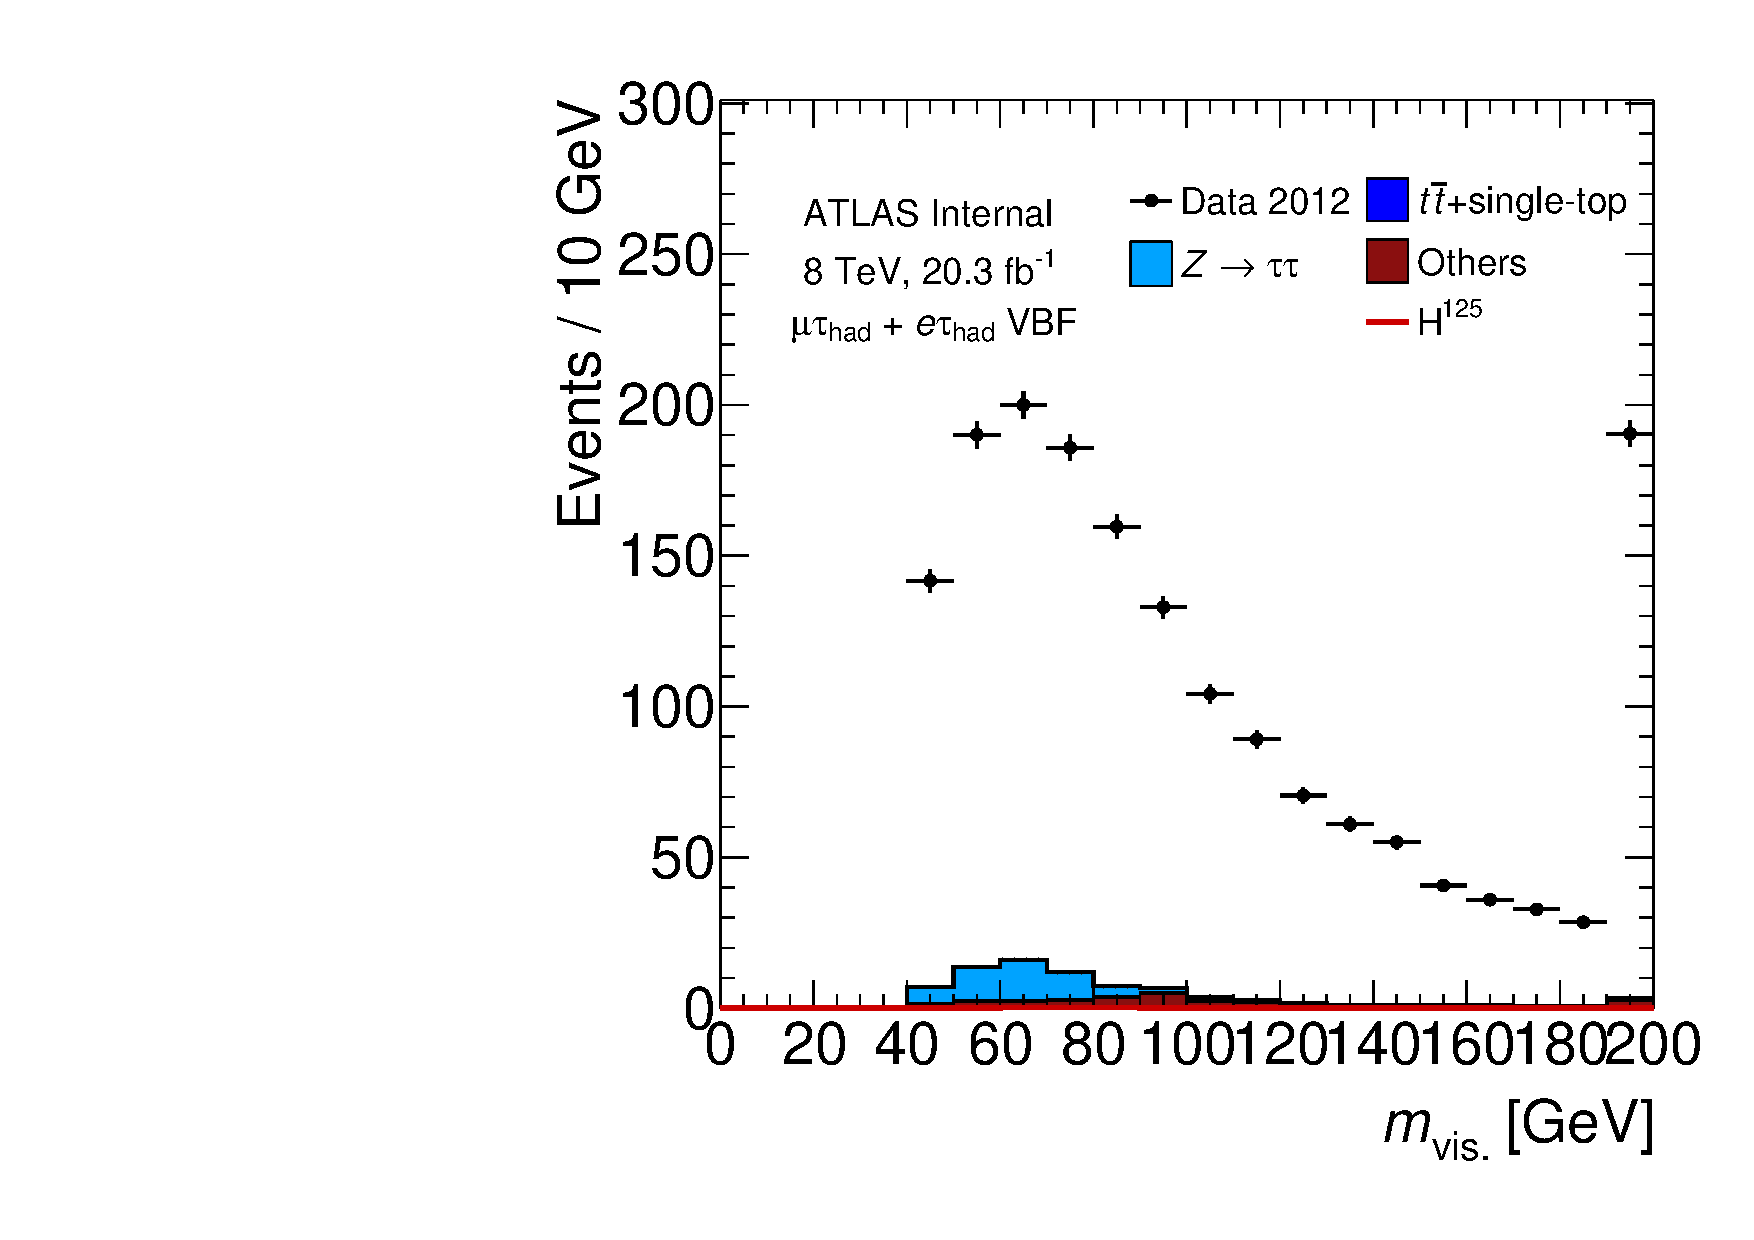
\includegraphics[width=0.32\textwidth]{figures/antitaus/mvis}
  \caption{Data events in the VBF category which fail $\tauh$ identification but fulfill all other requirements. The contamination of $\Ztautaulh$ and other processes without $\fakes$ is less than 10\%.}
  \label{fig:backgrounds-antitaus-taus}
\end{figure}

\clearpage

\begin{figure}[tp]
  \centering
  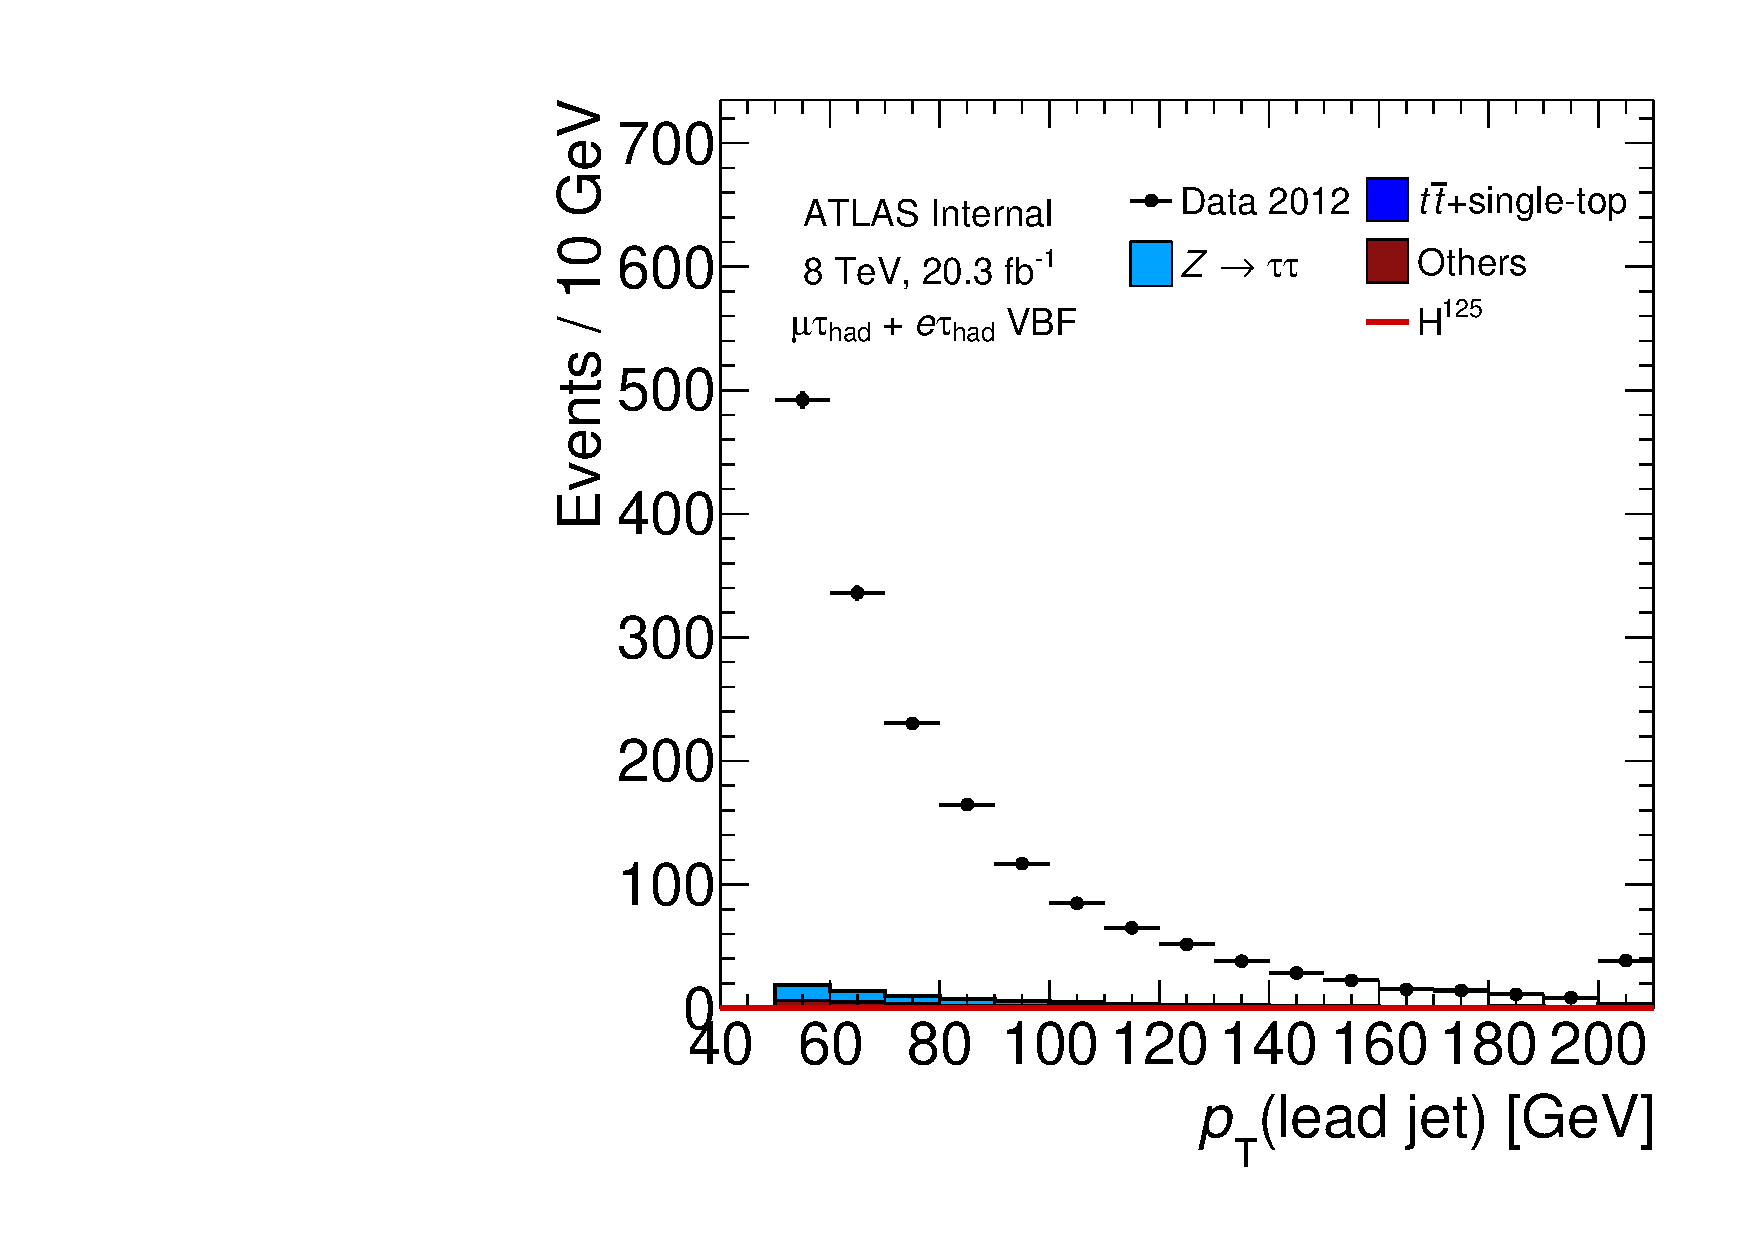
\includegraphics[width=0.32\textwidth]{figures/antitaus/jet-1-pt}
  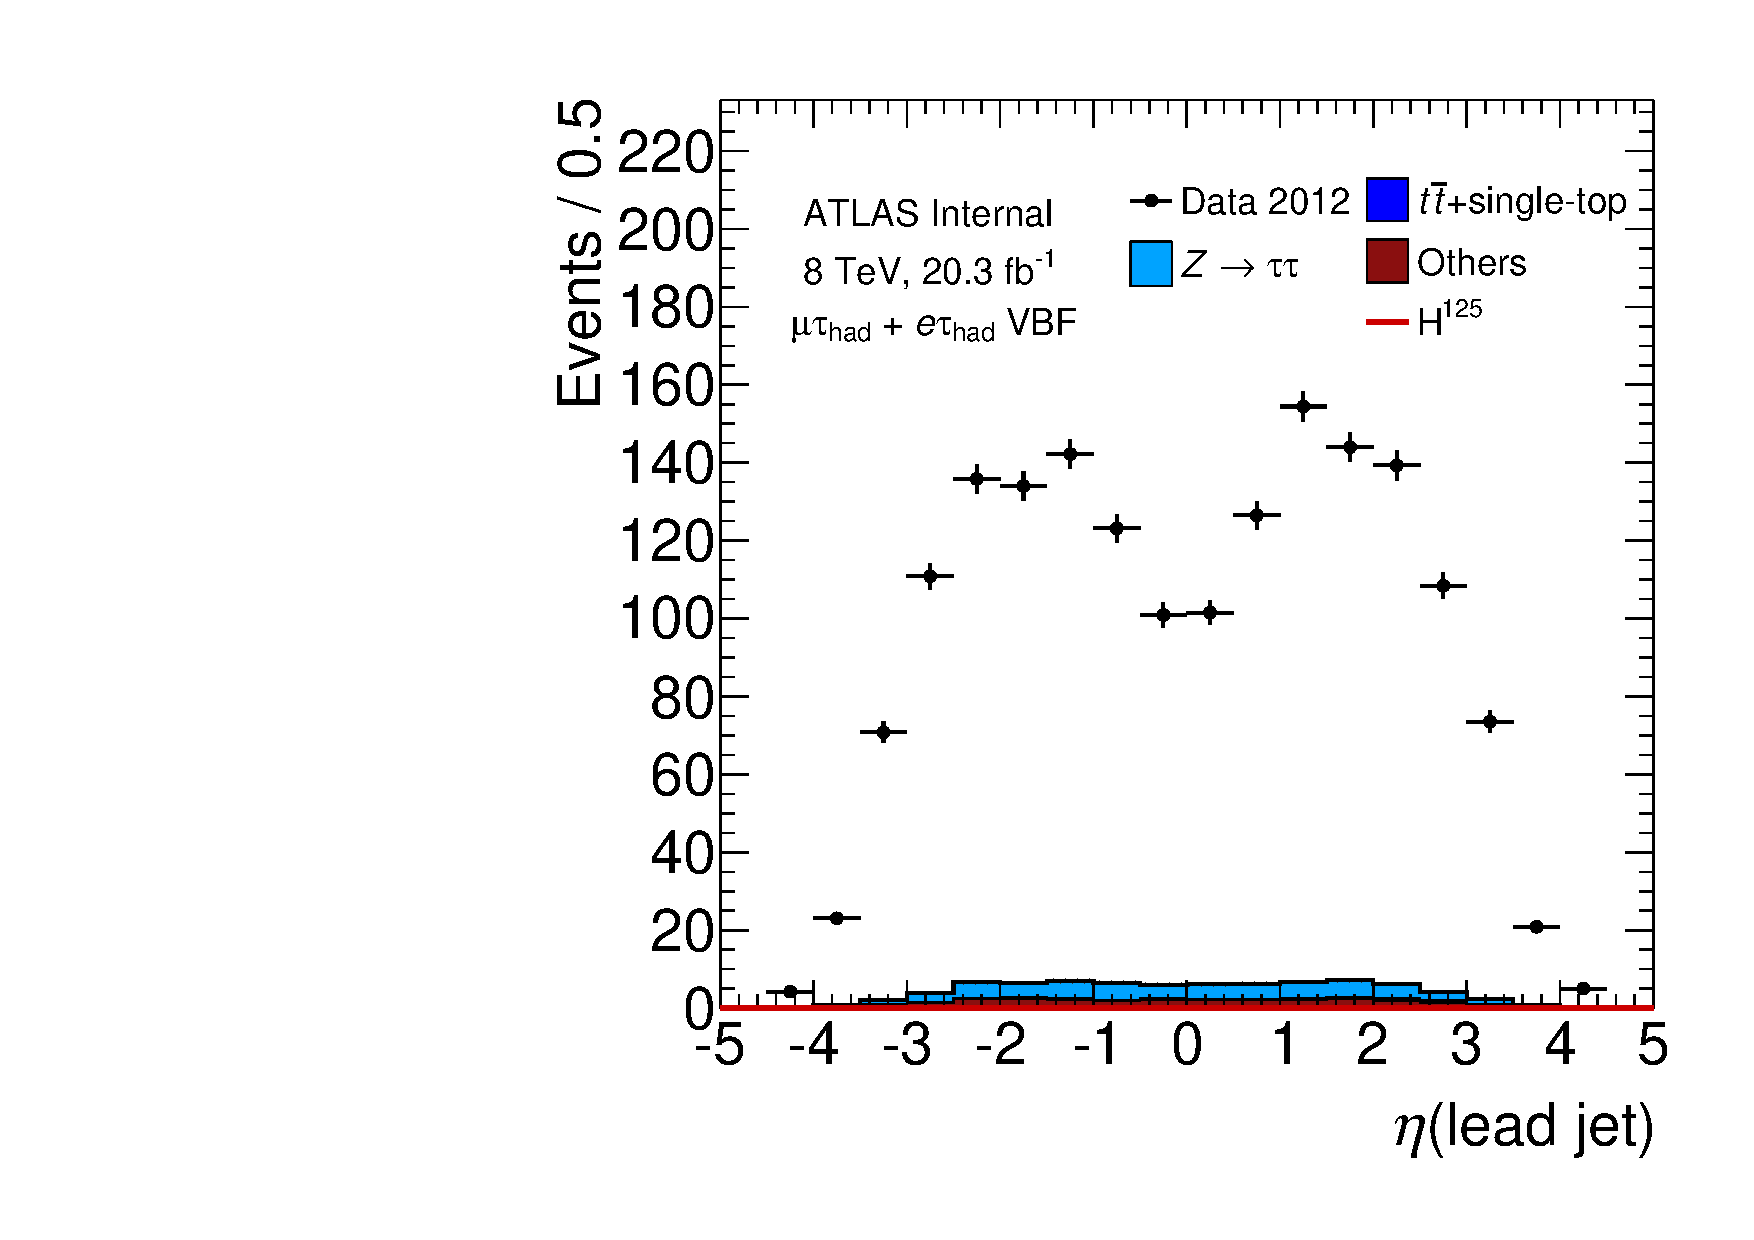
\includegraphics[width=0.32\textwidth]{figures/antitaus/jet-1-eta}
  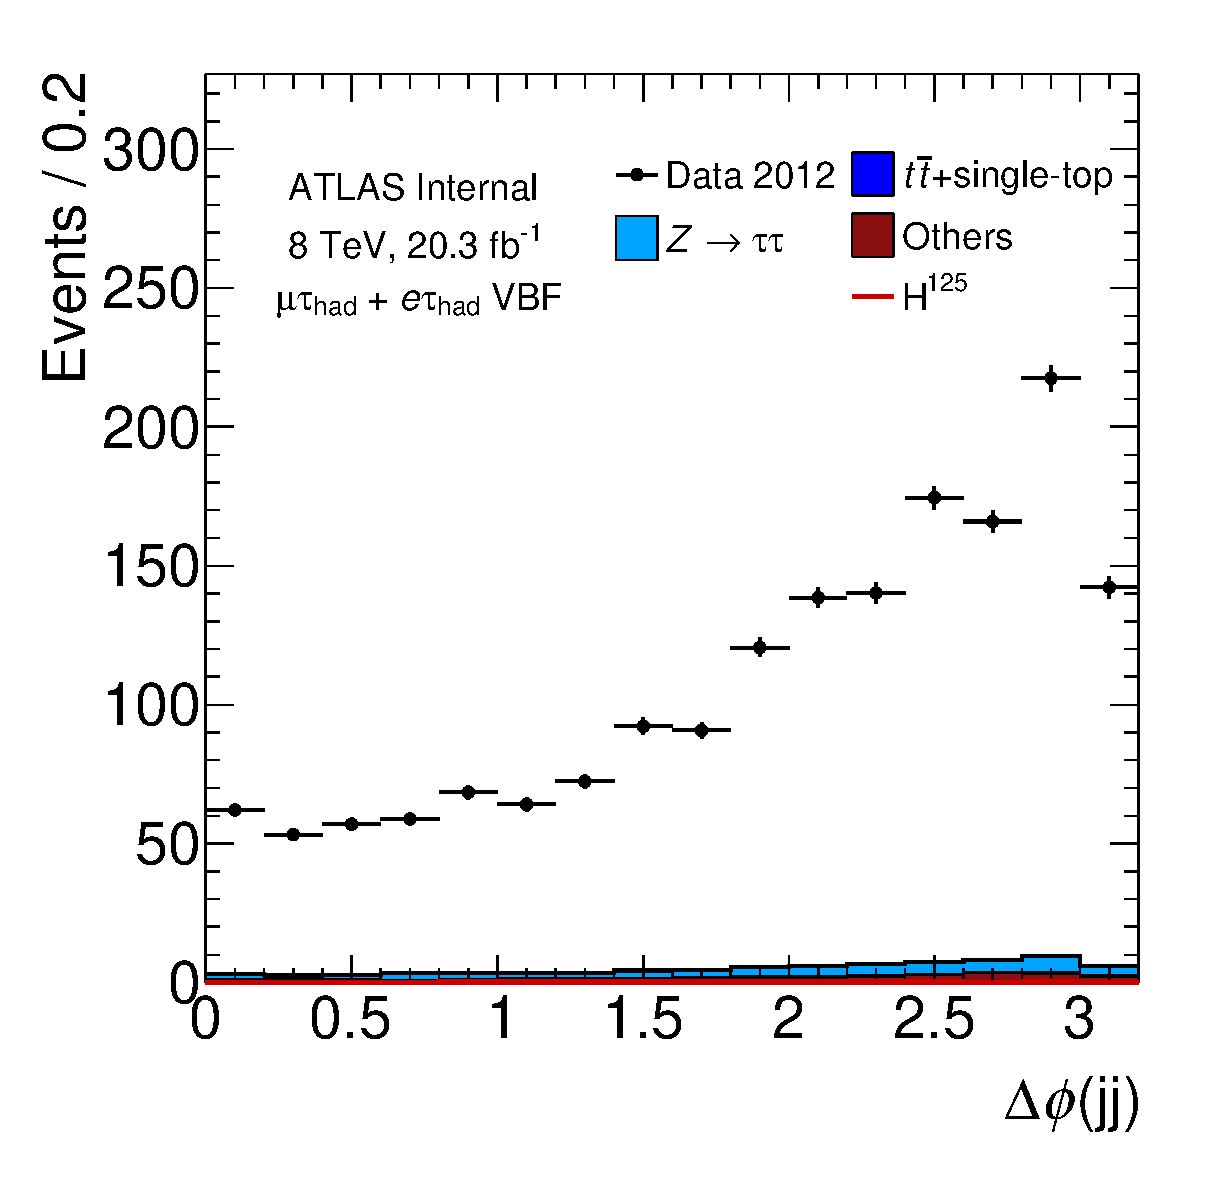
\includegraphics[width=0.32\textwidth]{figures/antitaus/jets-dphi}
  % --------------
  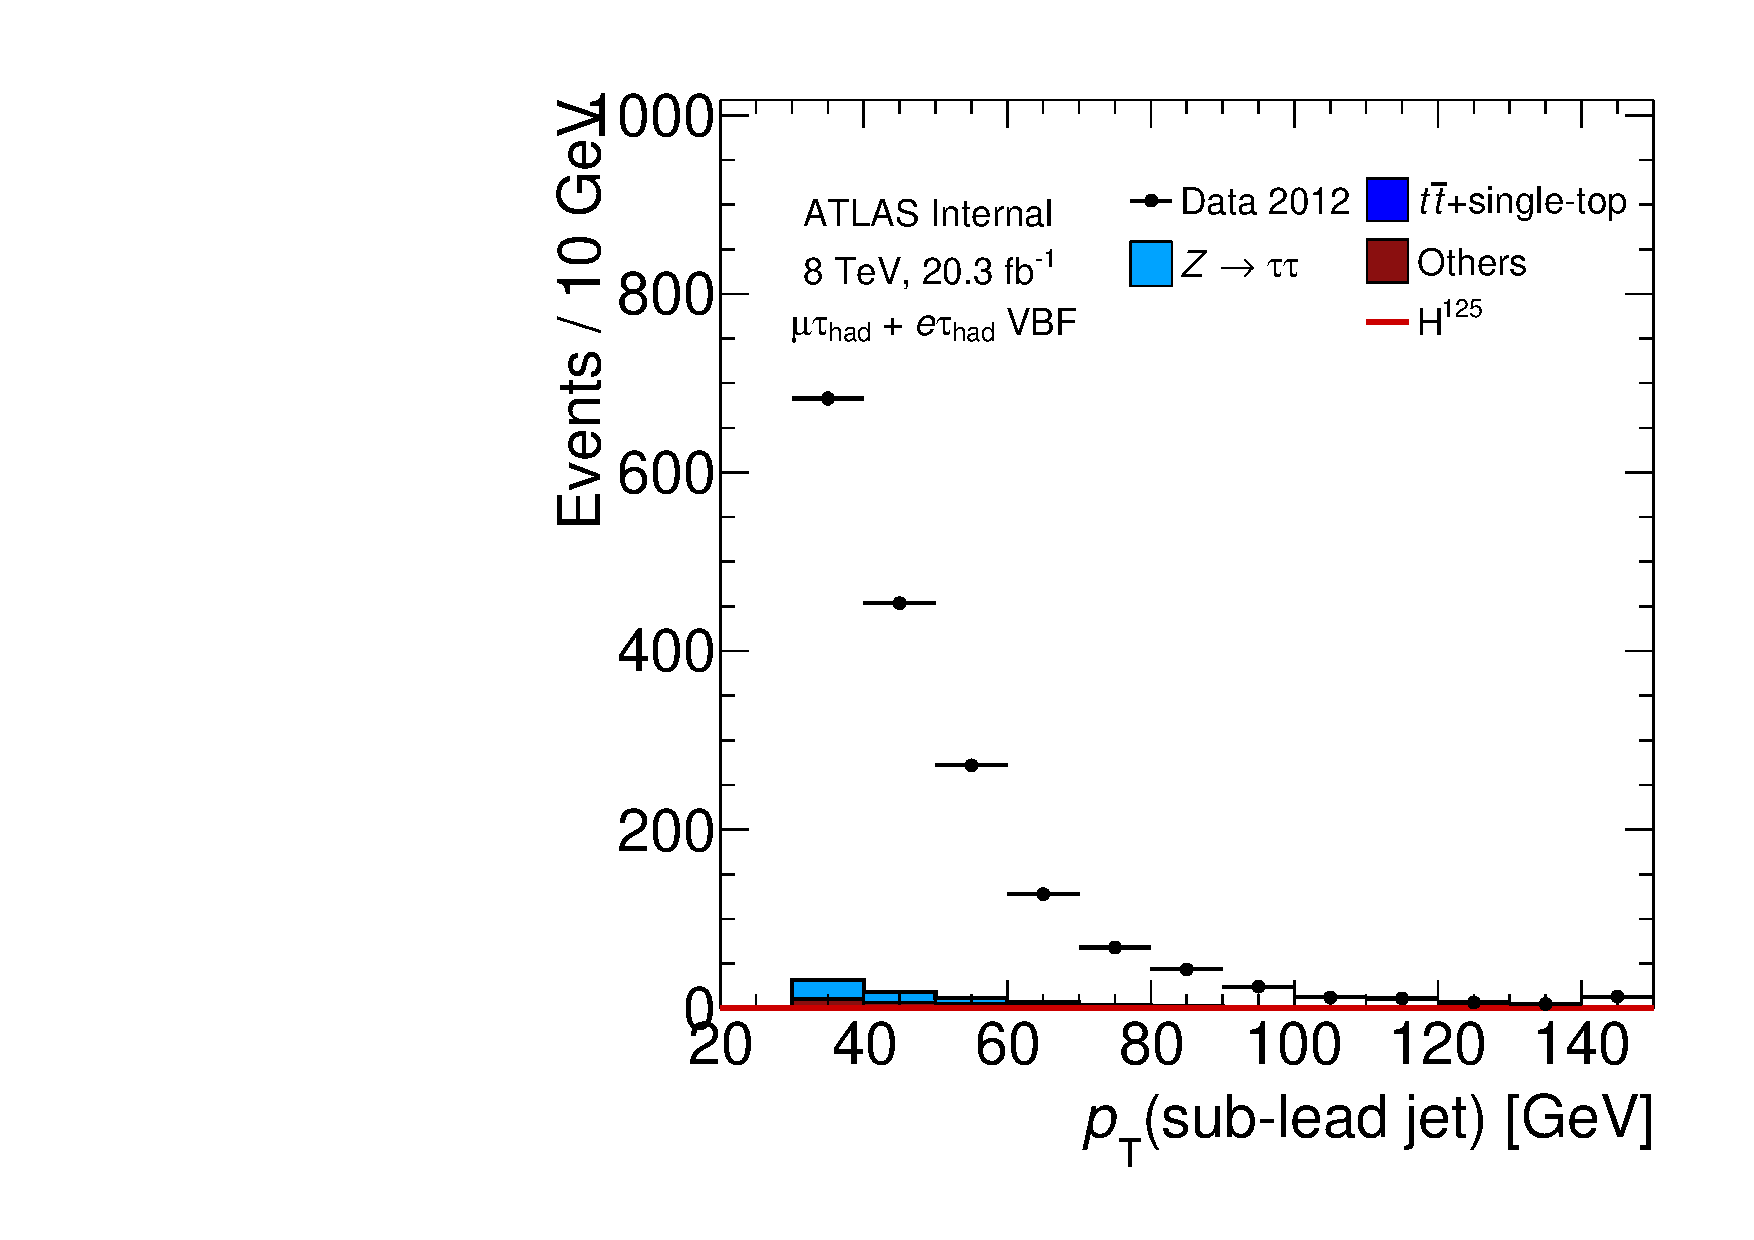
\includegraphics[width=0.32\textwidth]{figures/antitaus/jet-2-pt}
  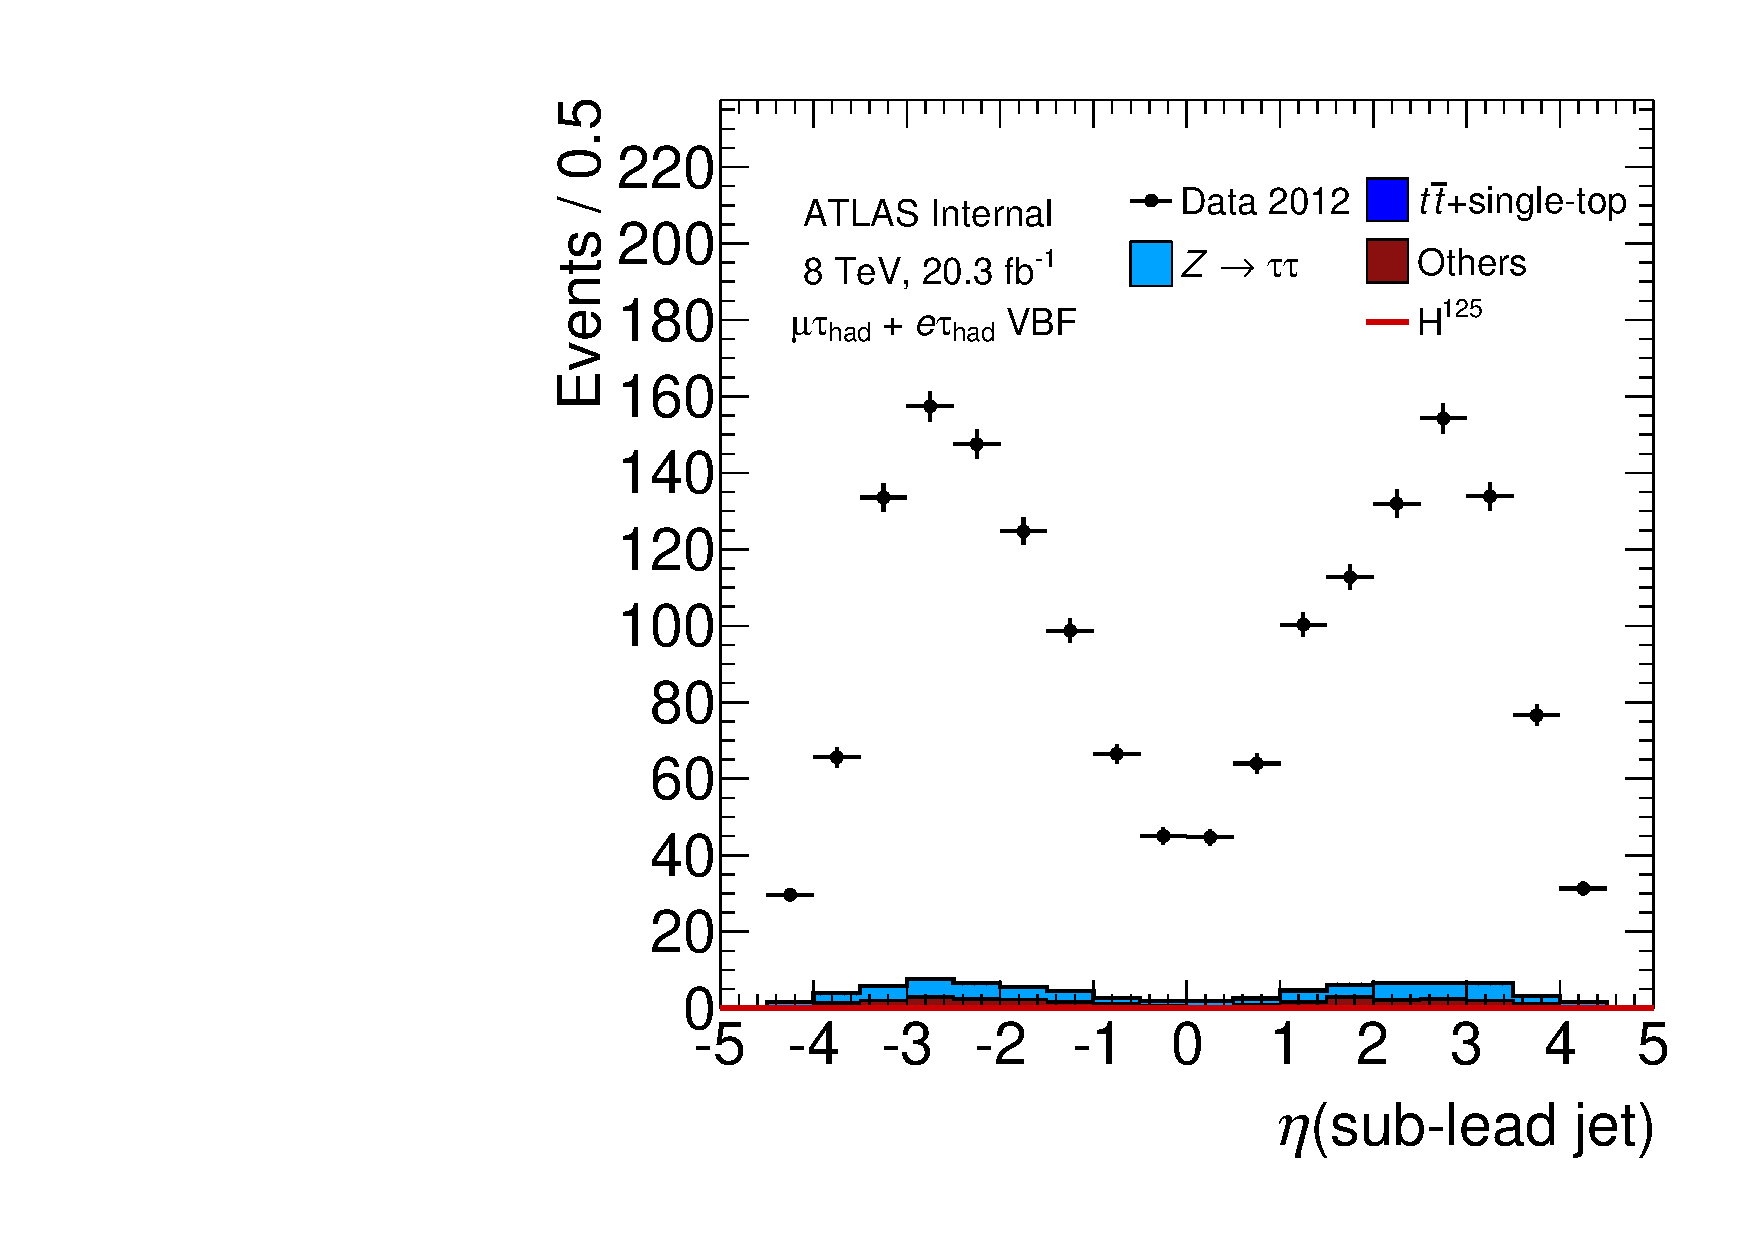
\includegraphics[width=0.32\textwidth]{figures/antitaus/jet-2-eta}
  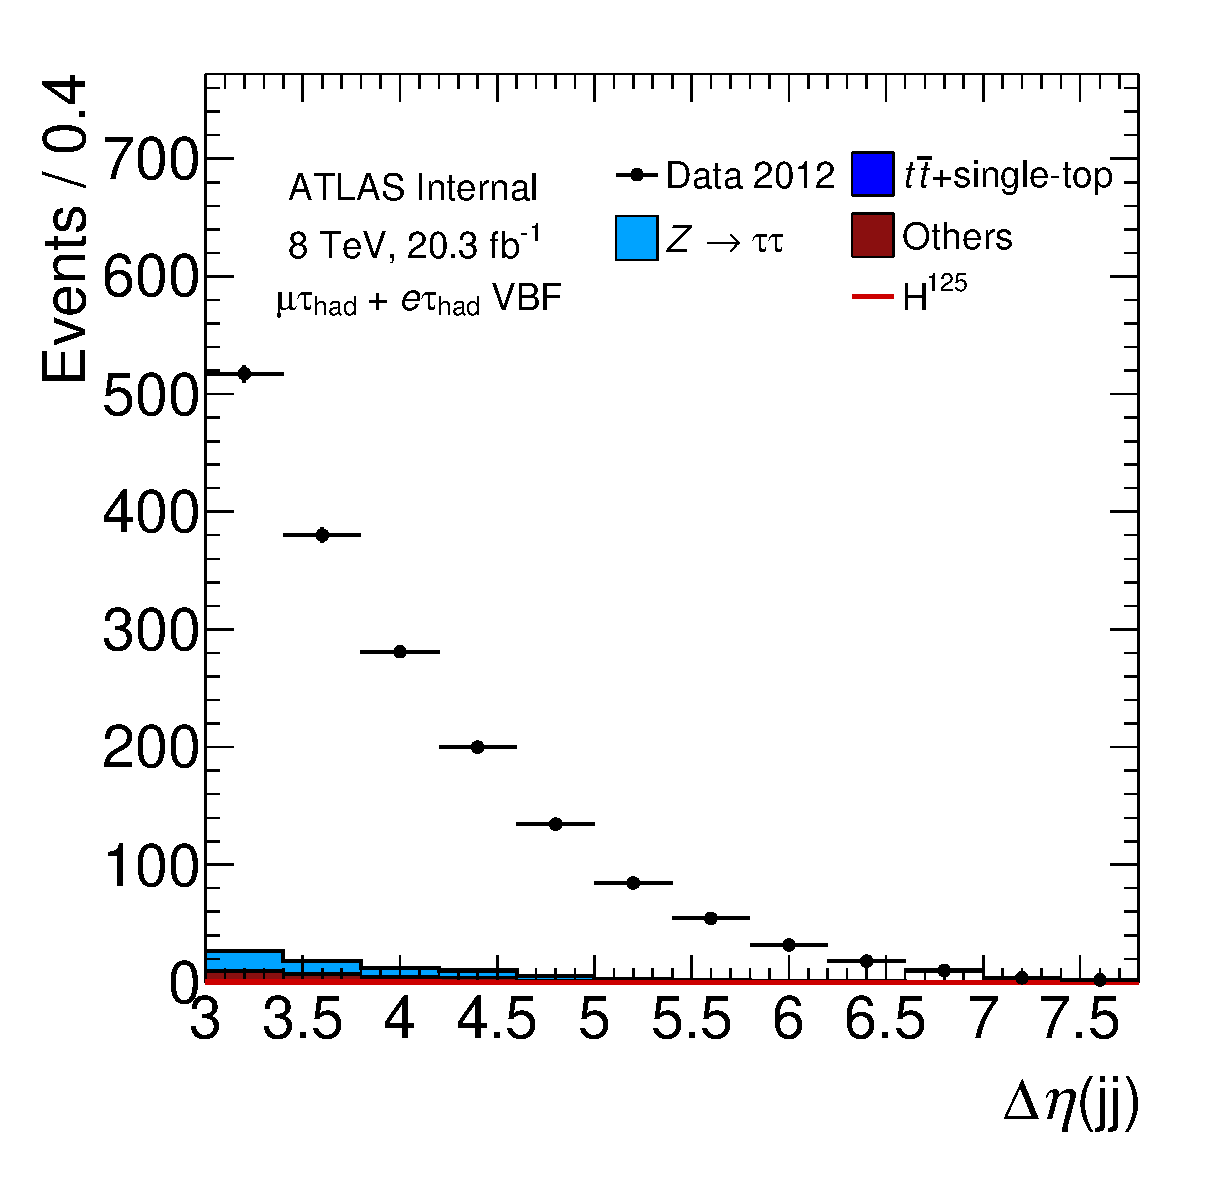
\includegraphics[width=0.32\textwidth]{figures/antitaus/jets-deta}
  % --------------
  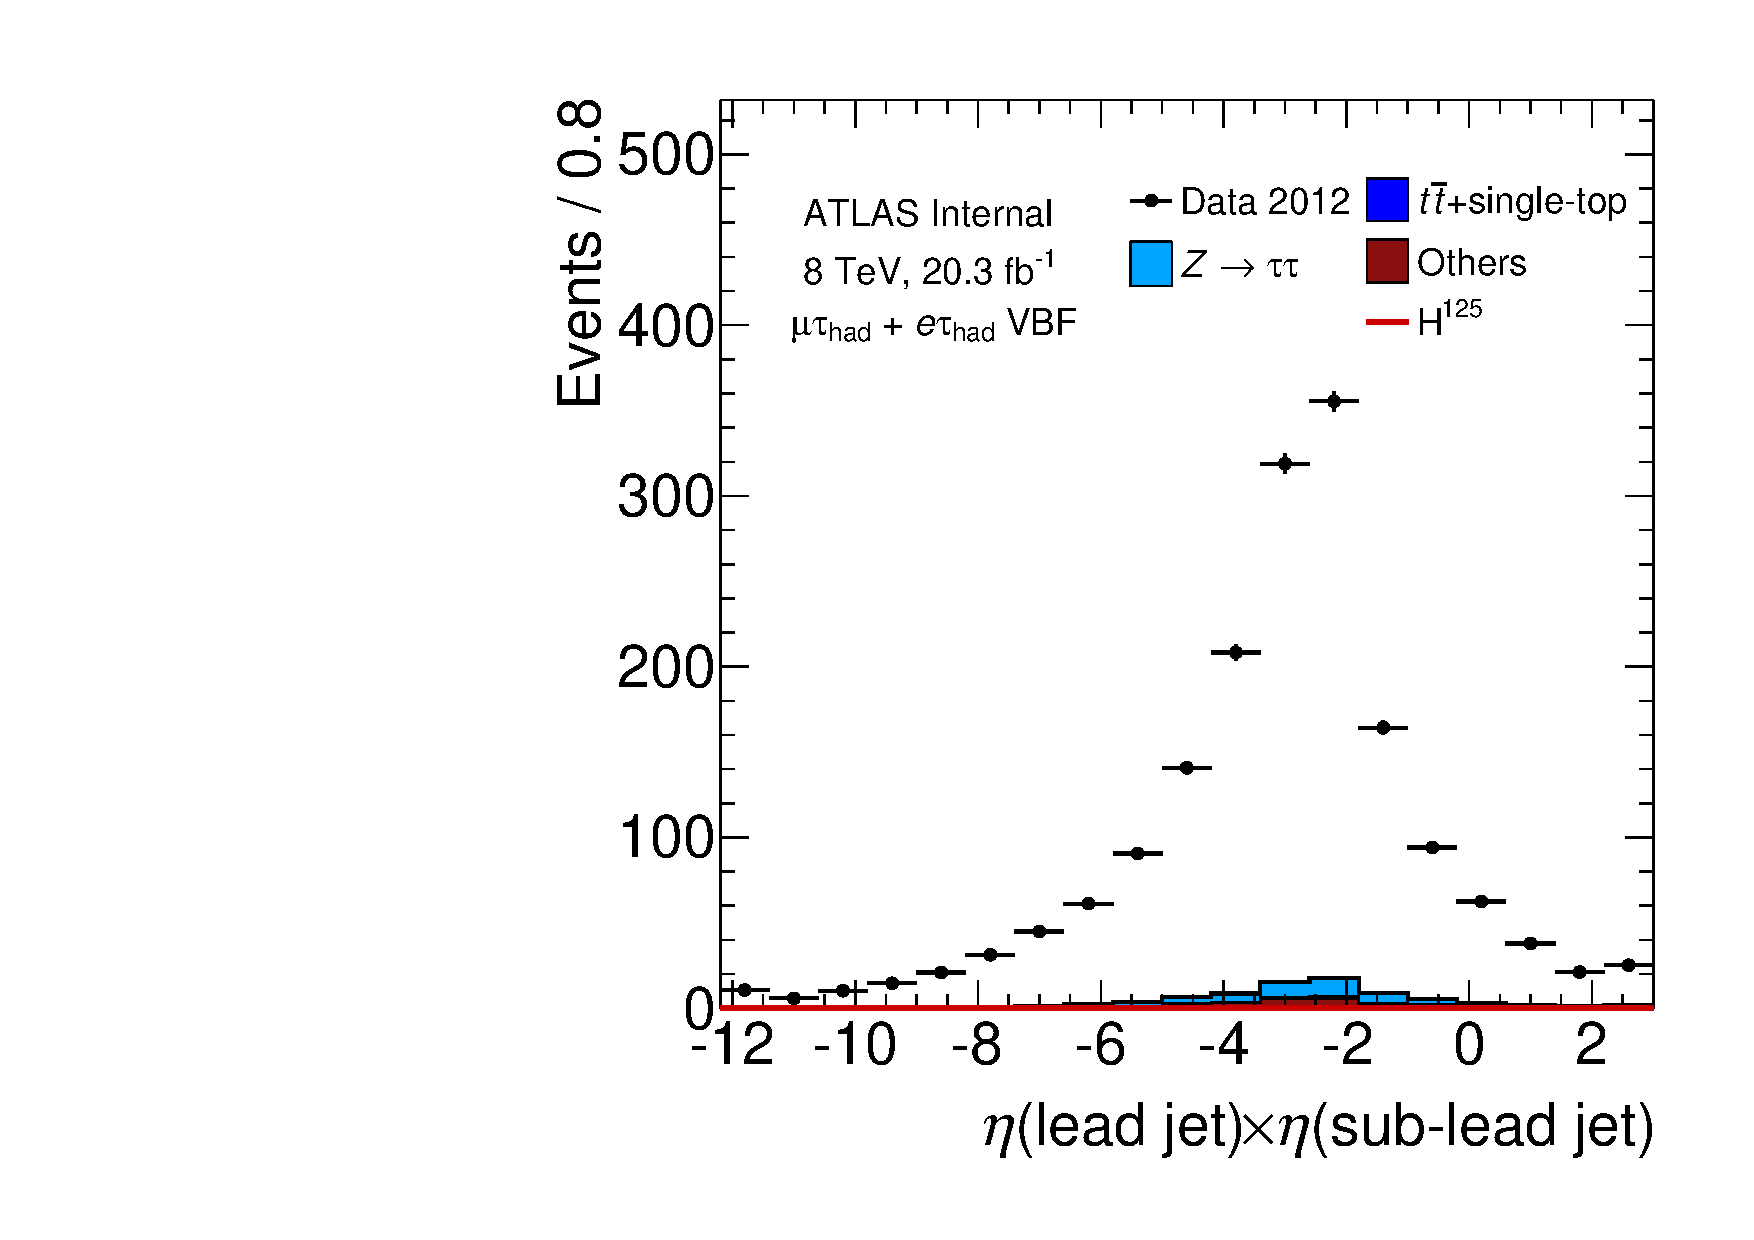
\includegraphics[width=0.32\textwidth]{figures/antitaus/jets-etaprod}
  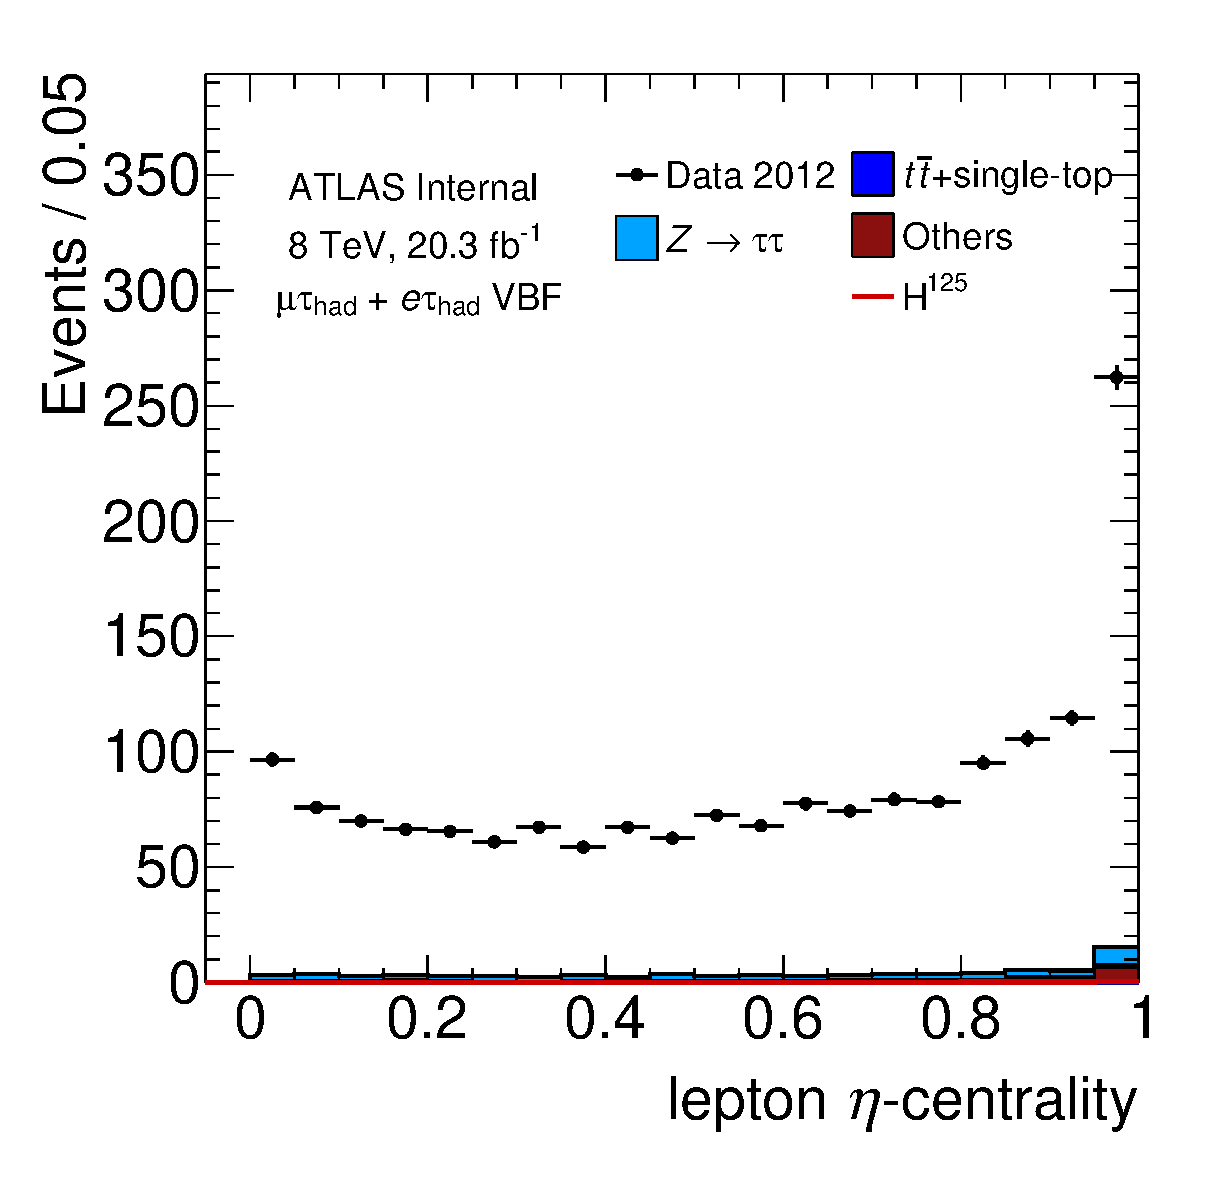
\includegraphics[width=0.32\textwidth]{figures/antitaus/lep-eta-centrality}
  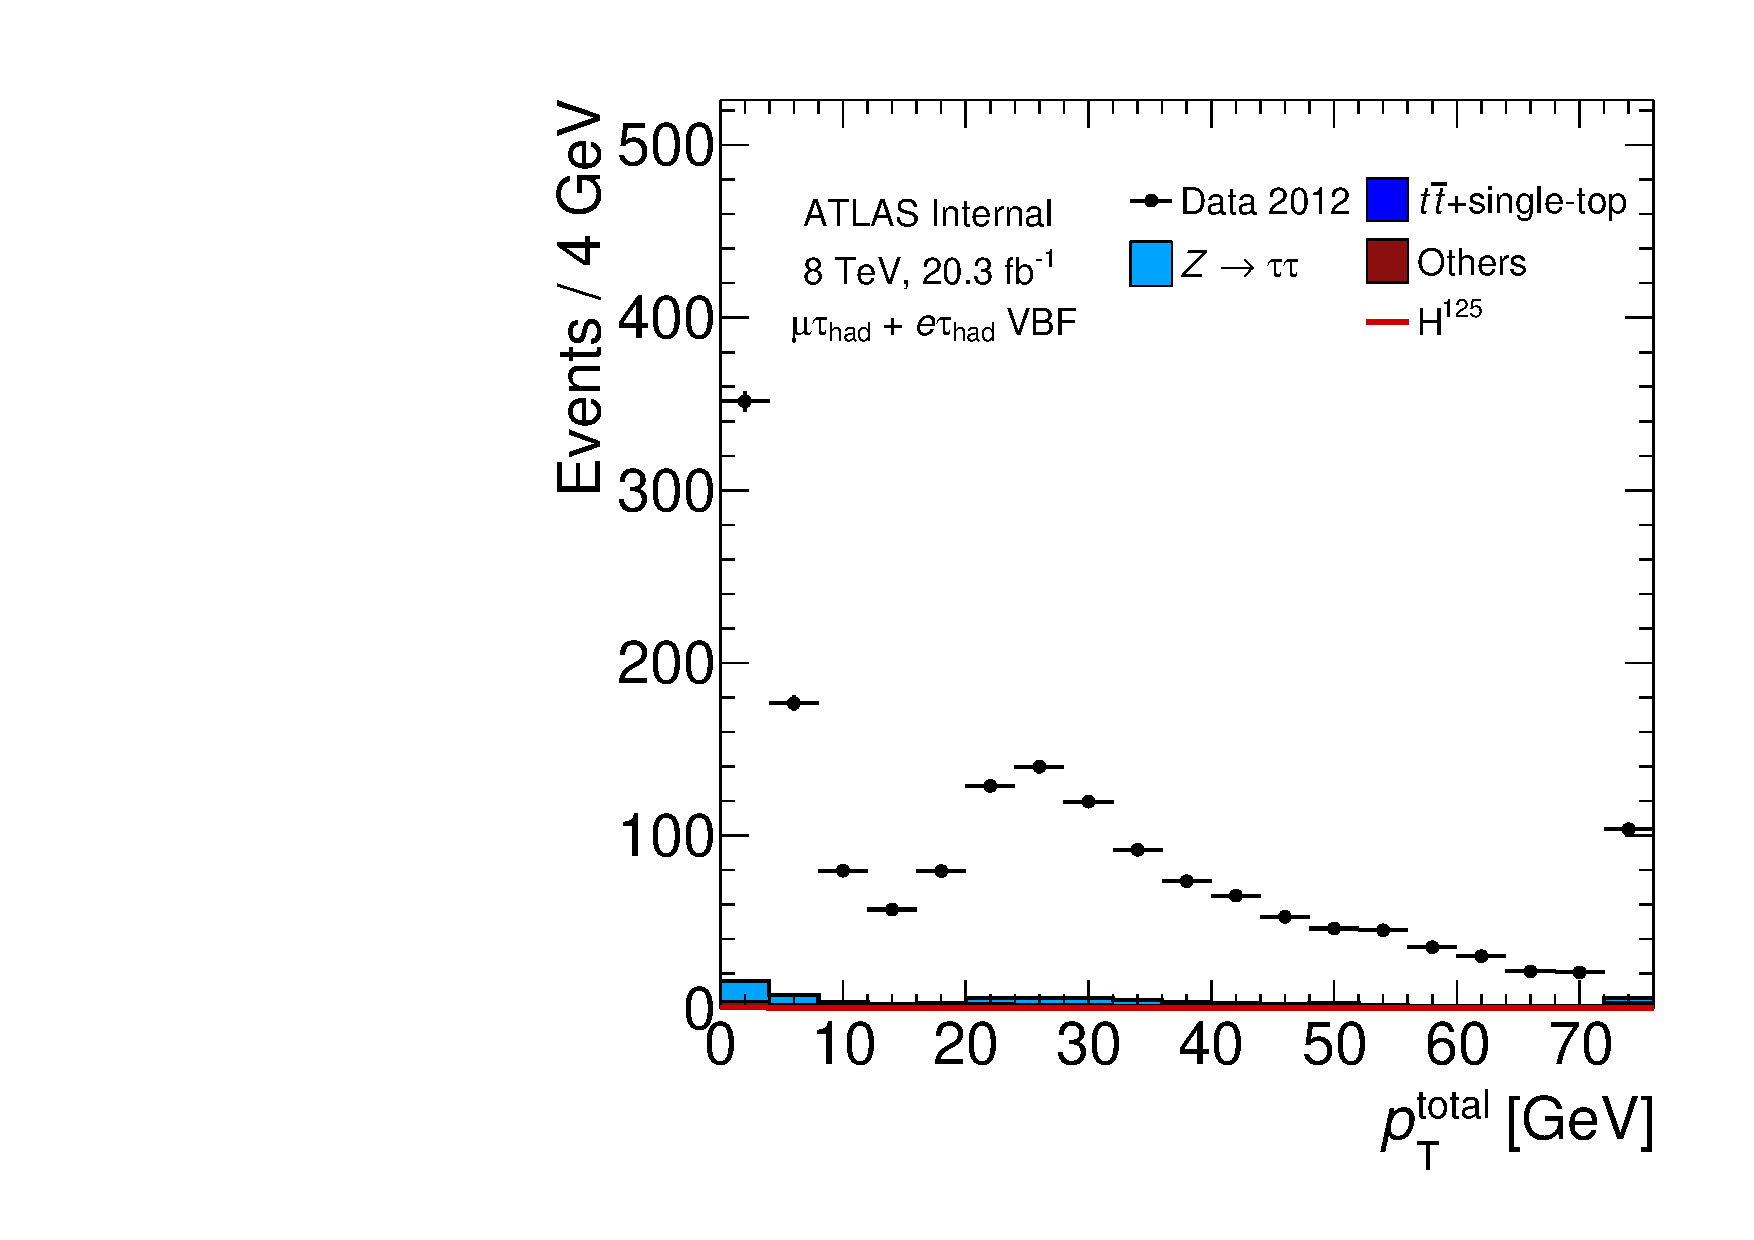
\includegraphics[width=0.32\textwidth]{figures/antitaus/system-pt}
  % --------------
  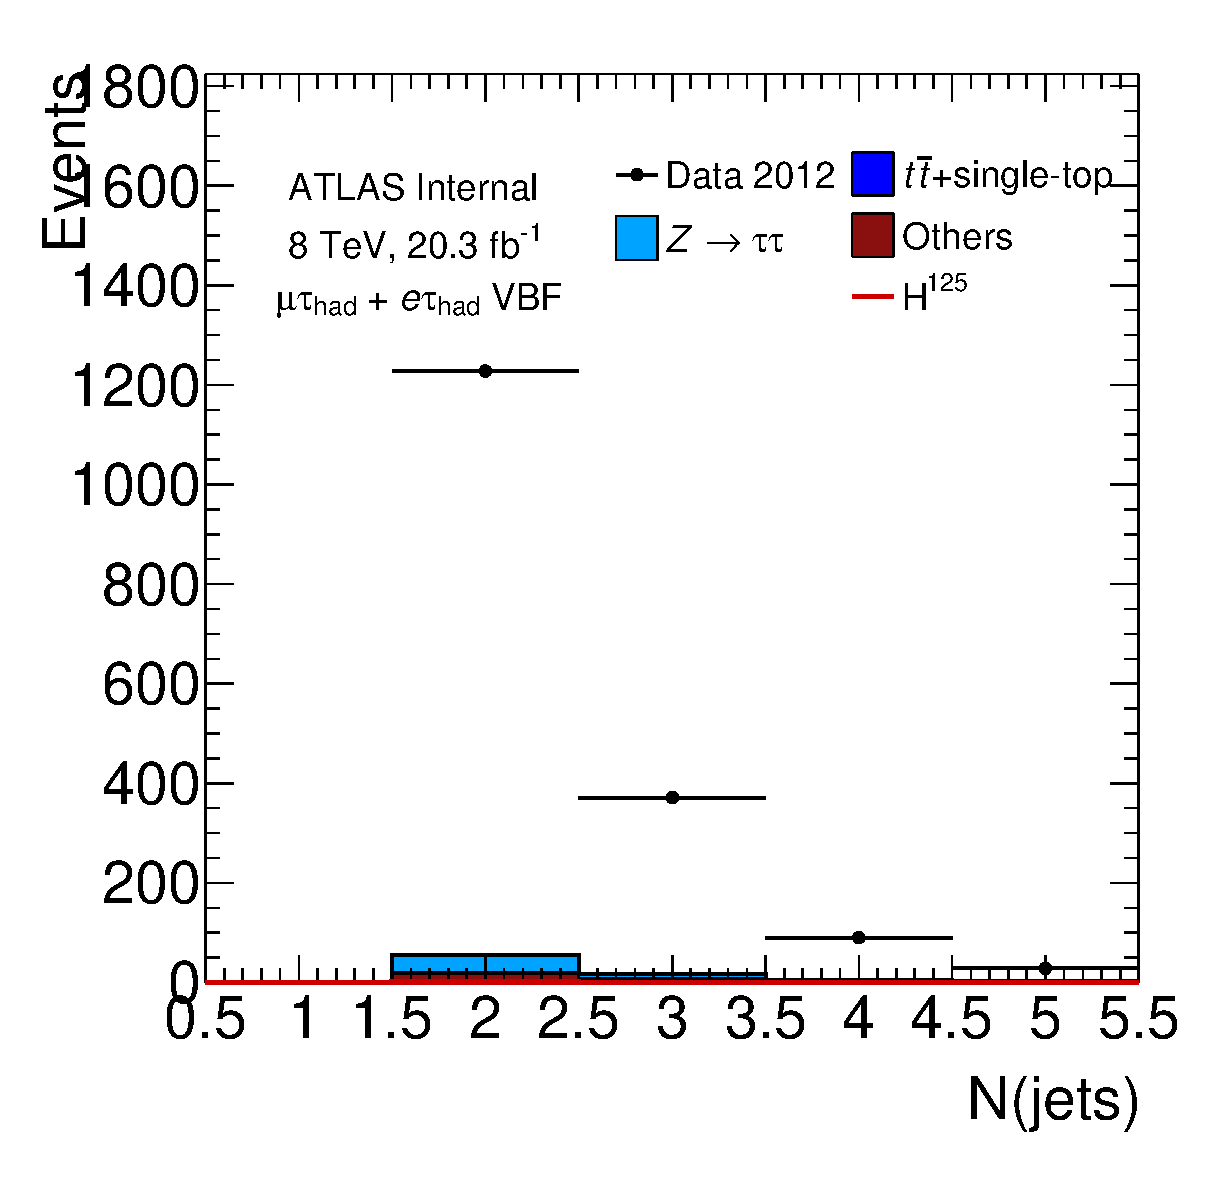
\includegraphics[width=0.32\textwidth]{figures/antitaus/n-jets30}
  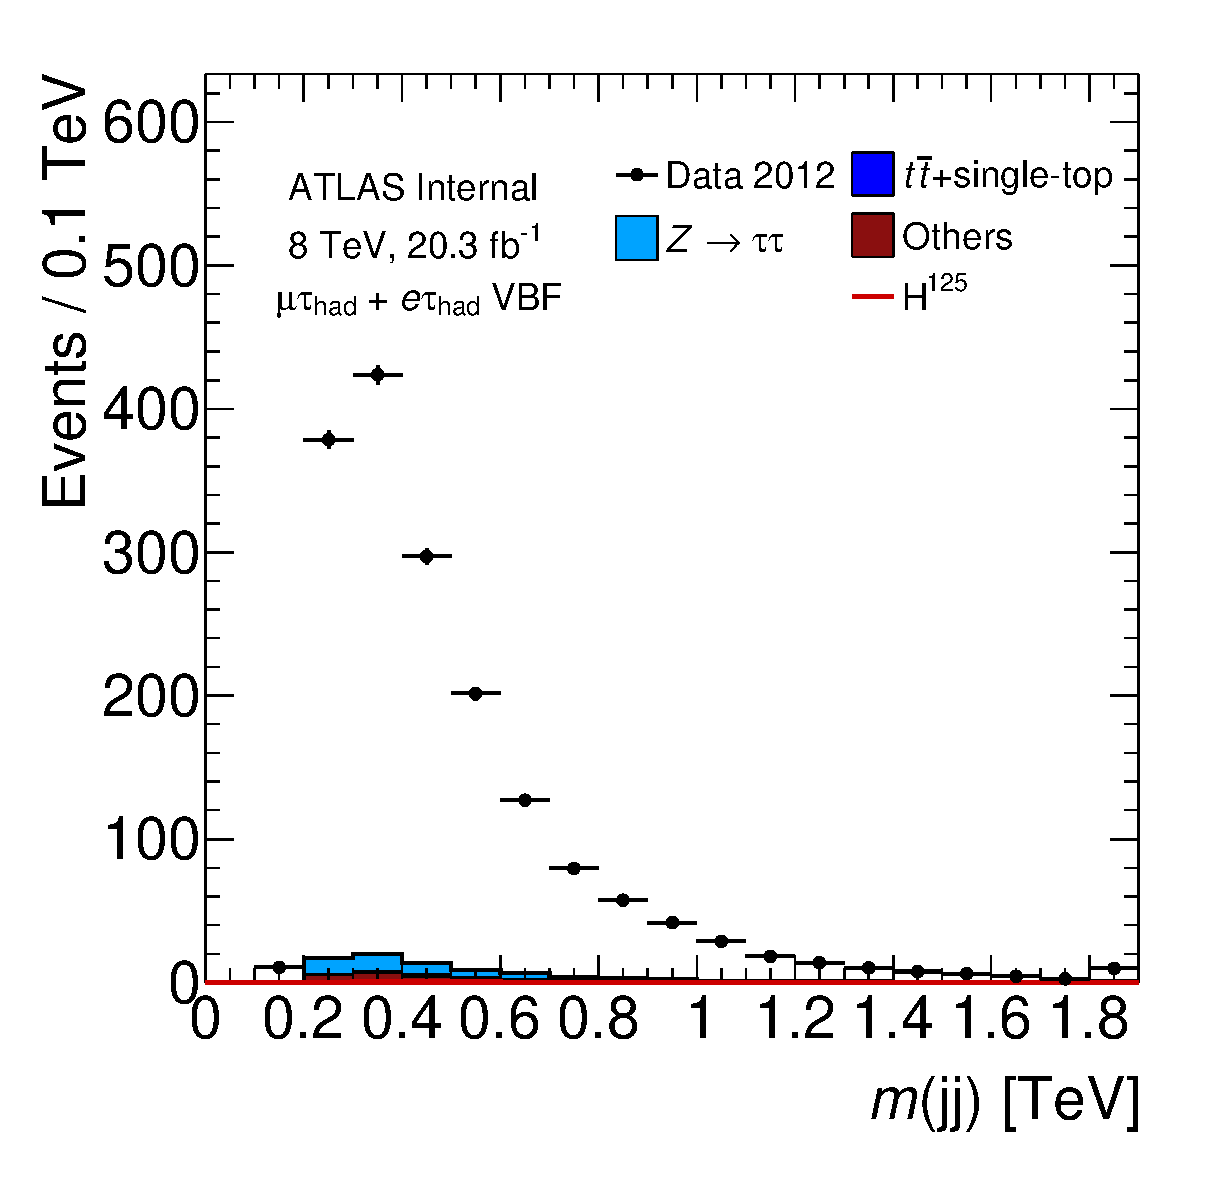
\includegraphics[width=0.32\textwidth]{figures/antitaus/dijet-m-veryhigh}
  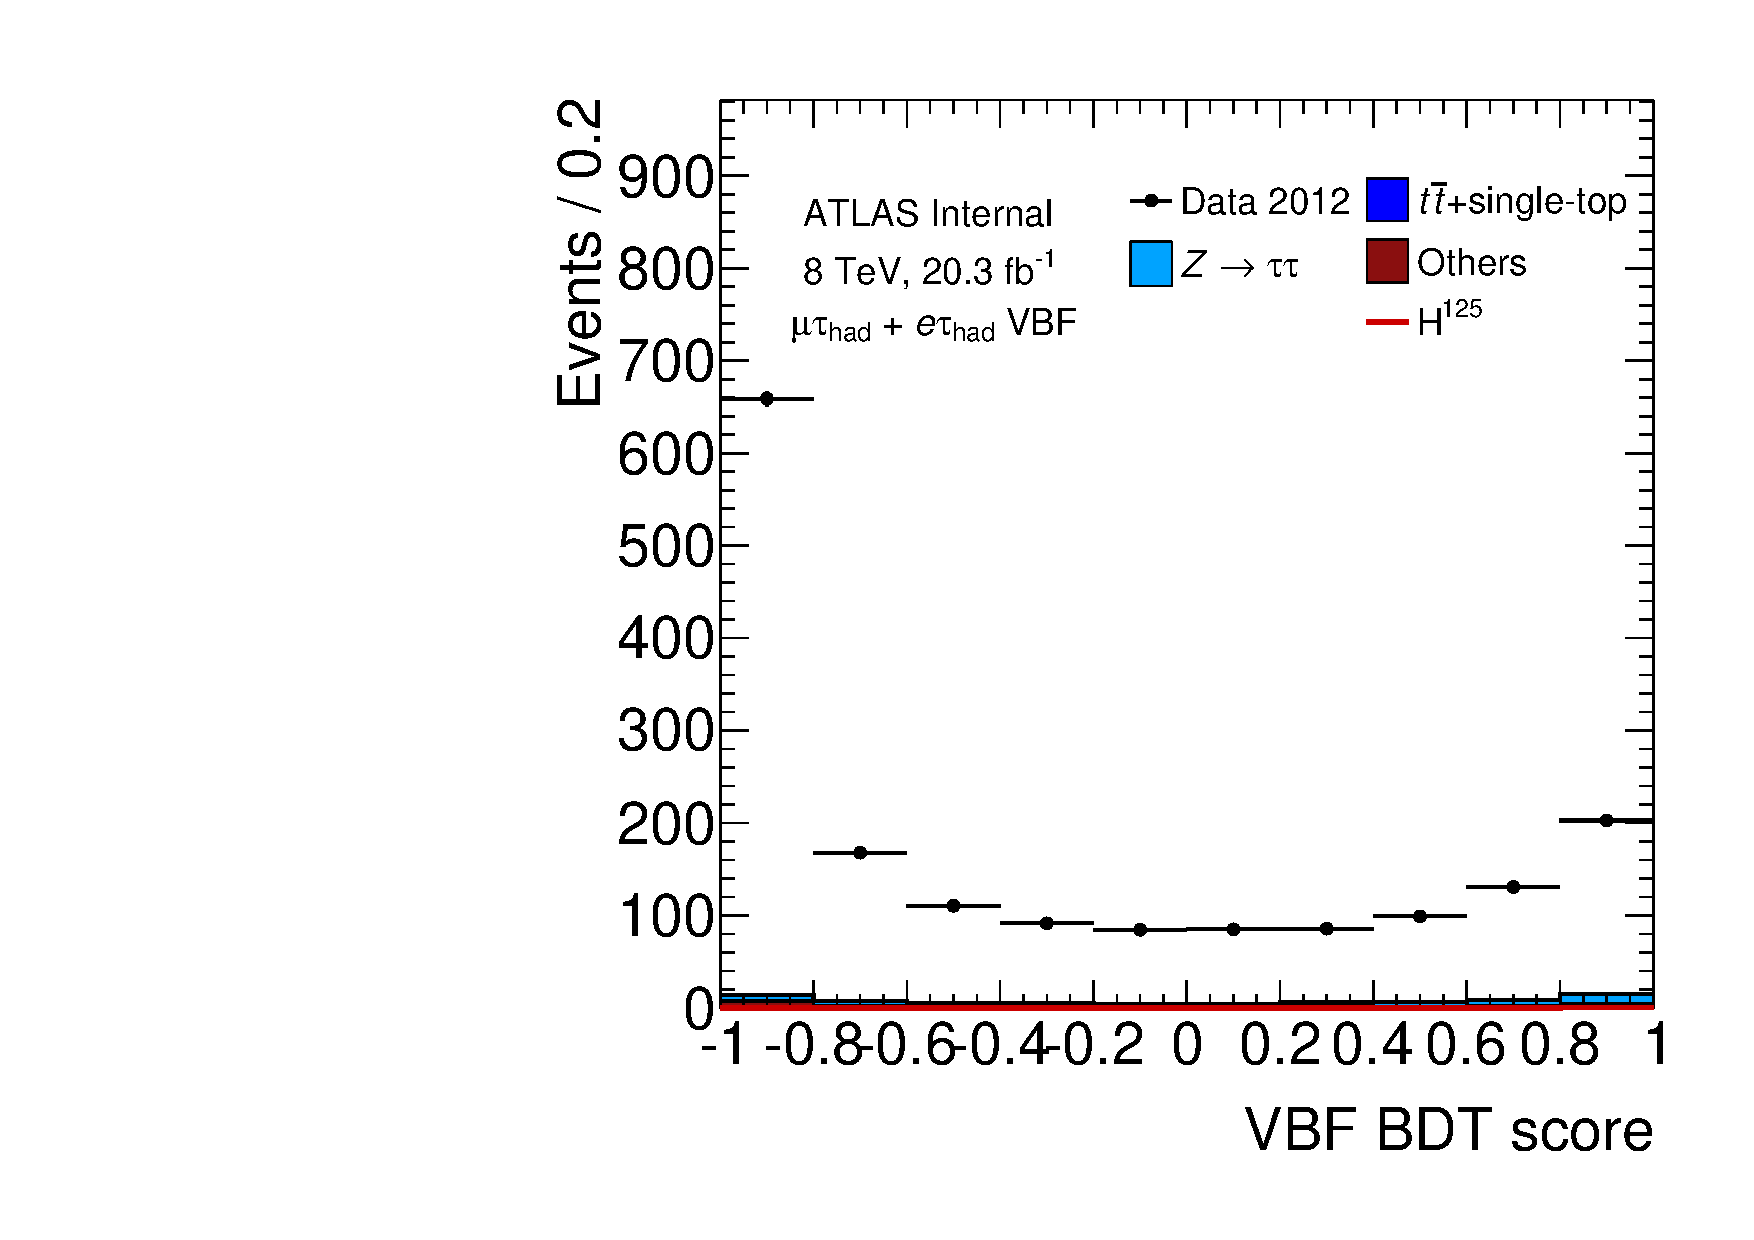
\includegraphics[width=0.32\textwidth]{figures/antitaus/BDTEve-VBF}
  \caption{Data events in the VBF category which fail $\tauh$ identification but fulfill all other requirements. The contamination of $\Ztautaulh$ and other processes without $\fakes$ is less than 10\%.}
  \label{fig:backgrounds-antitaus-jets}
\end{figure}

\clearpage

\begin{figure}[tp]
  \centering
  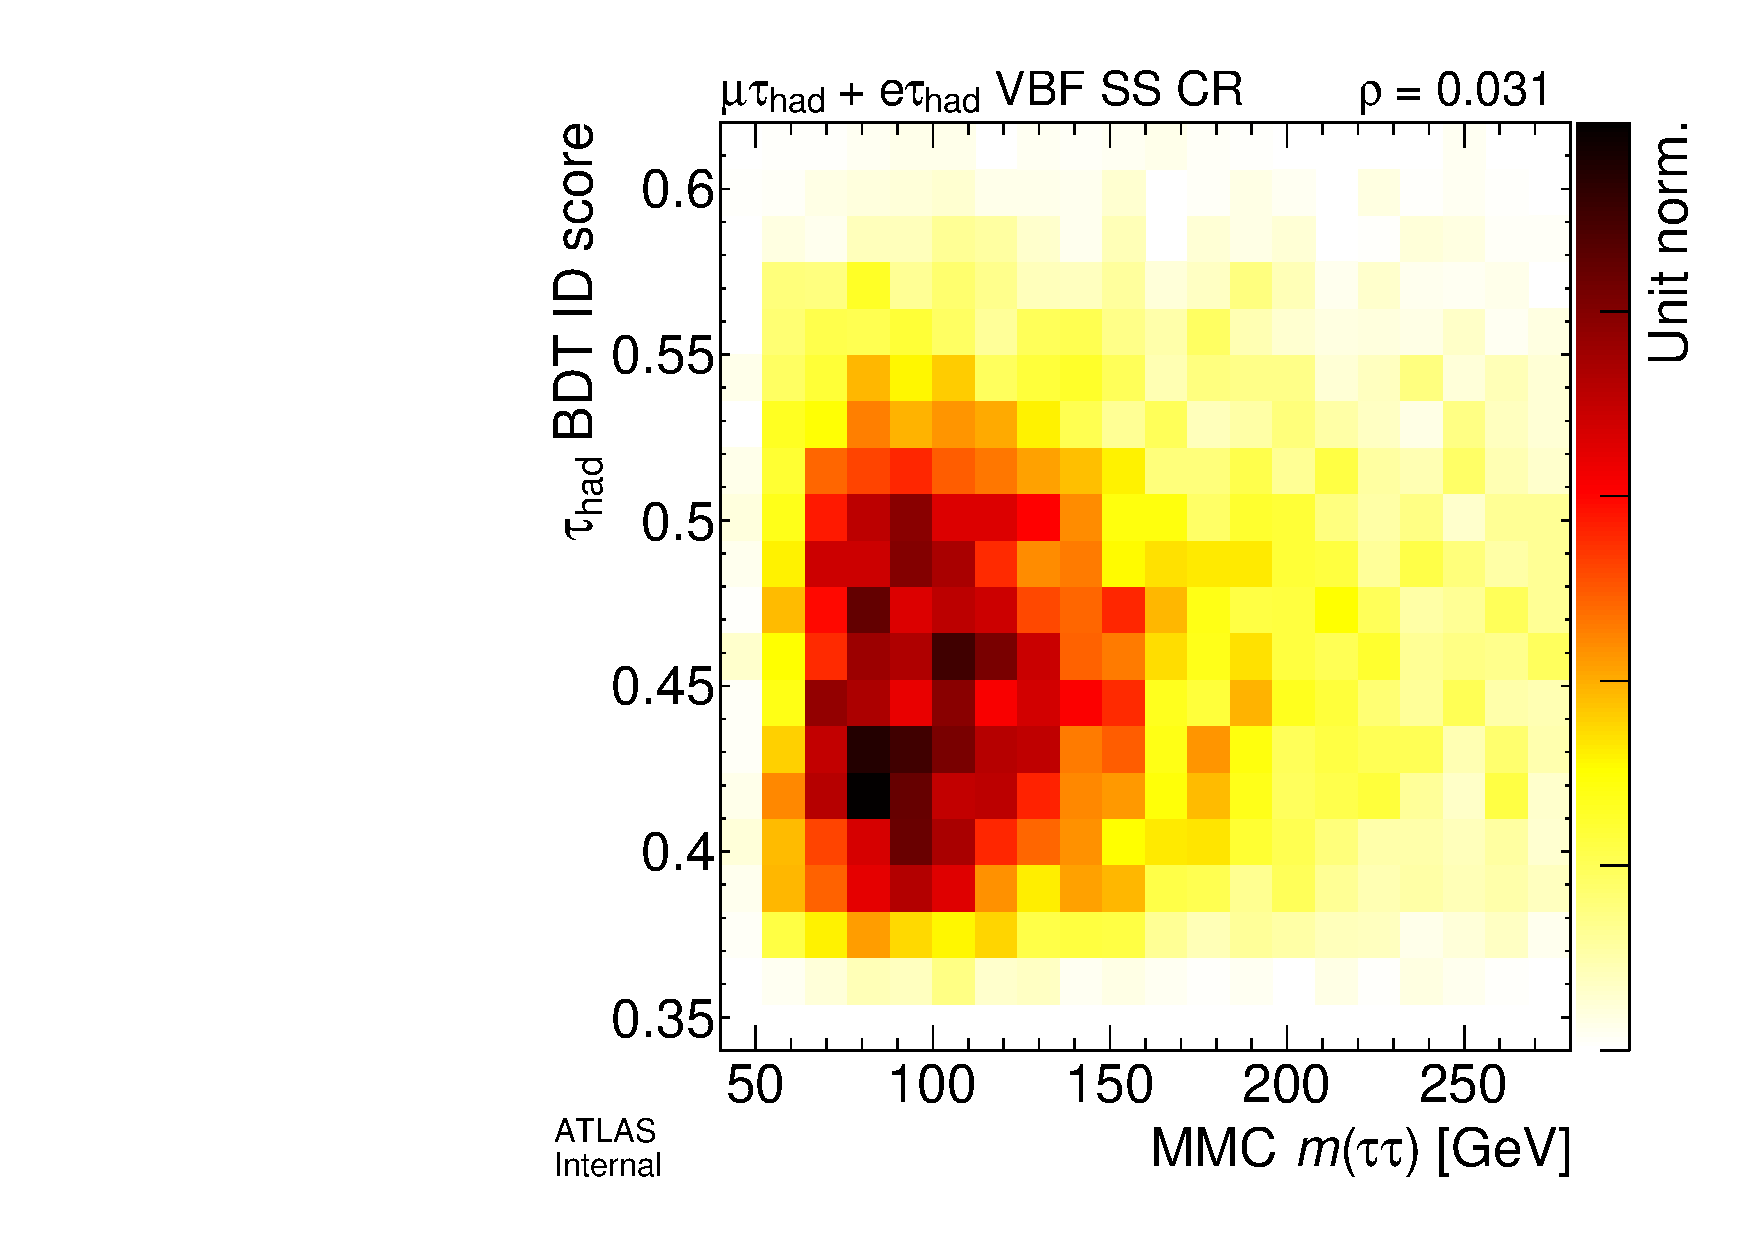
\includegraphics[width=0.32\textwidth]{figures/tauidcorrelations/tauid_vs_mMMC}
  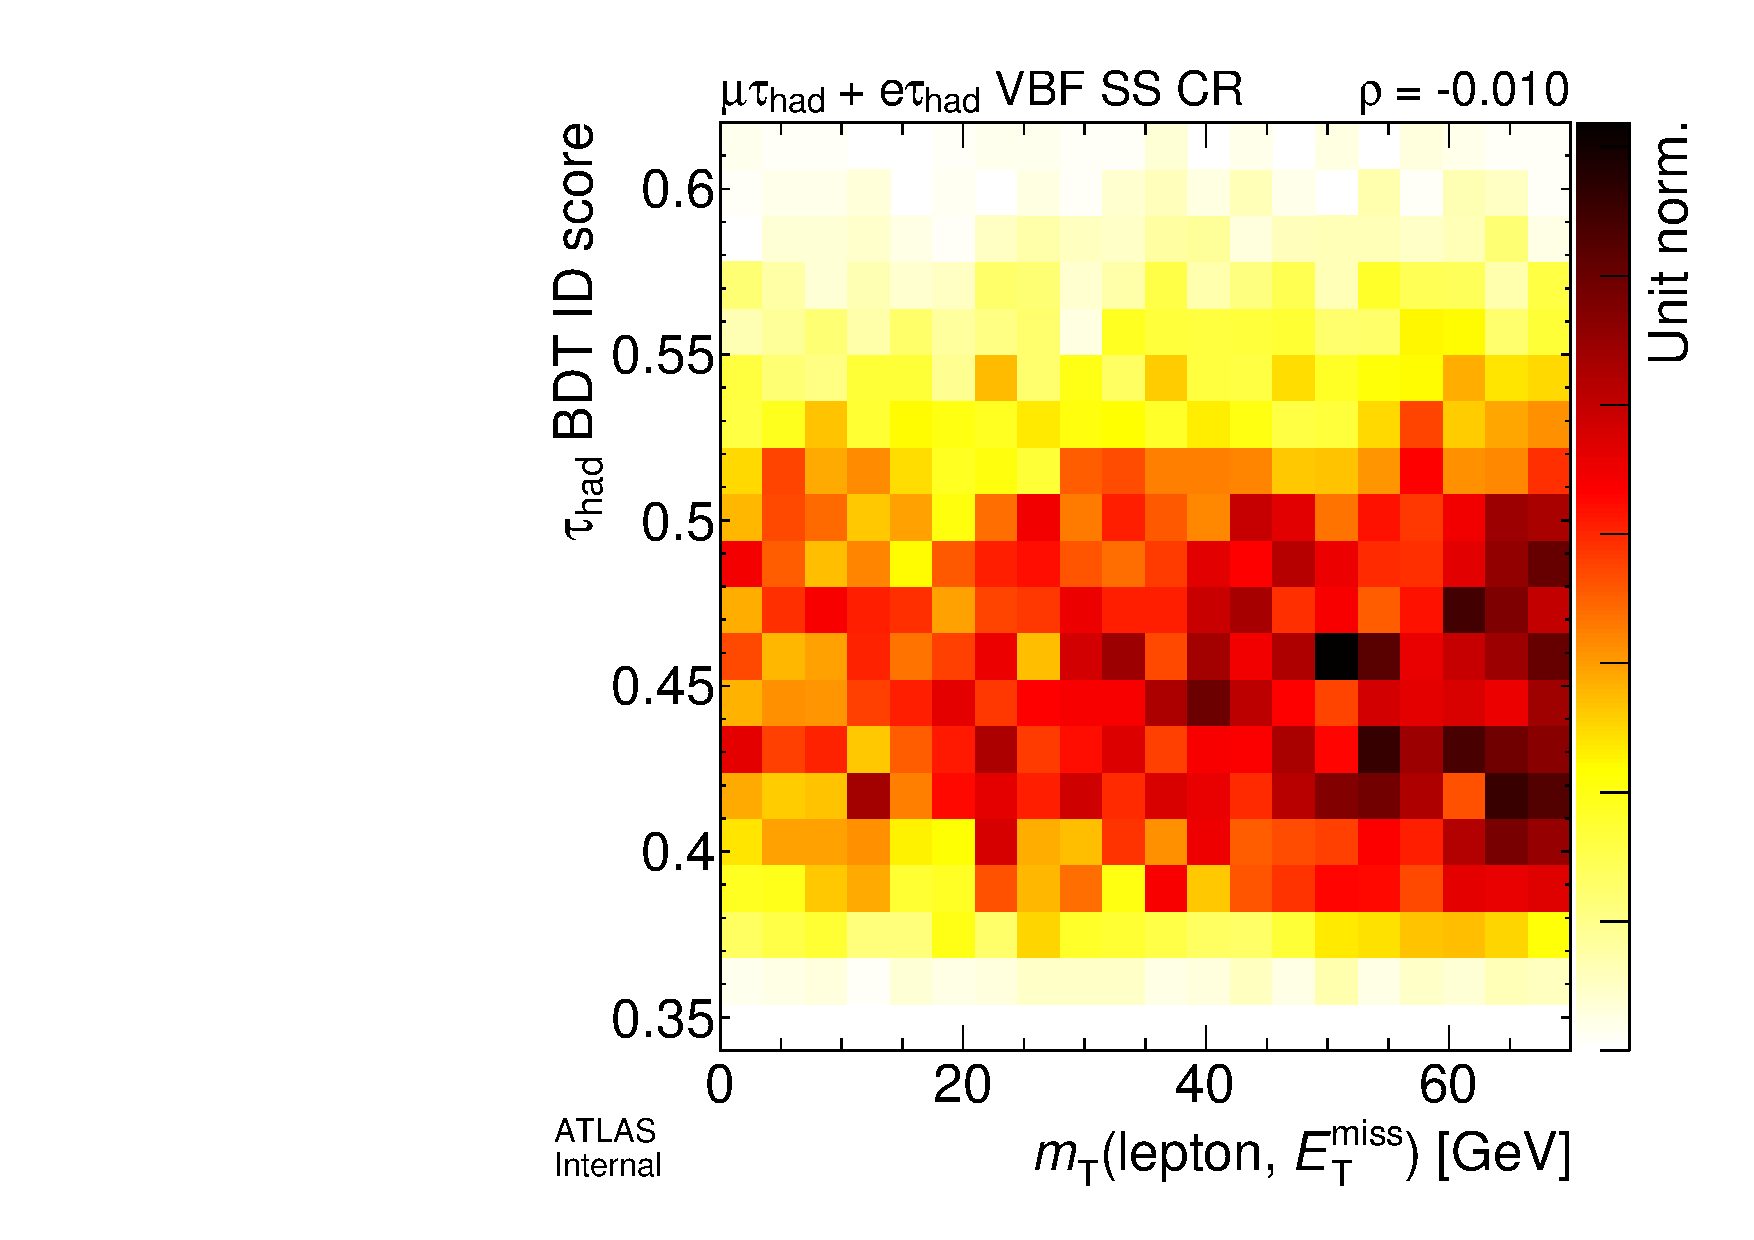
\includegraphics[width=0.32\textwidth]{figures/tauidcorrelations/tauid_vs_mT}
  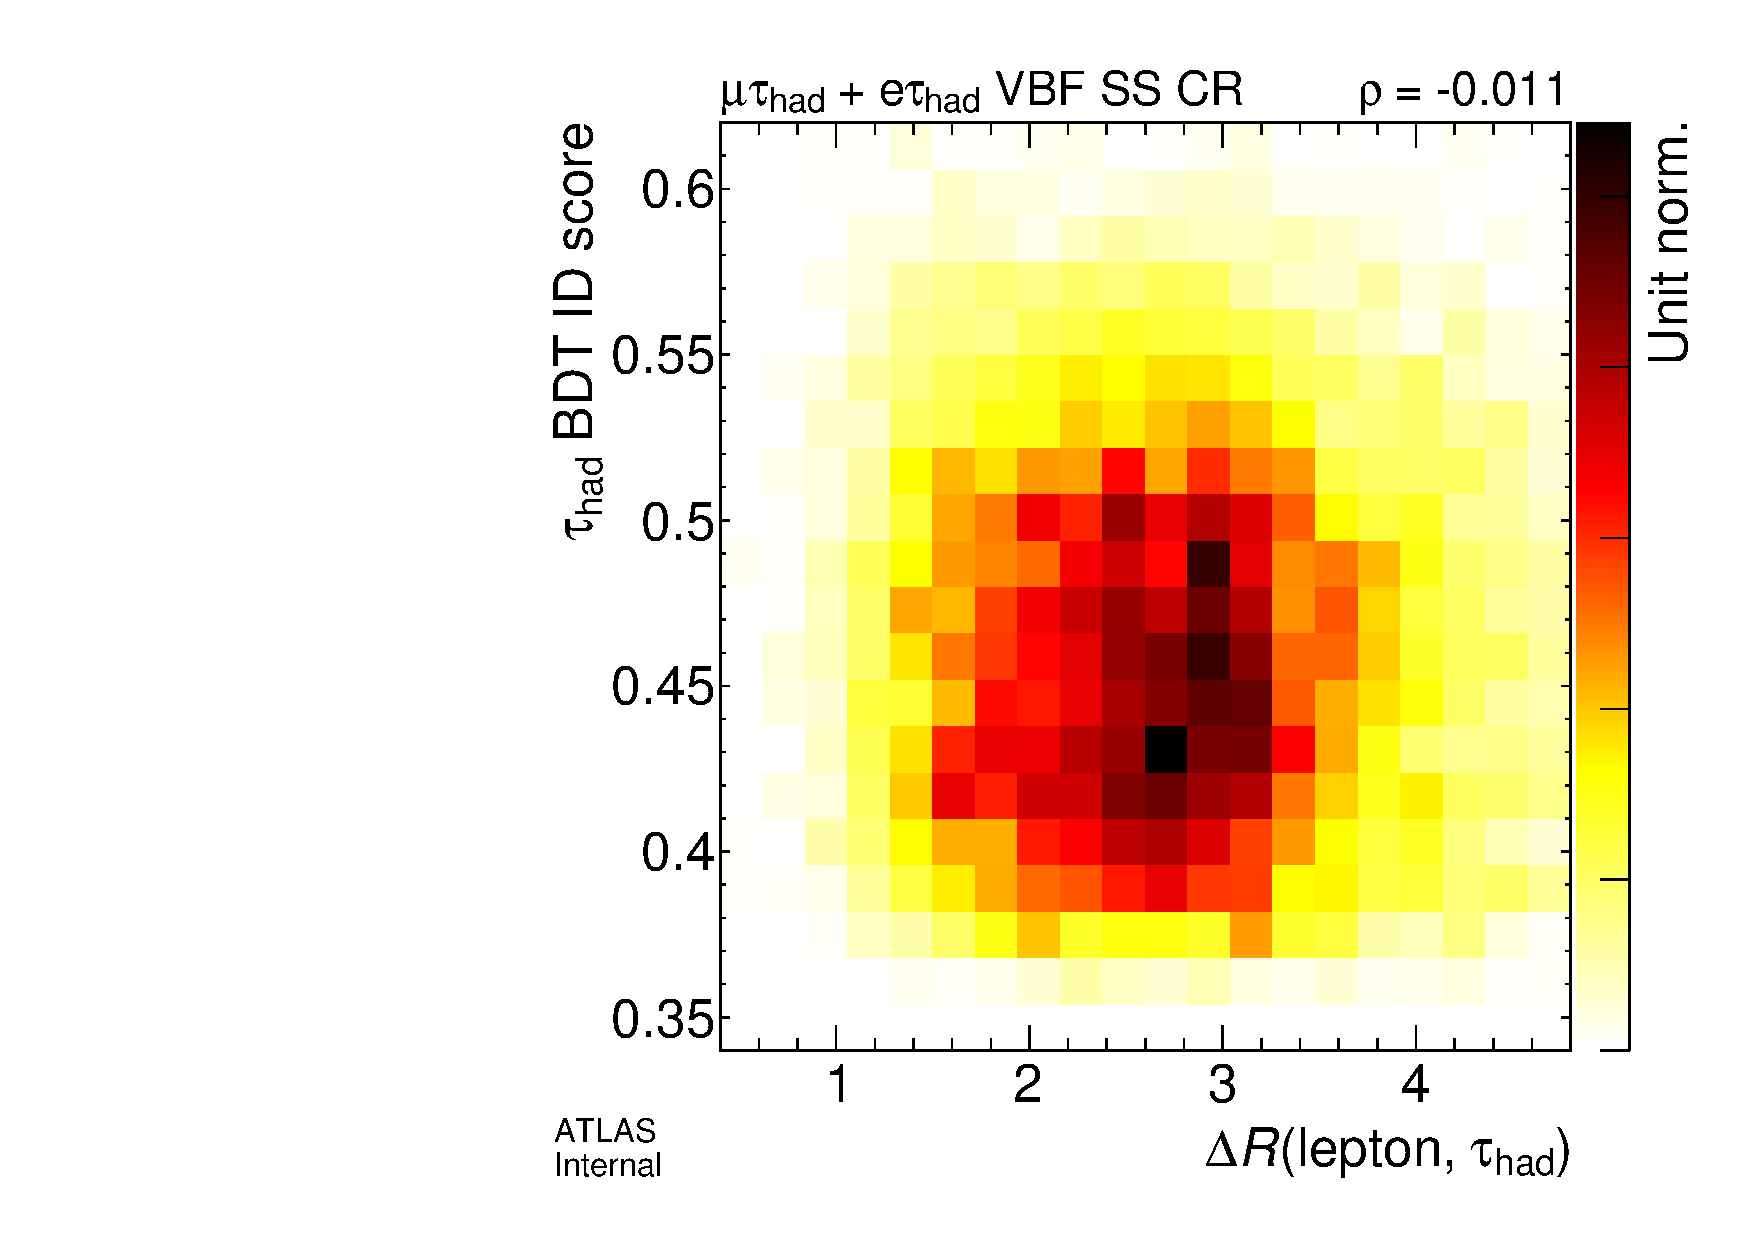
\includegraphics[width=0.32\textwidth]{figures/tauidcorrelations/tauid_vs_dR}
  % --------------
  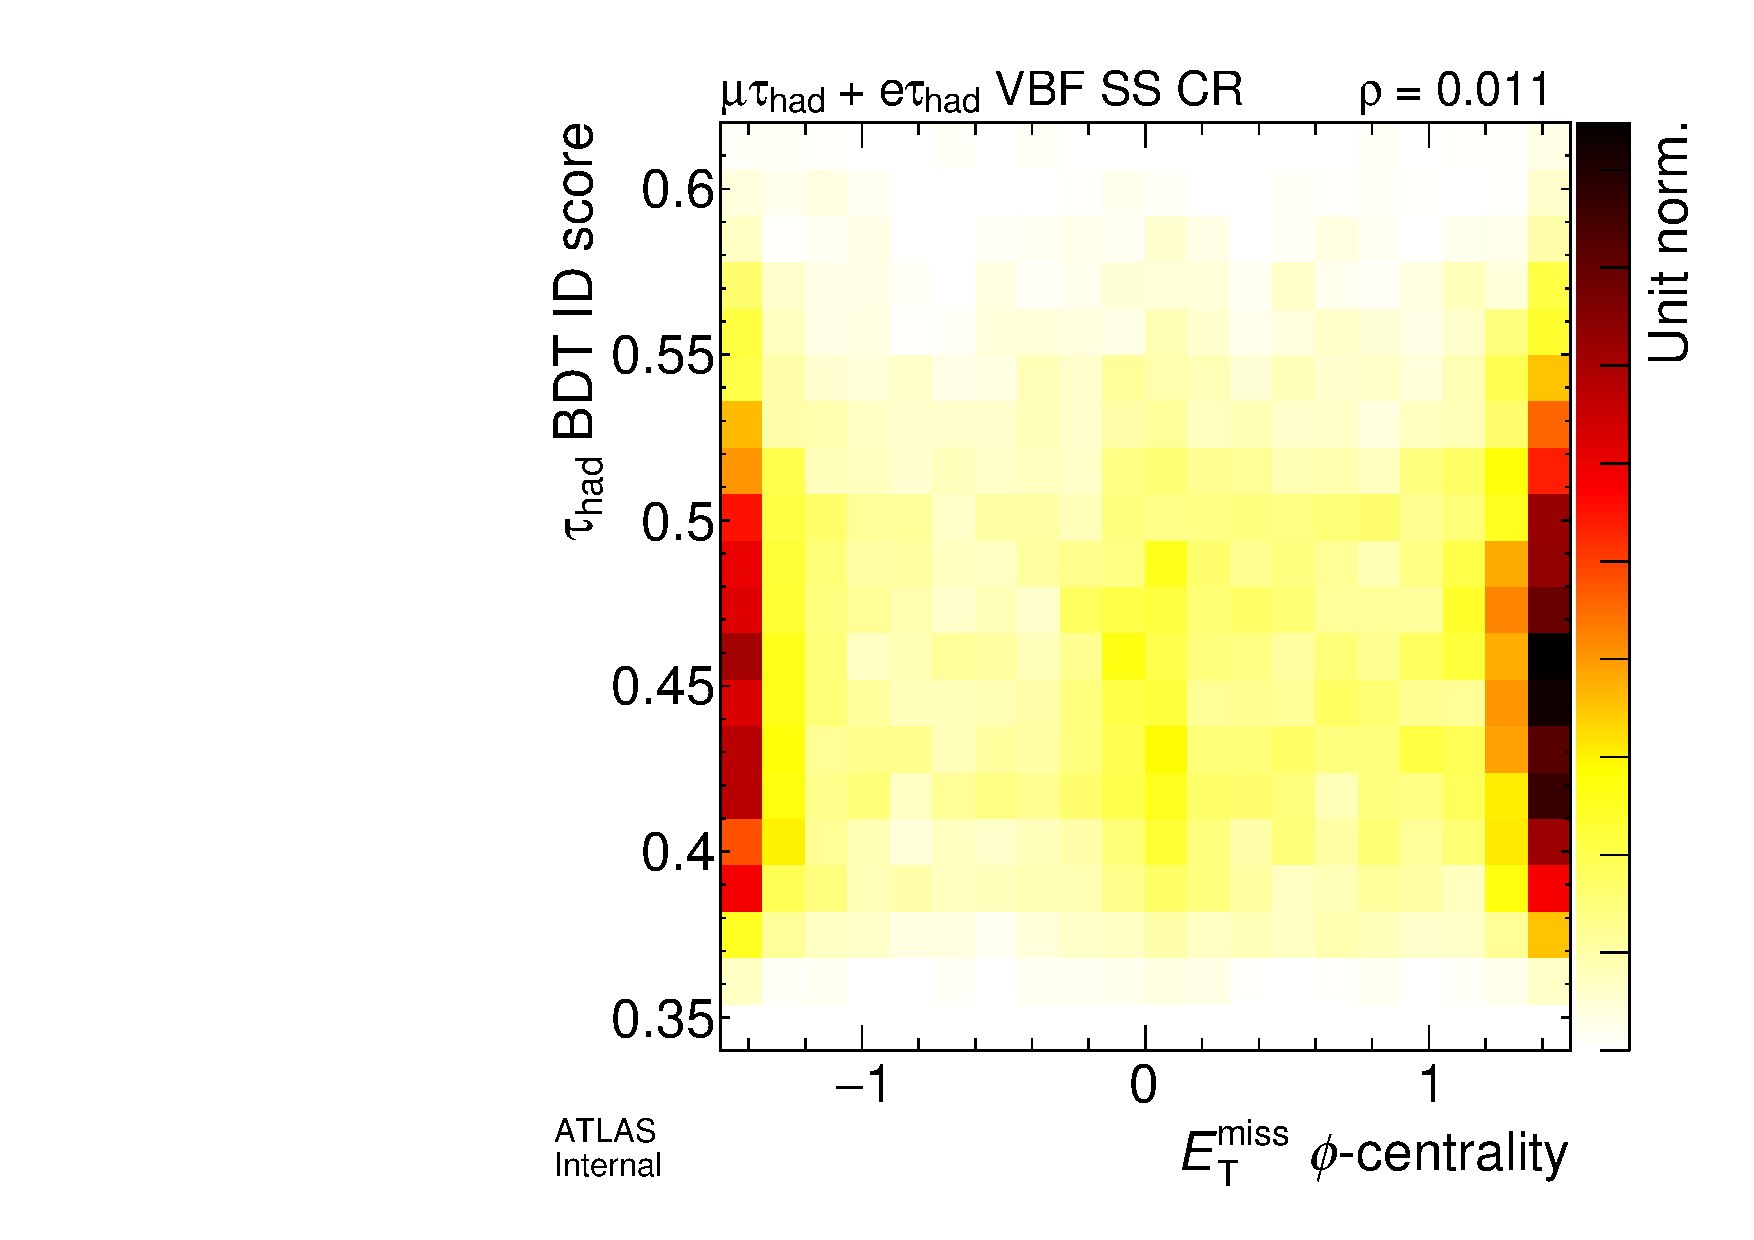
\includegraphics[width=0.32\textwidth]{figures/tauidcorrelations/tauid_vs_metphi}
  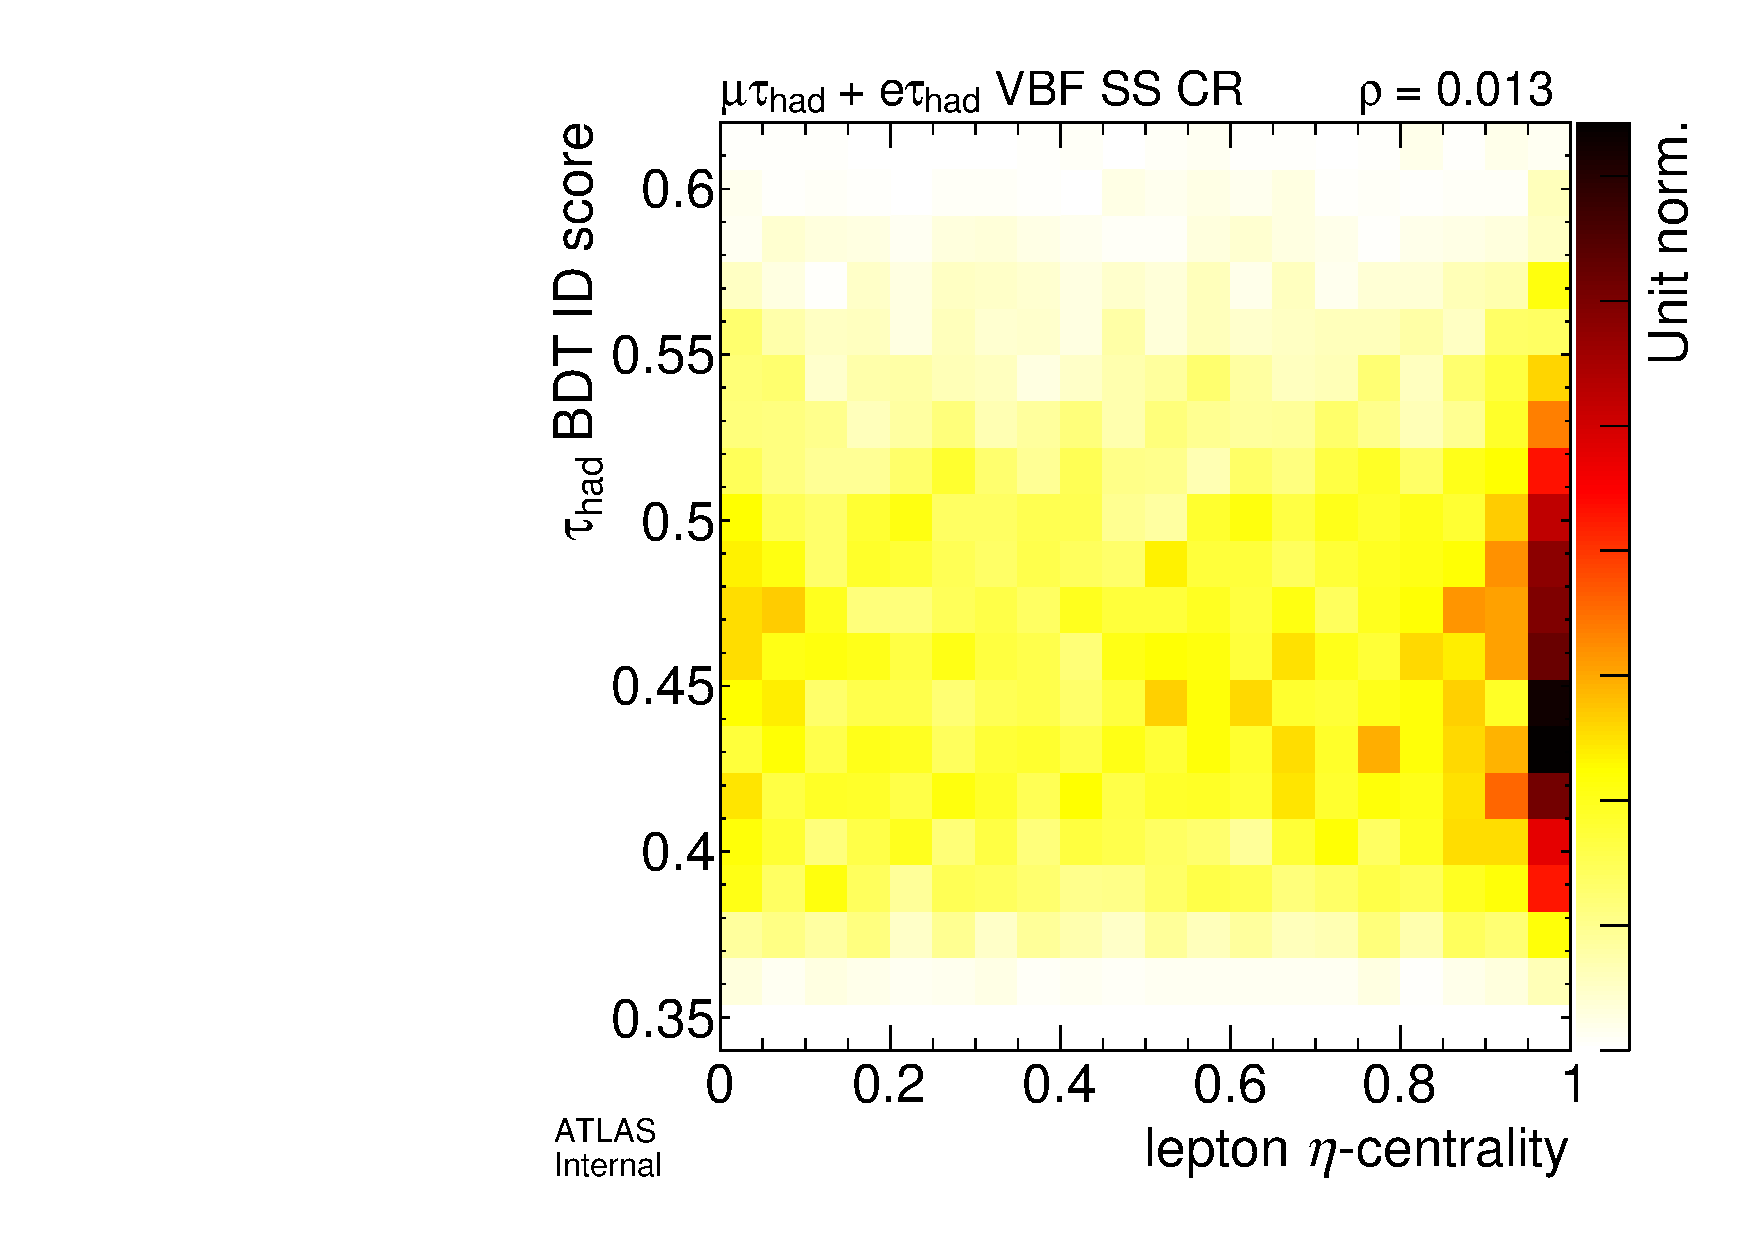
\includegraphics[width=0.32\textwidth]{figures/tauidcorrelations/tauid_vs_lepeta}
  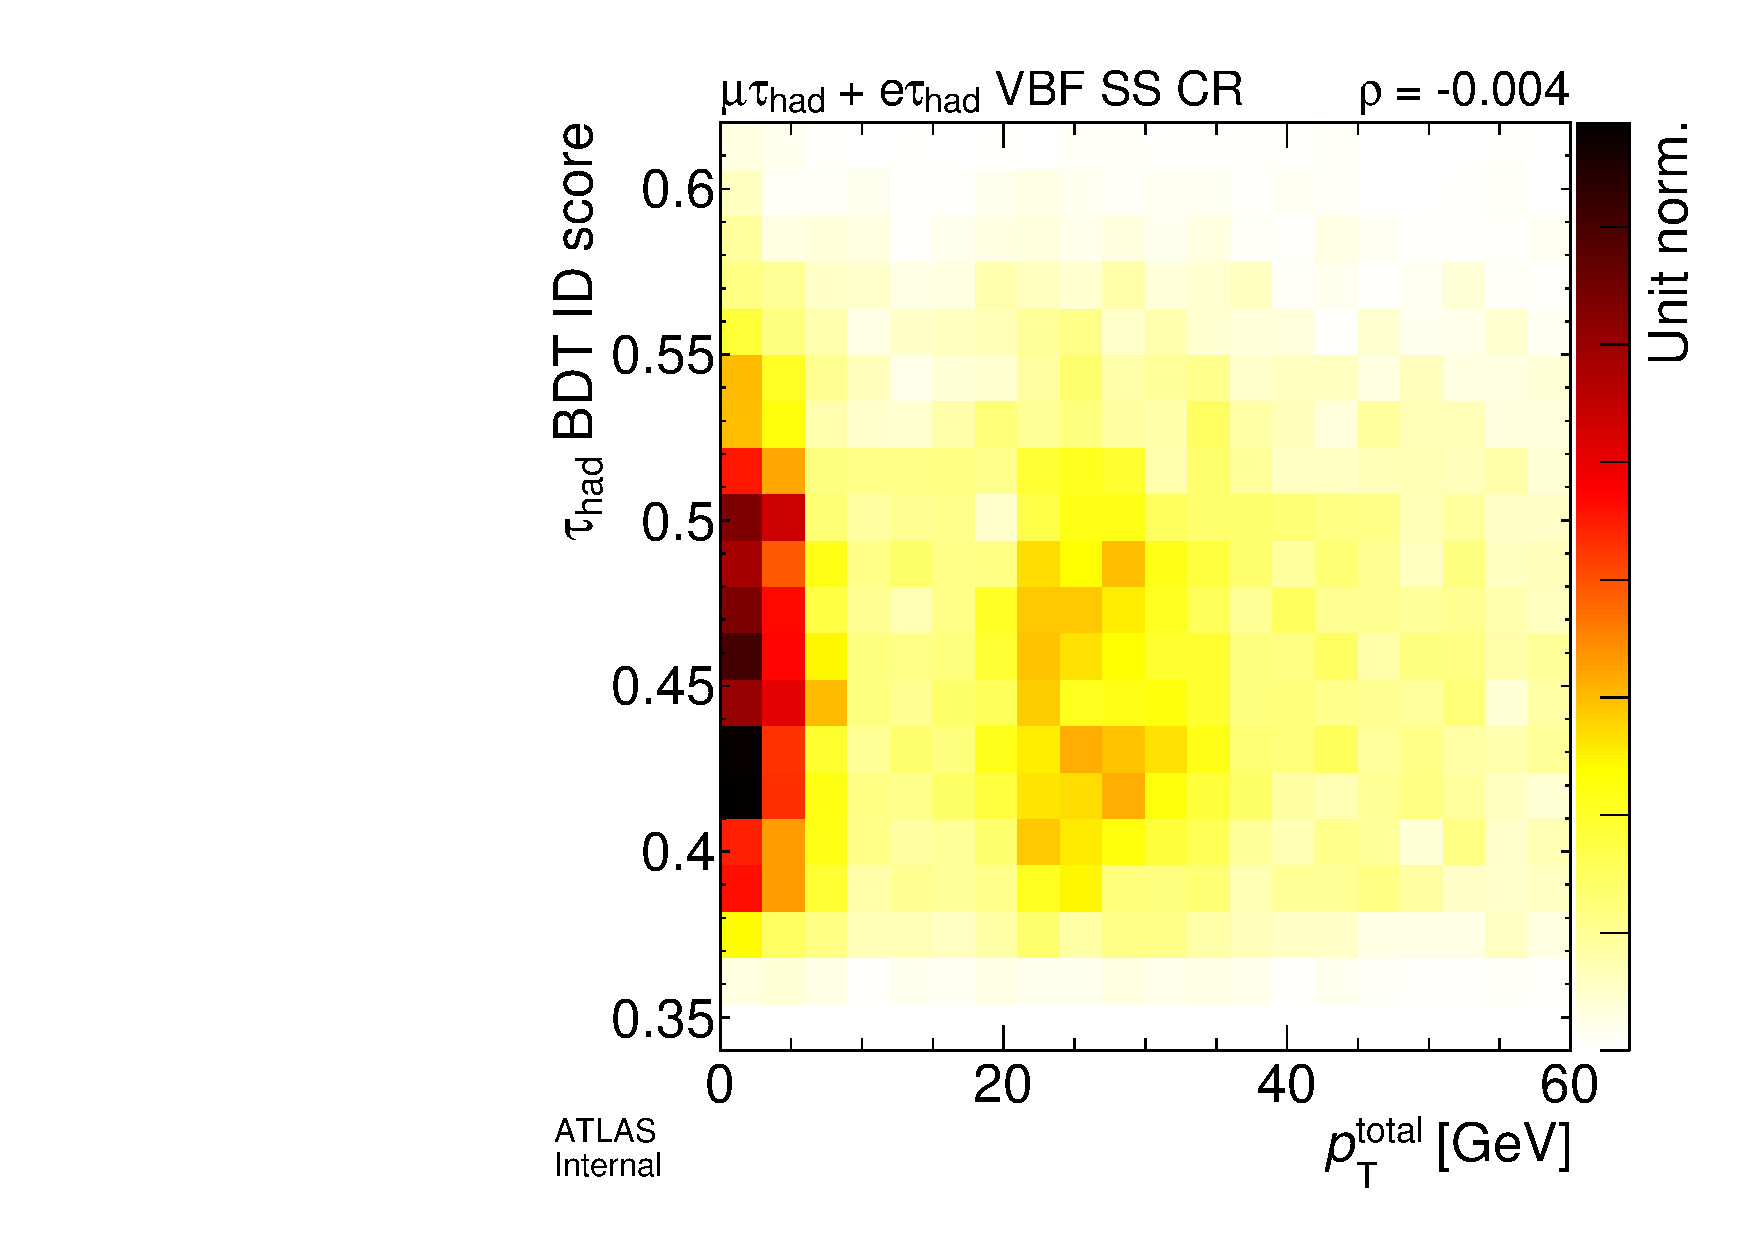
\includegraphics[width=0.32\textwidth]{figures/tauidcorrelations/tauid_vs_pttot}
  % --------------
  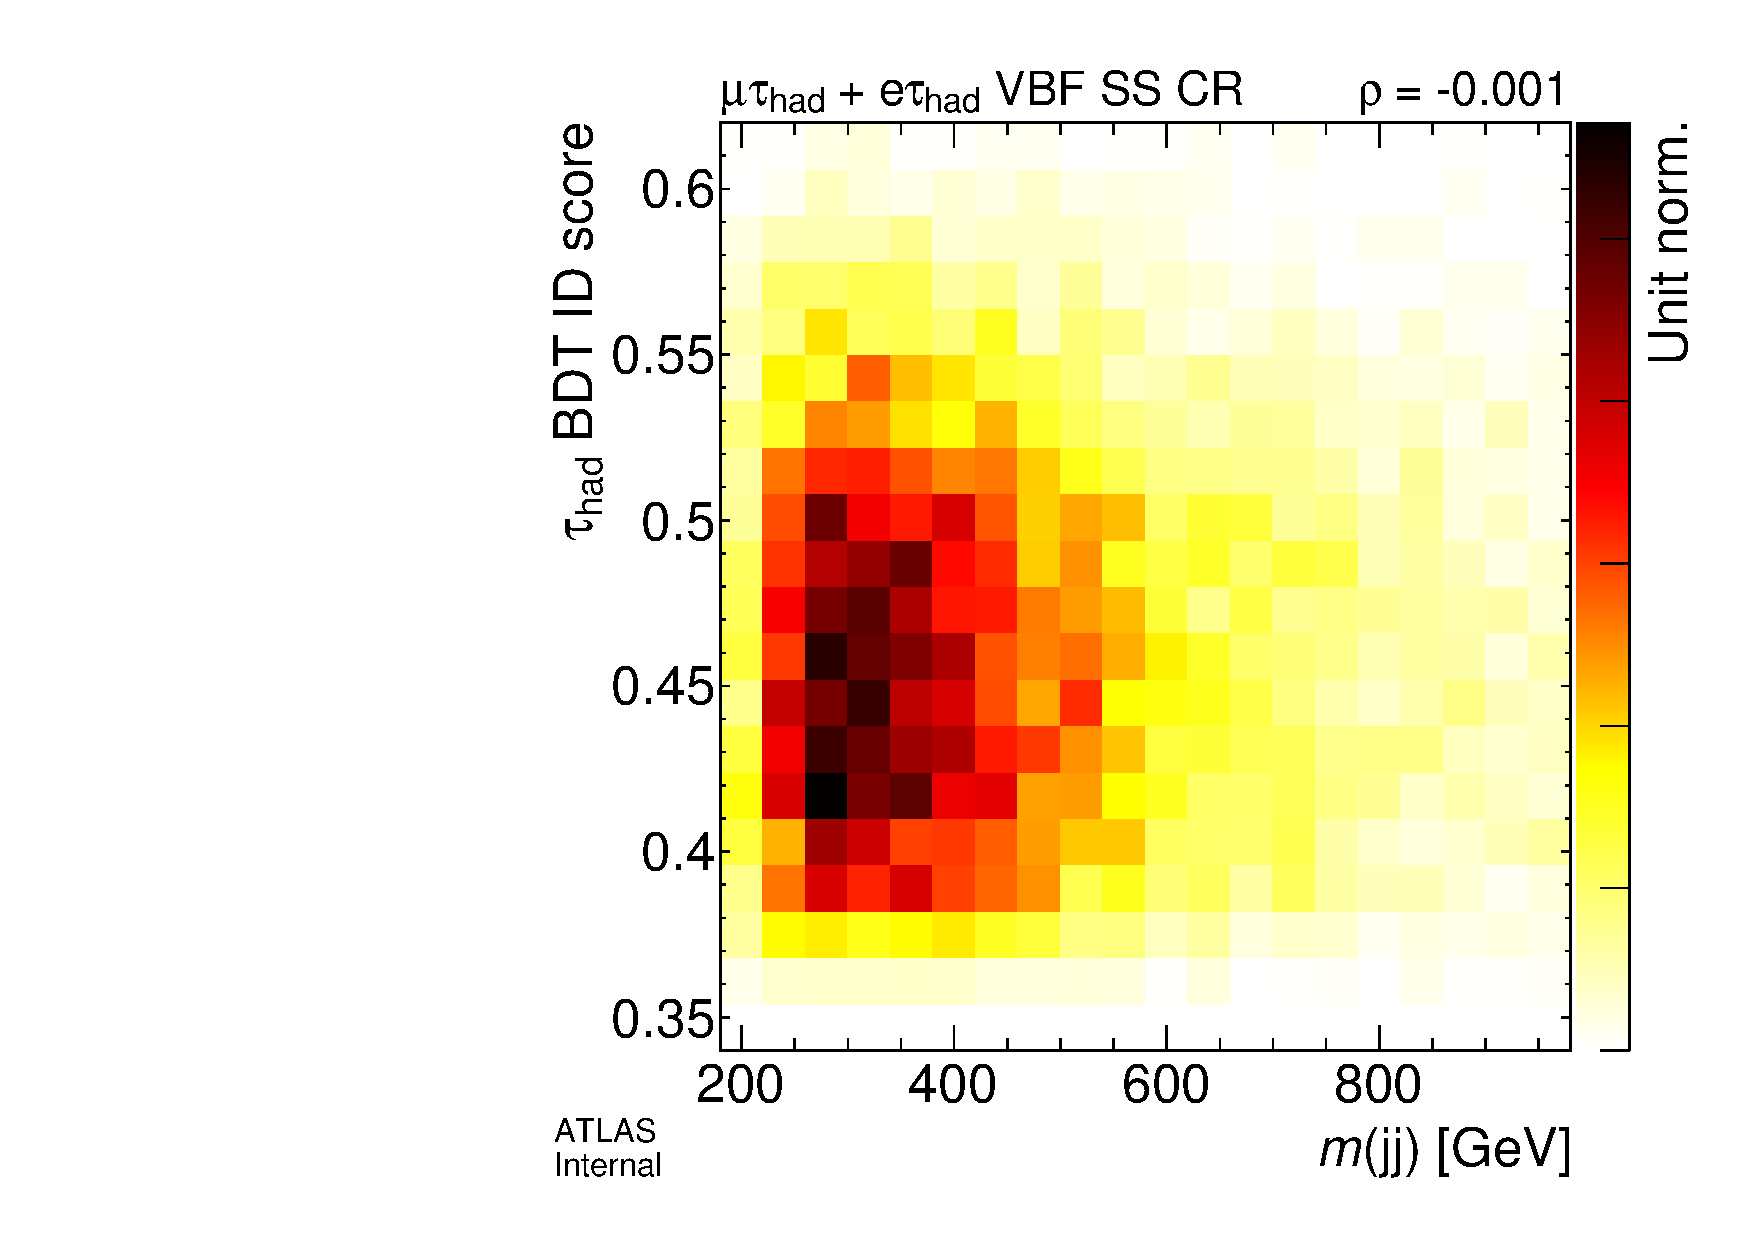
\includegraphics[width=0.32\textwidth]{figures/tauidcorrelations/tauid_vs_mjj}
  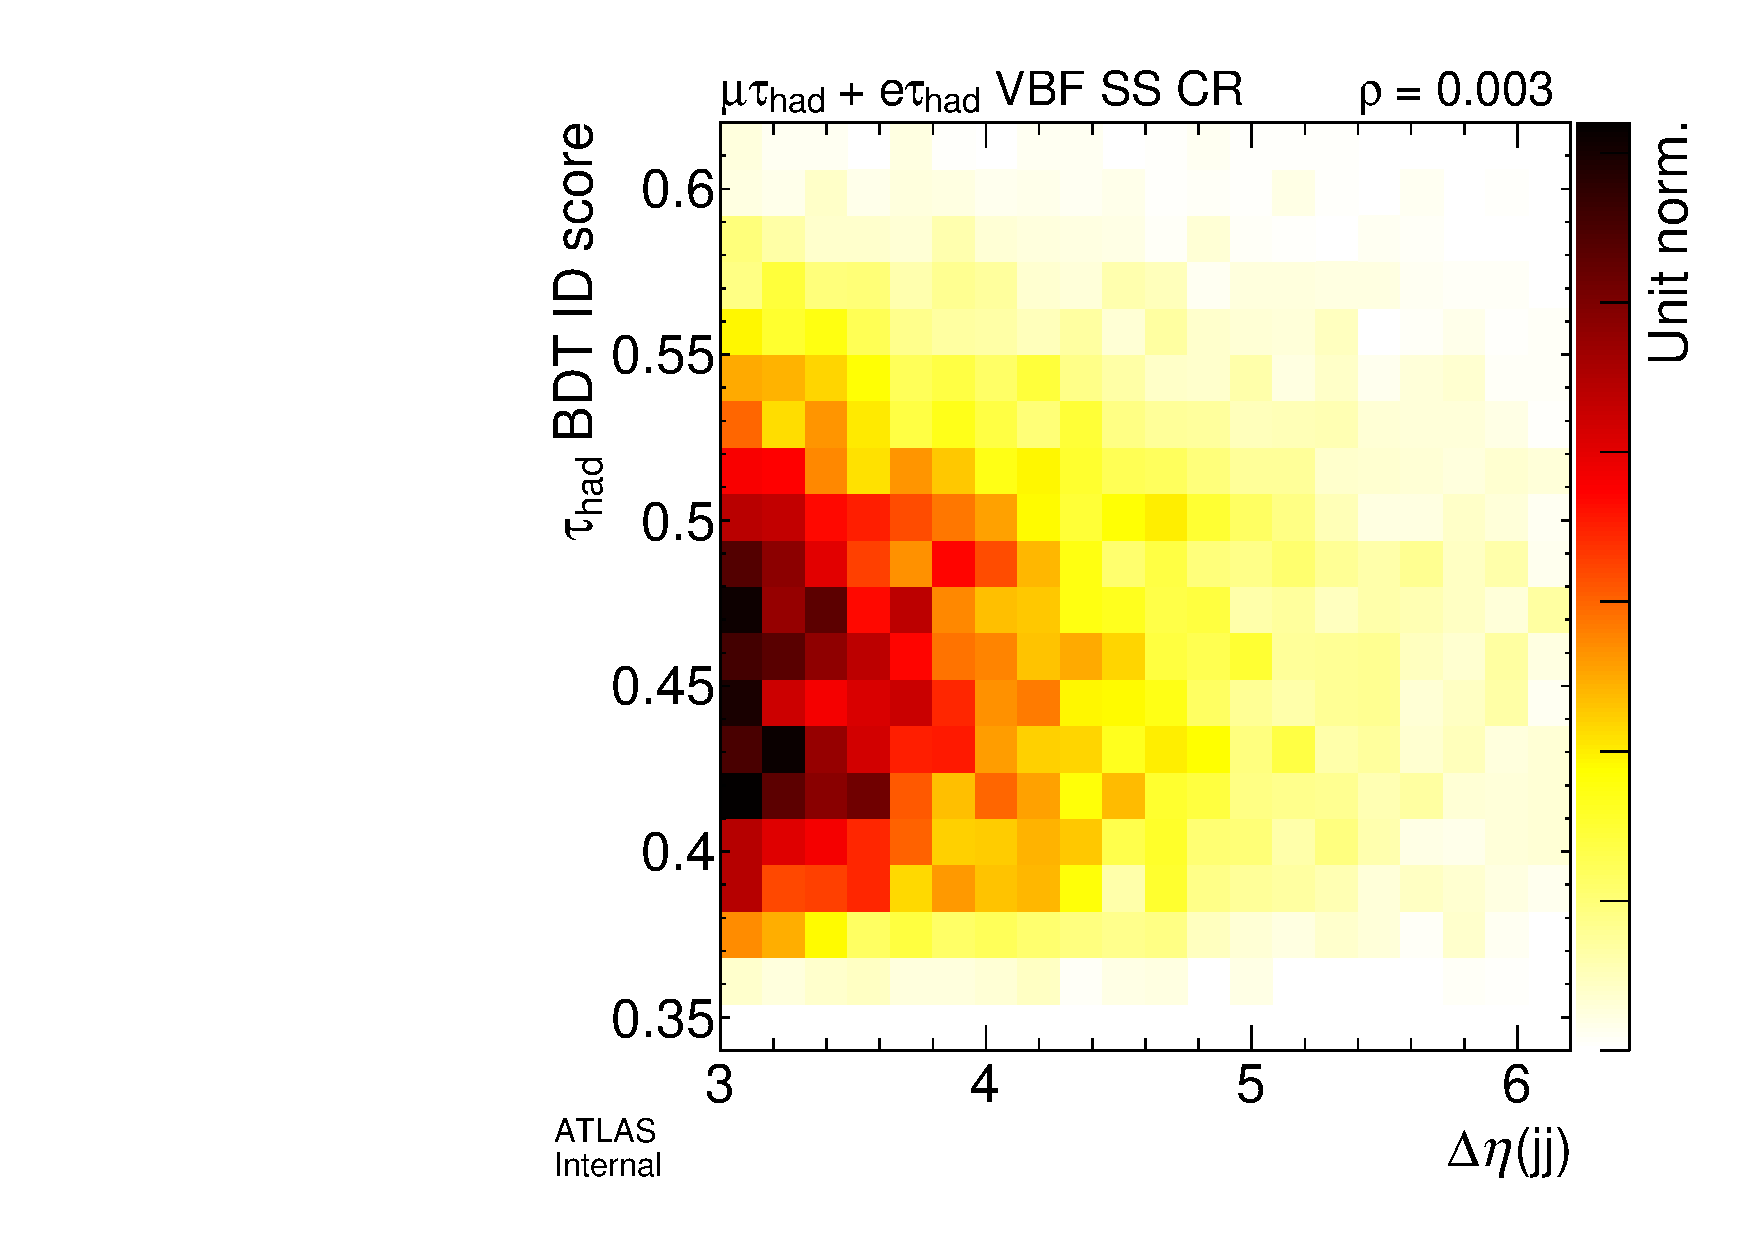
\includegraphics[width=0.32\textwidth]{figures/tauidcorrelations/tauid_vs_detajj}
  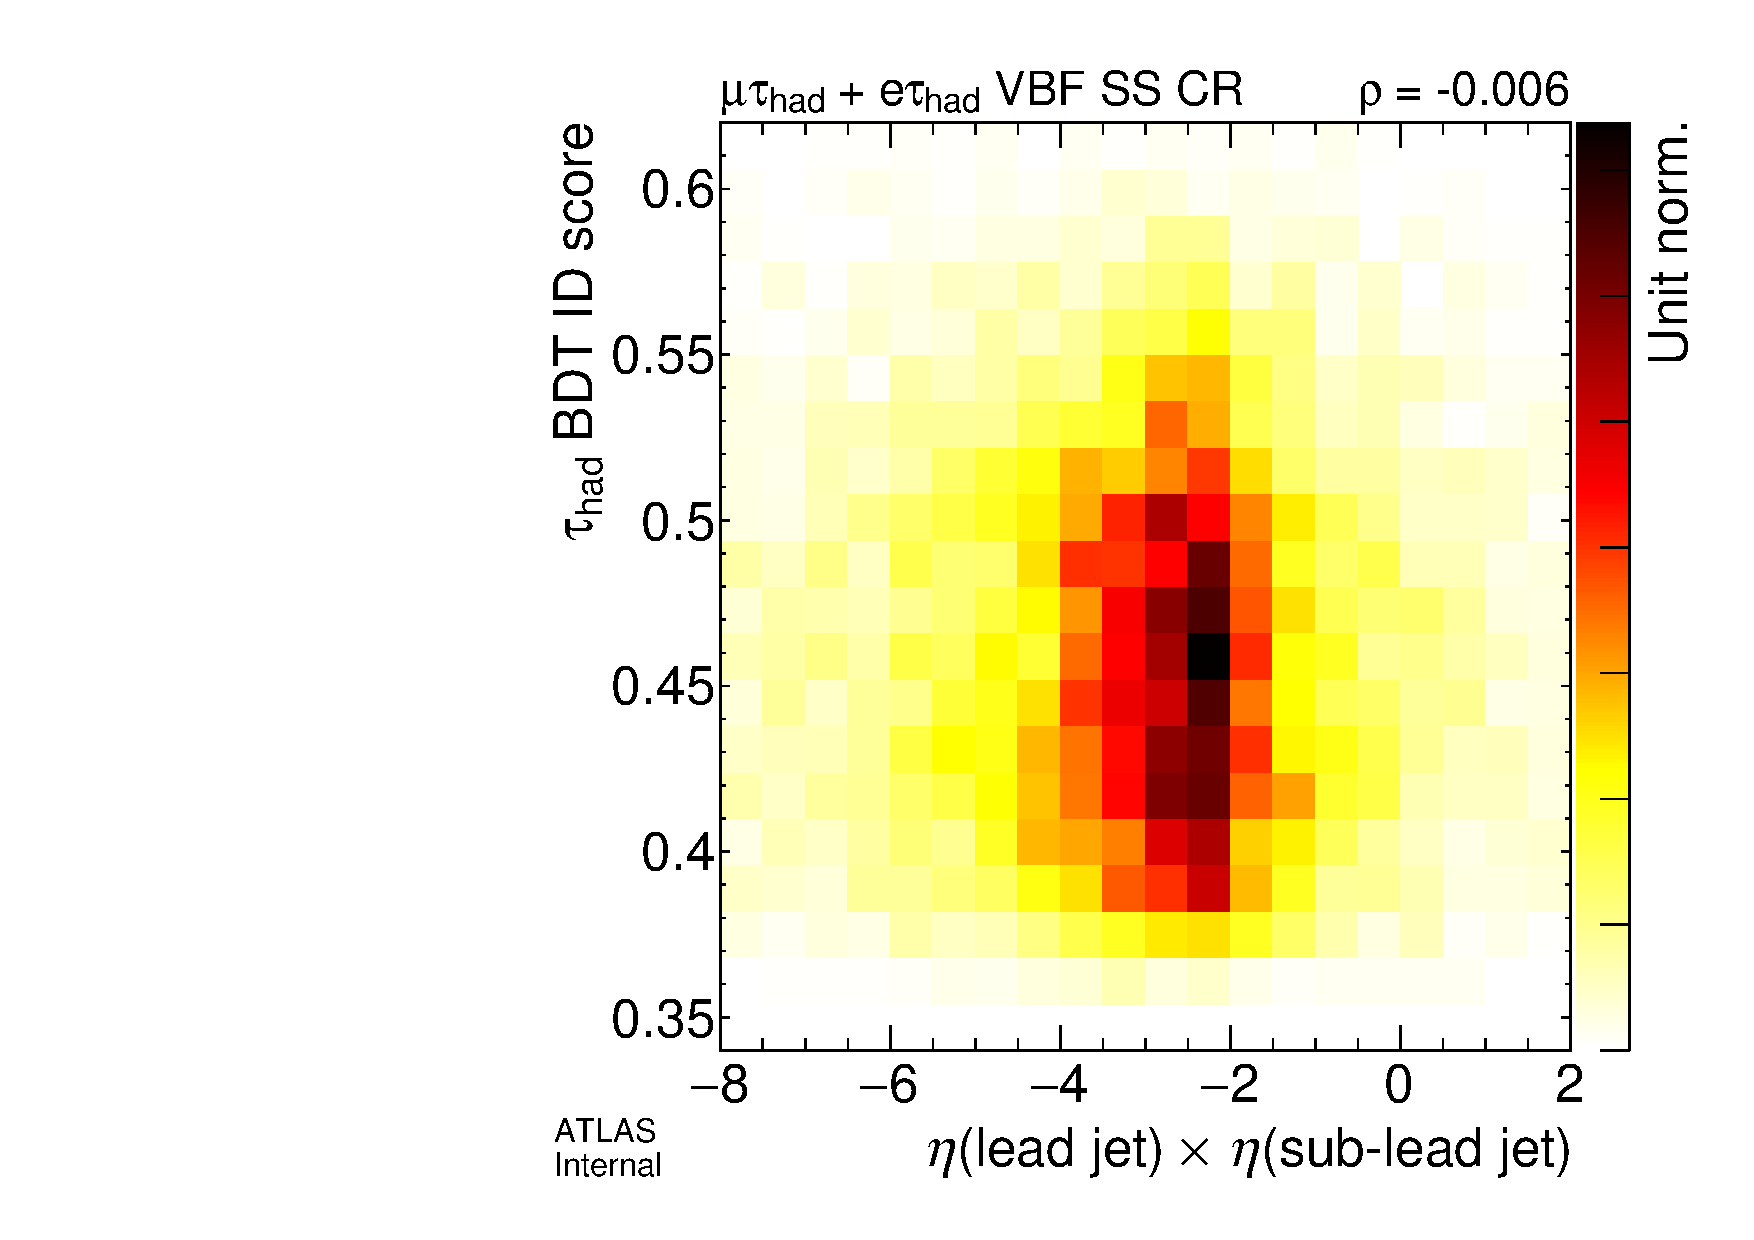
\includegraphics[width=0.32\textwidth]{figures/tauidcorrelations/tauid_vs_etaprod}
  % --------------
  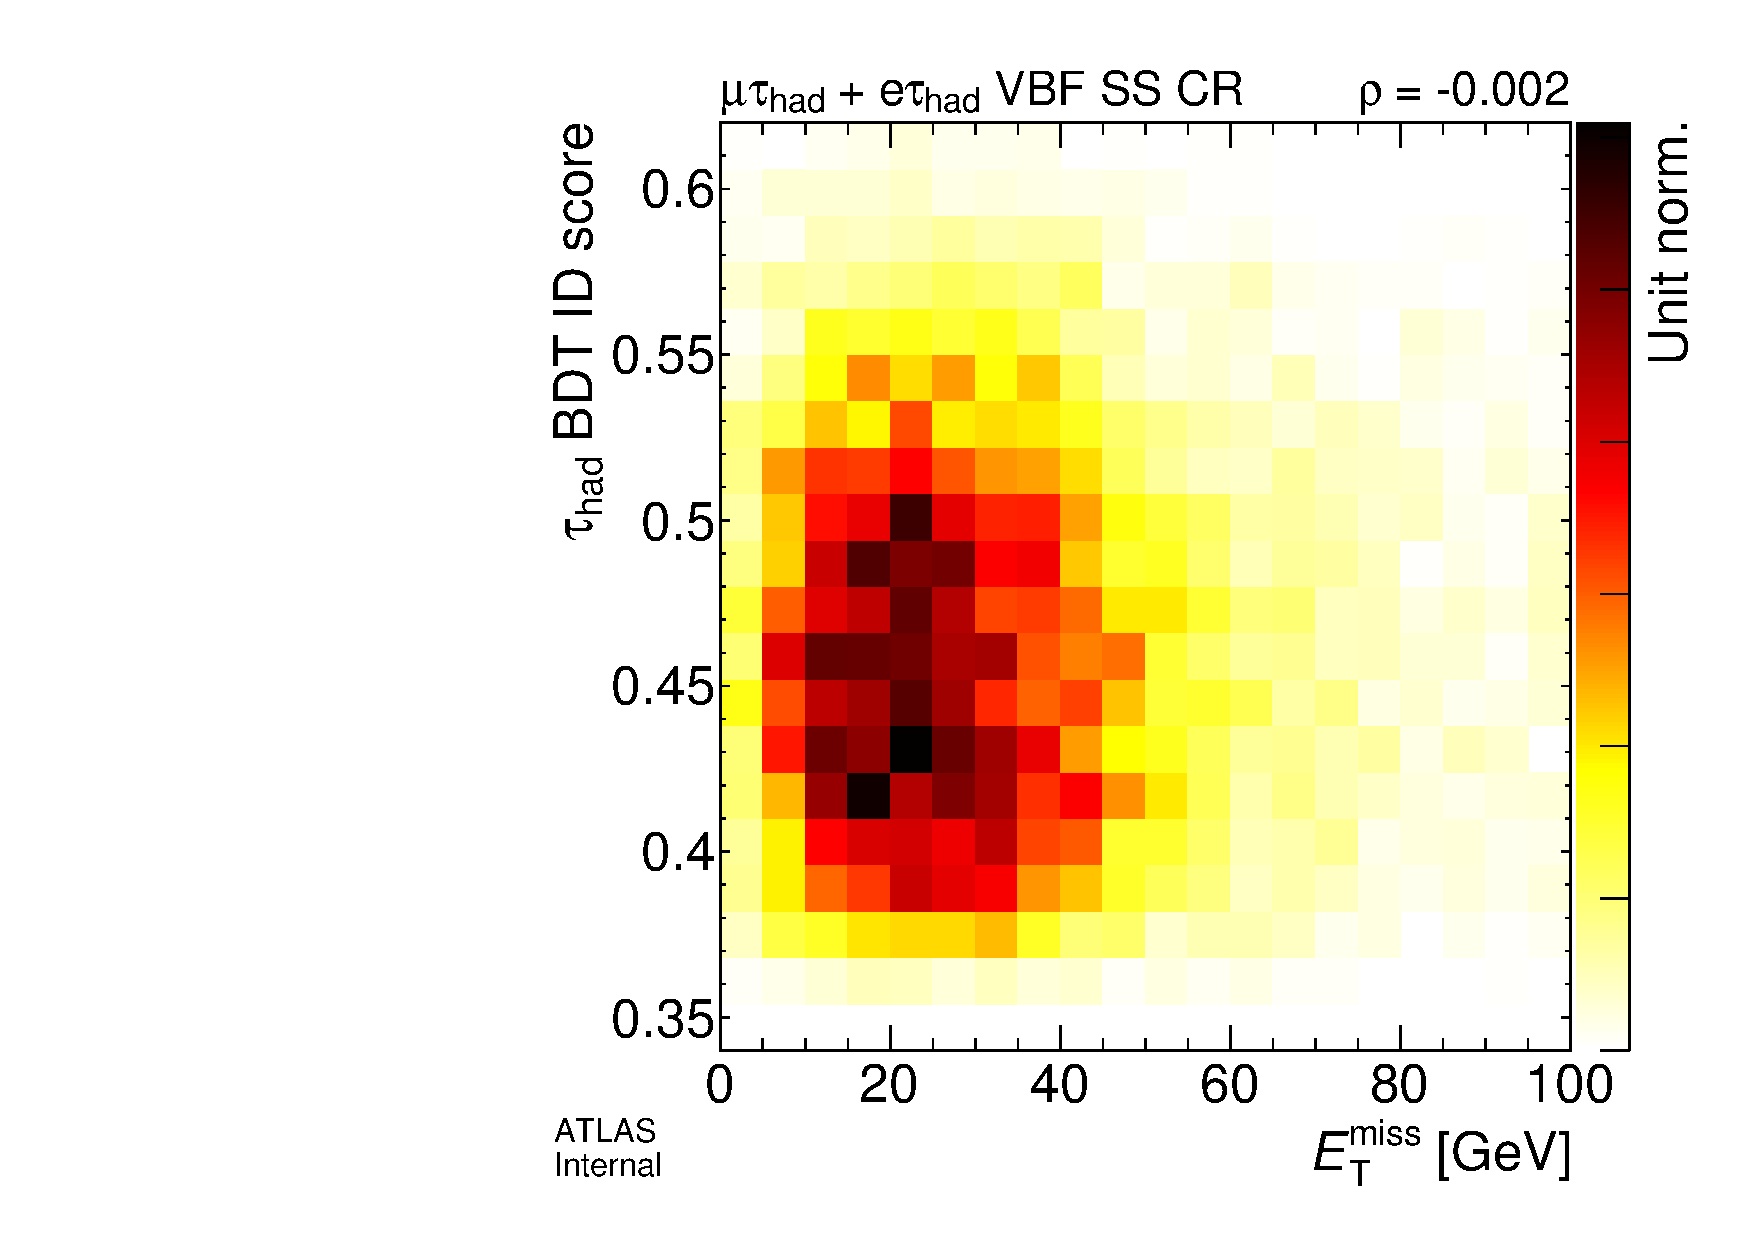
\includegraphics[width=0.32\textwidth]{figures/tauidcorrelations/tauid_vs_metet}
  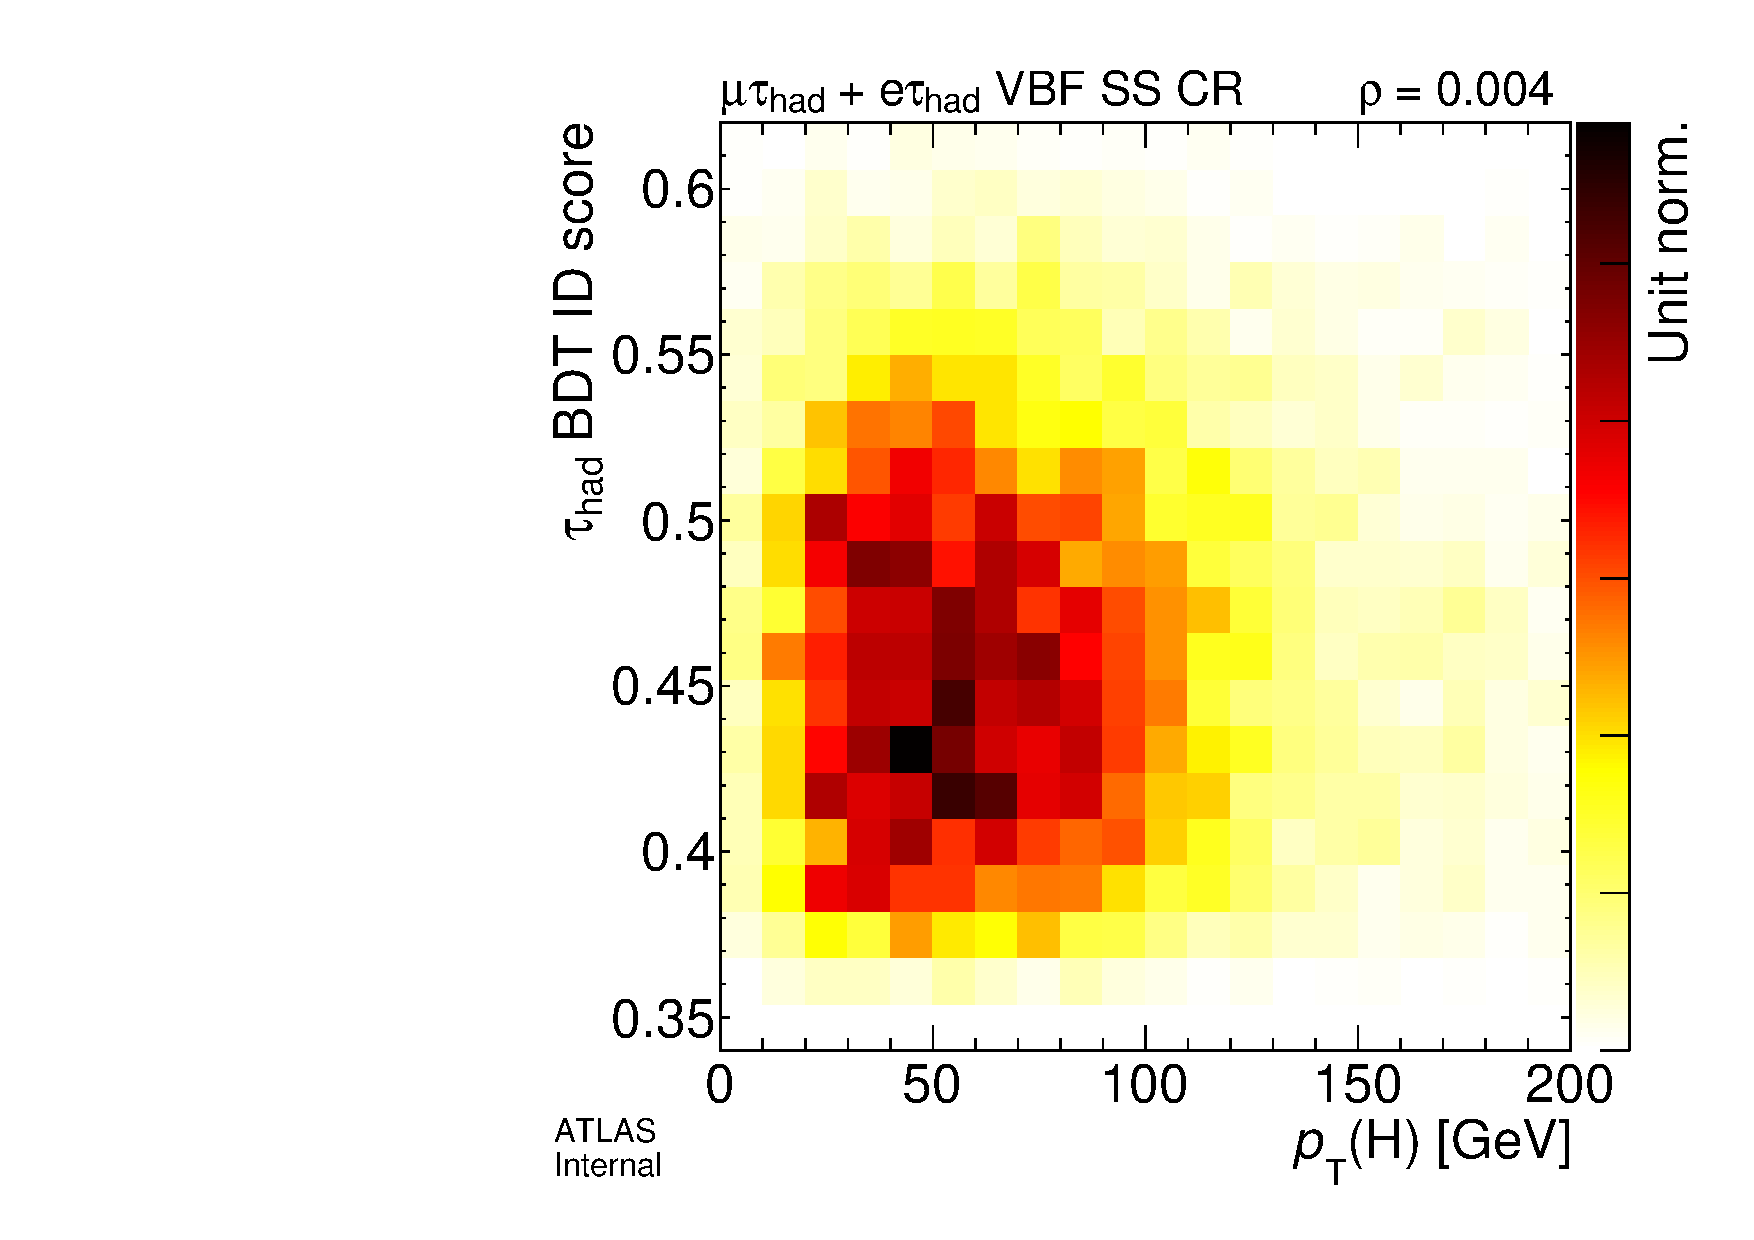
\includegraphics[width=0.32\textwidth]{figures/tauidcorrelations/tauid_vs_Hpt}
  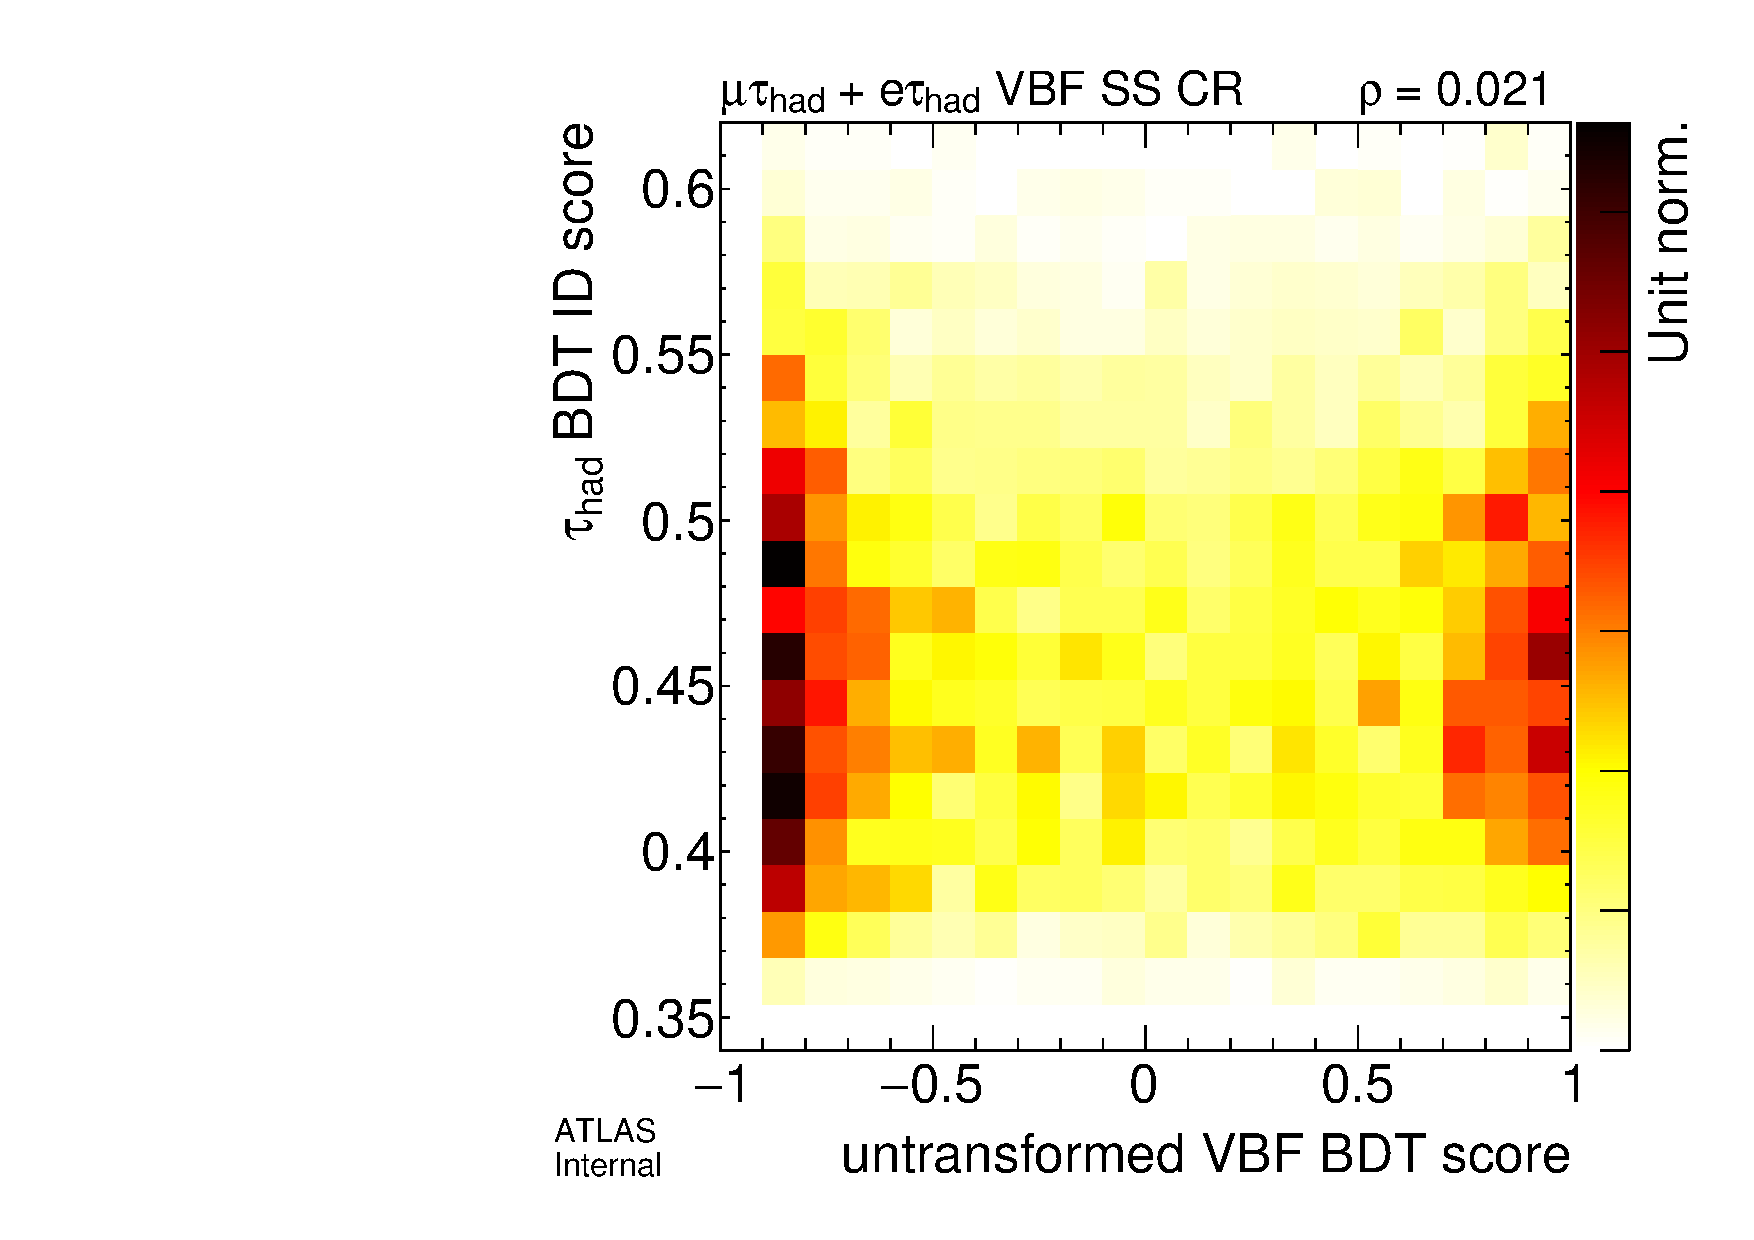
\includegraphics[width=0.32\textwidth]{figures/tauidcorrelations/tauid_vs_bdt}
  \caption{Correlations between the $\tauh$ BDT identification score and event kinematics in data events in the VBF same-sign region which fail $\tauh$ identification but fulfill all other requirements. No strong correlations are observed.}
  \label{fig:backgrounds-tauid-correlations}
\end{figure}

\clearpage

\subsubsection{Implementation}

The $\fakes$ prediction is written as:
%
\begin{equation}
  \begin{split}
    N_{\fakes} &= \left(N_\text{data}^\text{fail ID} - N_{\contam}^\text{fail ID}\right) \times \FF_\text{SR} \\
  \end{split}
  \label{eqn:fakes-prediction}
\end{equation}
%
where the number of predicted $\fakes$ events $N_{\fakes}$ is derived in each bin of any kinematic variable, like $\mjj$. The transfer factor needed to weight data events which fail $\tauh$ identification is called the fakefactor (FF). It is parameterized in the number of tracks associated to the $\tauh$ and $\pt(\tauh)$, and it is derived in a variety of regions rich in different $\fakes$ processes:
%
\begin{equation}
  \begin{split}
    \FF_\text{region} &= \frac{\left(N_\text{data}^\text{pass ID} - N_{\contam}^\text{pass ID}\right)}{\left(N_\text{data}^\text{fail ID} - N_{\contam}^\text{fail ID}\right)} \Bigg\rvert_\text{region} \\
  \end{split}
  \label{eqn:fakes-fakefactor}
\end{equation}
%
where the regions considered here are rich in $\fakes$ from $\Wjets$, QCD, $\Zjets$, or top events, or the same-sign region, which is a blend of $\fakes$ processes. These regions are shown pictorially in \cref{fig:backgrounds-regions}.

\begin{figure}[tp]
  \centering
  \includegraphics[width=0.90\textwidth]{figures/backgrounds/regions-cartoon}
  \caption{Cartoon of the signal, control, and validation regions used which are used in the $\fakes$ estimate.}
  \label{fig:backgrounds-regions}
\end{figure}

To mitigate potential extrapolation costs, $\tauh$ candidates failing identification criteria are required to pass a looser-than-\texttt{loose} requirement. This requirement is optimized to minimize the extrapolation without sacrificing the statistics of the estimate, and a requirement of $\veryloose$ is chosen. For example, if the \texttt{loose} identification criteria requires the $\tauh$ BDT score greater than 0.5, the $\veryloose$ identification criteria requires greater than 0.35. The $\pt(\tauh)$ dependence of this requirement is shown in \cref{fig:backgrounds-workingpoints}.

\begin{figure}[tp]
  \centering
  \includegraphics[width=0.48\textwidth]{figures/backgrounds/jetBDT-1p}
  \includegraphics[width=0.48\textwidth]{figures/backgrounds/jetBDT-3p}
  \caption{Requirements on the $\tauh$ jet discriminant, which are defined to have constant signal efficiency as a function of $\pt(\tauh)$, of various operating points for 1-track $\tauh$ (left) and 3-track $\tauh$ (right).}
  \label{fig:backgrounds-workingpoints}
\end{figure}

The impact of requiring $\veryloose$ can be seen by considering the response of various flavors of $\fakes$ to the tau identification BDT, as shown in $\Wjets$ simulation in \cref{fig:backgrounds-flavors}. This requirement reduces the pileup and gluon content of the anti-identified region and gives it a closer flavor resemblance to the identified region.

\begin{figure}[tp]
  \centering
  \includegraphics[width=0.48\textwidth]{figures/backgrounds/antitau_partonflavor_1p0jSR}
  \includegraphics[width=0.48\textwidth]{figures/backgrounds/antitau_partonflavor_3p0jSR}
  \caption{Predicted flavor composition of $\fakes$ in $\Wjets$ simulation for 1-track $\tauh$ (left) and 3-track $\tauh$ (right).}
  \label{fig:backgrounds-flavors}
\end{figure}

The fakefactors measured in data in the $\Wjets$, QCD, $\Zjets$, and top control regions are shown in \cref{fig:backgrounds-fakefactorsVBFCRs} for 1-track and 3-track $\tauh$ in the VBF category. The measured fakefactors do not show systematic differences between regions given the statistical uncertainty.

\begin{figure}[tp]
  \centering
  \includegraphics[width=0.48\textwidth]{figures/backgrounds/fakefactor_8TeV_vbf_1p_CRs}
  \includegraphics[width=0.48\textwidth]{figures/backgrounds/fakefactor_8TeV_vbf_3p_CRs}
  \caption{Fake factors in the VBF category measured in the various control regions in data for 1-track $\tauh$ (left) and 3-track $\tauh$ (right).}
  \label{fig:backgrounds-fakefactorsVBFCRs}
\end{figure}

\subsubsection{Composition of $\fakes$ in the SR}

A fakefactor for the signal region can be derived from fakefactors measured in the control regions by using simulation to predict the relative contributions of the $\Wjets$, top, and $\Zjets$ processes in the anti-identified region. The remaining difference between data and prediction is then assumed to be from QCD.

The overall relative contributions are shown in \cref{fig:backgrounds-rx-vbf}, and the differential contributions are shown in \cref{fig:backgrounds-rx-vbf-taus,fig:backgrounds-rx-vbf-jets}. No strong dependence on the final VBF BDT discriminator is observed, though dependencies are observed on distributions like $\pt(\text{lepton})$ and $\MET$.

\begin{figure}[tp]
  \centering
  \includegraphics[width=0.90\textwidth]{figures/backgrounds/rx-vbf}
  \caption{A pie chart of the composition of $\fakes$ processes in the anti-identified CR as predicted by simulation and data (left) and the systematic variations on the composition (right).}
  \label{fig:backgrounds-rx-vbf}
\end{figure}

\clearpage

\begin{figure}[tp]
  \centering
  \includegraphics[width=0.32\textwidth]{figures/rx/vbf-mvaSR/tau-pt}
  \includegraphics[width=0.32\textwidth]{figures/rx/vbf-mvaSR/tau-eta}
  \includegraphics[width=0.32\textwidth]{figures/rx/vbf-mvaSR/tau-numTrack}
  % --------------
  \includegraphics[width=0.32\textwidth]{figures/rx/vbf-mvaSR/lep-pt-hi}
  \includegraphics[width=0.32\textwidth]{figures/rx/vbf-mvaSR/lep-eta}
  \includegraphics[width=0.32\textwidth]{figures/rx/vbf-mvaSR/taulep-dR}
  % --------------
  \includegraphics[width=0.32\textwidth]{figures/rx/vbf-mvaSR/met-pt-hi}
  \includegraphics[width=0.32\textwidth]{figures/rx/vbf-mvaSR/mMMC}
  \includegraphics[width=0.32\textwidth]{figures/rx/vbf-mvaSR/mT}
  % --------------
  \includegraphics[width=0.32\textwidth]{figures/rx/vbf-mvaSR/met-phi-centrality}
  \includegraphics[width=0.32\textwidth]{figures/rx/vbf-mvaSR/H-pt-hi}
  \includegraphics[width=0.32\textwidth]{figures/rx/vbf-mvaSR/mvis}
  \caption{The composition of $\fakes$ processes in the anti-identified CR as predicted by simulation and data as a function of event kinematics.}
  \label{fig:backgrounds-rx-vbf-taus}
\end{figure}

\clearpage

\begin{figure}[tp]
  \centering
  \includegraphics[width=0.32\textwidth]{figures/rx/vbf-mvaSR/jet-1-pt}
  \includegraphics[width=0.32\textwidth]{figures/rx/vbf-mvaSR/jet-1-eta}
  \includegraphics[width=0.32\textwidth]{figures/rx/vbf-mvaSR/jets-dphi}
  % --------------
  \includegraphics[width=0.32\textwidth]{figures/rx/vbf-mvaSR/jet-2-pt}
  \includegraphics[width=0.32\textwidth]{figures/rx/vbf-mvaSR/jet-2-eta}
  \includegraphics[width=0.32\textwidth]{figures/rx/vbf-mvaSR/jets-deta}
  % --------------
  \includegraphics[width=0.32\textwidth]{figures/rx/vbf-mvaSR/jets-etaprod}
  \includegraphics[width=0.32\textwidth]{figures/rx/vbf-mvaSR/lep-eta-centrality}
  \includegraphics[width=0.32\textwidth]{figures/rx/vbf-mvaSR/system-pt}
  % --------------
  \includegraphics[width=0.32\textwidth]{figures/rx/vbf-mvaSR/n-jets30}
  \includegraphics[width=0.32\textwidth]{figures/rx/vbf-mvaSR/dijet-m-veryhigh}
  \includegraphics[width=0.32\textwidth]{figures/rx/vbf-mvaSR/BDTEve-VBF}
  \caption{The composition of $\fakes$ processes in the anti-identified CR as predicted by simulation and data as a function of event kinematics.}
  \label{fig:backgrounds-rx-vbf-jets}
\end{figure}

The signal region fakefactors are then derived as a linear combination of control region fakefactors weighted by the expected contributions. The systematic uncertainties on these contributions is shown in \cref{fig:backgrounds-rx-vbf}. A conservative approach is taken due to the mistrust of simulated $\fakes$, and the contribution from $\Wjets$ is allowed to double or halve as the two variations.

The signal region fakefactors are shown in \cref{fig:backgrounds-fakefactorsVBFmix}. These are also referred to as mixed fakefactors. Since the control region fakefactors do not have significant differences between them, the dominant uncertainty on the signal region fakefactors is typically statistical.

\begin{figure}[tp]
  \centering
  \includegraphics[width=0.48\textwidth]{figures/backgrounds/fakefactor_8TeV_vbf_1p_mix}
  \includegraphics[width=0.48\textwidth]{figures/backgrounds/fakefactor_8TeV_vbf_3p_mix}
  \caption{Fake factors in the VBF category mixed from the various control regions in data for 1-track $\tauh$ (left) and 3-track $\tauh$ (right). Statistical and systematic uncertainties are shown.}
  \label{fig:backgrounds-fakefactorsVBFmix}
\end{figure}

\clearpage

\subsection{Validation}

The fakefactor method is validated by checking predictions of event-level kinematics, especially the BDT discriminant, in the control and validation regions. It is additionally validated by following the same fakefactor procedure in $\Wjets$, top, and $\Zjets$ simulated events in the signal region, where dedicated $\FF_\text{SR}^\text{MC}$ are derived.

Data and prediction in the same-sign validation region are shown in \cref{fig:backgrounds-SSXCR-taus,fig:backgrounds-SSXCR-jets}. Data and prediction in the various control regions are further shown in \cref{apx:control-regions}. Predictions with simulation are shown in \cref{fig:backgrounds-MCXSR-taus,fig:backgrounds-MCXSR-jets}. In all plots, good agreement is observed and no systematic biases are uncovered.

\clearpage

\begin{figure}[tp]
  \centering
  \includegraphics[width=0.32\textwidth]{figures/analysis/vbf-SSXCR/tau-pt}
  \includegraphics[width=0.32\textwidth]{figures/analysis/vbf-SSXCR/tau-eta}
  \includegraphics[width=0.32\textwidth]{figures/analysis/vbf-SSXCR/tau-numTrack} \\
  \includegraphics[width=0.32\textwidth]{figures/analysis/vbf-SSXCR/lep-pt-hi}
  \includegraphics[width=0.32\textwidth]{figures/analysis/vbf-SSXCR/lep-eta}
  \includegraphics[width=0.32\textwidth]{figures/analysis/vbf-SSXCR/taulep-dR} \\
  \includegraphics[width=0.32\textwidth]{figures/analysis/vbf-SSXCR/met-pt-hi}
  \includegraphics[width=0.32\textwidth]{figures/analysis/vbf-SSXCR/mMMC}
  \includegraphics[width=0.32\textwidth]{figures/analysis/vbf-SSXCR/mT} \\
  \includegraphics[width=0.32\textwidth]{figures/analysis/vbf-SSXCR/met-phi-centrality}
  \includegraphics[width=0.32\textwidth]{figures/analysis/vbf-SSXCR/H-pt-hi}
  \includegraphics[width=0.32\textwidth]{figures/analysis/vbf-SSXCR/mvis} \\
  \caption{Comparison of data and $\fakes$ prediction in the same-sign validation region for various event kinematics. The purity of $\fakes$ is $\approx\! 97\%$. Only statistical uncertainties are shown, and no sign of systematic bias is observed.}
  \label{fig:backgrounds-SSXCR-taus}
\end{figure}

\clearpage

\begin{figure}[tp]
  \centering
  \includegraphics[width=0.32\textwidth]{figures/analysis/vbf-SSXCR/jet-1-pt}
  \includegraphics[width=0.32\textwidth]{figures/analysis/vbf-SSXCR/jet-1-eta}
  \includegraphics[width=0.32\textwidth]{figures/analysis/vbf-SSXCR/jets-dphi} \\
  \includegraphics[width=0.32\textwidth]{figures/analysis/vbf-SSXCR/jet-2-pt}
  \includegraphics[width=0.32\textwidth]{figures/analysis/vbf-SSXCR/jet-2-eta}
  \includegraphics[width=0.32\textwidth]{figures/analysis/vbf-SSXCR/jets-deta} \\
  \includegraphics[width=0.32\textwidth]{figures/analysis/vbf-SSXCR/jets-etaprod} 
  \includegraphics[width=0.32\textwidth]{figures/analysis/vbf-SSXCR/lep-eta-centrality}
  \includegraphics[width=0.32\textwidth]{figures/analysis/vbf-SSXCR/system-pt} \\
  \includegraphics[width=0.32\textwidth]{figures/analysis/vbf-SSXCR/n-jets30}
  \includegraphics[width=0.32\textwidth]{figures/analysis/vbf-SSXCR/dijet-m-veryhigh}
  \includegraphics[width=0.32\textwidth]{figures/analysis/vbf-SSXCR/BDTEve-VBF} \\
  \caption{Comparison of data and $\fakes$ prediction in the same-sign validation region for various event kinematics. The purity of $\fakes$ is $\approx\! 97\%$. Only statistical uncertainties are shown, and no sign of systematic bias is observed.}
  \label{fig:backgrounds-SSXCR-jets}
\end{figure}

\clearpage

\begin{figure}[tp]
  \centering
  \includegraphics[width=0.32\textwidth]{figures/analysis/vbf-MCXSR/tau-pt}
  \includegraphics[width=0.32\textwidth]{figures/analysis/vbf-MCXSR/tau-eta}
  \includegraphics[width=0.32\textwidth]{figures/analysis/vbf-MCXSR/tau-numTrack} \\
  \includegraphics[width=0.32\textwidth]{figures/analysis/vbf-MCXSR/lep-pt-hi}
  \includegraphics[width=0.32\textwidth]{figures/analysis/vbf-MCXSR/lep-eta}
  \includegraphics[width=0.32\textwidth]{figures/analysis/vbf-MCXSR/taulep-dR} \\
  \includegraphics[width=0.32\textwidth]{figures/analysis/vbf-MCXSR/met-pt-hi}
  \includegraphics[width=0.32\textwidth]{figures/analysis/vbf-MCXSR/mMMC}
  \includegraphics[width=0.32\textwidth]{figures/analysis/vbf-MCXSR/mT} \\
  \includegraphics[width=0.32\textwidth]{figures/analysis/vbf-MCXSR/met-phi-centrality}
  \includegraphics[width=0.32\textwidth]{figures/analysis/vbf-MCXSR/H-pt-hi}
  \includegraphics[width=0.32\textwidth]{figures/analysis/vbf-MCXSR/mvis} \\
  \caption{Comparison of the prediction of identified taus and the $\fakes$ prediction, both in simulation, in the signal region for various event kinematics. Only statistical uncertainties are shown, and no sign of systematic bias is observed.}
  \label{fig:backgrounds-MCXSR-taus}
\end{figure}

\clearpage

\begin{figure}[tp]
  \centering
  \includegraphics[width=0.32\textwidth]{figures/analysis/vbf-MCXSR/jet-1-pt}
  \includegraphics[width=0.32\textwidth]{figures/analysis/vbf-MCXSR/jet-1-eta}
  \includegraphics[width=0.32\textwidth]{figures/analysis/vbf-MCXSR/jets-dphi} \\
  \includegraphics[width=0.32\textwidth]{figures/analysis/vbf-MCXSR/jet-2-pt}
  \includegraphics[width=0.32\textwidth]{figures/analysis/vbf-MCXSR/jet-2-eta}
  \includegraphics[width=0.32\textwidth]{figures/analysis/vbf-MCXSR/jets-deta} \\
  \includegraphics[width=0.32\textwidth]{figures/analysis/vbf-MCXSR/jets-etaprod} 
  \includegraphics[width=0.32\textwidth]{figures/analysis/vbf-MCXSR/lep-eta-centrality}
  \includegraphics[width=0.32\textwidth]{figures/analysis/vbf-MCXSR/system-pt} \\
  \includegraphics[width=0.32\textwidth]{figures/analysis/vbf-MCXSR/n-jets30}
  \includegraphics[width=0.32\textwidth]{figures/analysis/vbf-MCXSR/dijet-m-high}
  \includegraphics[width=0.32\textwidth]{figures/analysis/vbf-MCXSR/BDTEve-VBF} \\
  \caption{Comparison of the prediction of identified taus and the $\fakes$ prediction, both in simulation, in the signal region for various event kinematics. Only statistical uncertainties are shown, and no sign of systematic bias is observed.}
  \label{fig:backgrounds-MCXSR-jets}
\end{figure}

\clearpage

\subsection{Uncertainties}

Multiple sources of uncertainties to the fake factor method are considered. First, the statistical uncertainty on the fake factors measured in control regions is propagated to the uncertainty on the signal region fakefactor. Second, the uncertainty on the relative contributions of the different $\fakes$ processes are varied and propagated to the signal region fakefactor calculation. Third, the fidelity of using control region fakefactors in the signal region is tested by comparing fakefactors measured in simulation in control regions versus the signal region. No significant difference is found, and the uncertainty is ignored. Fourth, the closure of the method is tested with predictions in the same sign validation region and in the signal region in simulation. No signs of systematic bias in the BDT score prediction are found, and the closure uncertainties are ignored.

The pre-fit impact of these uncertainties on the $\fakes$ prediction is shown in each bin of the VBF discriminator in \cref{fig:backgrounds-uncertainties-fakes}. The largest uncertainty at high VBF BDT score is the 15\% statistical uncertainty on the prediction. This could be ameliorated by relaxing the $\veryloose$ requirement on anti-identified $\tauh$, though this would risk introducing systematic bias of increasing the extrapolation. The largest systematic uncertainty is on the relative contribution of $\fakes$ processes, and this only propagates to a 3\% uncertainty on the prediction.

\begin{figure}[tp]
  \includegraphics[width=0.90\textwidth]{figures/uncertainties/uncertainties_lephad_paper14_8TeV_fakes_VBF}
  \caption{The pre-fit fractional uncertainty on the $\fakes$ prediction in each bin of the VBF category. $\text{R}_\text{X}$ refers to the uncertainty on the relative contribution of $\fakes$ processes.}
  \label{fig:backgrounds-uncertainties-fakes}
\end{figure}

\clearpage

\section{top, $\Zll$, diboson}
\label{sec:backgrounds-others}

\subsection{top}

Top events with a true $\tauh$ or $\lfake$ are estimated with simulation and object-level corrections prescribed by the $\tauh$ performance group. These include $t\overline{t}$ and single top processes. The normalization is constrained using a top-enriched control region, but detailed corrections to the simulation are not sought because the background is sub-dominant. These top processes only comprise 5\% of the background prediction in the VBF category and in the most sensitive bin of the VBF BDT discriminator.

\subsection{$\Zll$ ($\lfake$), diboson}

$\Zll$ events where a lepton is mis-identified as a $\tauh$ and diboson events ($WW$, $WZ$, $ZZ$) are estimated with simulation and object-level corrections prescribed by the $\tauh$ performance group. Control regions for these processes are not sought because the processes are too small to find meaningful regions for comparing data with simulation. Detailed corrections to the simulation are also not sought because each processes comprises less than 5\% of the background prediction in the VBF category and in the most sensitive bin of the VBF BDT discriminator.

The $\tauh$ electron discriminator reduces the $\Zee$ background from problematic to negligible, as shown in \cref{fig:backgrounds-zll}. Without the electron discriminator, the VBF $\Zee$ background would be difficult to distinguish from VBF $\Htautau$ and potentially of comparable magnitude.

\begin{figure}[tp]
  \includegraphics[width=0.48\textwidth]{figures/backgrounds/mvis-with-eveto.pdf}
  \includegraphics[width=0.48\textwidth]{figures/backgrounds/mvis-without-eveto.pdf}
  \caption{Data and prediction for the nominal VBF category (left) and without the $\tauh$ electron discriminator (right).}
  \label{fig:backgrounds-zll}
\end{figure}

\section{$\Htautau$}
\label{sec:backgrounds-htautau}

\subsection{Samples}

The signal $\Htautau$ processes are simulated with \textsc{Powheg+Pythia} (ggFH, VBFH) and \textsc{Pythia} (WH, ZH, ttH)~\cite{HIGG-2013-32}, though the VH and ttH processes are generally negligible in the signal regions considered. The overall normalisation of the  ggF process is taken from a calculation at next-to-next-to-leading-order (NNLO) in QCD, including soft-gluon resummation up to next-to-next-to-leading logarithm terms (NNLL). Next-to-leading order (NLO) EW corrections are also included.  Production by VBF is normalised to a cross section calculated with full NLO QCD and EW corrections with an approximate NNLO QCD correction applied.

Additional corrections to the shape of the generated $\pt$ distribution of Higgs bosons produced via ggF are applied to match the distribution from a calculation at NNLO including the NNLL corrections provided by the \textsc{HRes2.1} program~\cite{HIGG-2013-32}. In this calculation, the effects of finite masses of the top and bottom quarks are included and dynamical renormalisation and factorisation scales, $\mu_\mathrm{R},\mu_\mathrm{F} = \sqrt{m_{H}^2 + \pt^2}$, are used.  A reweighting is performed separately for events with no more than one jet at particle level and for events with two or more jets. In the latter case, the Higgs boson $\pt$ spectrum is reweighted to match the \textsc{MinLo HJJ} predictions. The reweighting is derived such that the inclusive Higgs boson $\pt$ spectrum and the $\pt$ spectrum of events with at least two jets match the \textsc{HRes2.1} and \textsc{MinLo HJJ} predictions respectively, and that the jet multiplicities are in agreement with (N)NLO calculations from \textsc{JetVHeto}. A similar $\pt$-dependent weighting is derived for NLO EW corrections of the VBFH production using \textsc{Hawk}, though the corrections are small in the $\pt$ ranges considered here~\cite{HIGG-2013-32}.

\subsection{Uncertainties}

\begin{figure}[tp]
  \includegraphics[width=0.85\textwidth]{figures/uncertainties/uncertainties_lephad_paper14_8TeV_VBFH125_JES_VBF}
  \includegraphics[width=0.85\textwidth]{figures/uncertainties/uncertainties_lephad_paper14_8TeV_VBFH125_other_VBF}
  \caption{The pre-fit fractional uncertainty on the VBF $\Htautaulh$ prediction in each bin of the VBF category for uncertainties pertaining to the jet energy scale (top) and $\tauh$ performance, theory, and the luminosity (bottom).}
  \label{fig:backgrounds-uncertainties-vbf}
\end{figure}

